\documentclass[12pt,a4paper]{report}

\setcounter{tocdepth}{3} % Include subsubsection in TOC
\setcounter{secnumdepth}{3} %number subsubsections in TOC
%\usepackage[utf8]{inputenc}
%\usepackage[T1]{fontenc}
\usepackage{graphicx}
\usepackage{geometry}
\usepackage{multicol}
\usepackage{array}
\usepackage{fancyhdr}

\usepackage{lipsum}
\usepackage{appendix}

% Load fontspec and polyglossia before biblatex
\usepackage{fontspec}
\usepackage{bidi}
\usepackage{polyglossia}
\setmainlanguage{english}
\setotherlanguages{french}
\newfontfamily\frenchfont{Times New Roman}
\newfontfamily\arabicfont[Script=Arabic]{Amiri}


% Load biblatex after polyglossia
\usepackage[backend=biber,style=ieee]{biblatex}
\addbibresource{references.bib}

\renewcommand{\arraystretch}{0.85} % Tighter vertical spacing
\usepackage{setspace}
\usepackage[justification=centering]{caption}
\usepackage{indentfirst}

% Set headheight before loading fancyhdr to avoid warnings
\setlength{\headheight}{27.42pt}
\usepackage{fancyhdr}
\usepackage[hidelinks]{hyperref}
\usepackage[acronym]{glossaries}
\makeglossaries
\usepackage{float}
\usepackage{adjustbox}
\usepackage{listings}
\usepackage{xcolor}
\usepackage{tikz}

\usetikzlibrary{arrows.meta, positioning, shapes.misc, fit, backgrounds, calc}
\usetikzlibrary{shapes.geometric}
\tikzstyle{startstop} = [rectangle, rounded corners, minimum width=3cm, minimum height=1cm,text centered, draw=black, fill=red!30]
\tikzstyle{process} = [rectangle, minimum width=3.5cm, minimum height=1cm, text centered, draw=black, fill=blue!20]
\tikzstyle{decision} = [diamond, aspect=2, text centered, draw=black, fill=green!20]
\tikzstyle{arrow} = [thick,->,>=stealth]
\tikzstyle{startstop} = [rectangle, rounded corners, minimum width=3.2cm, minimum height=0.9cm, text centered, draw=black]
\tikzstyle{process}   = [rectangle, minimum width=3.6cm, minimum height=0.9cm, text centered, draw=black]
\tikzstyle{decision}  = [diamond, aspect=2, text centered, draw=black, inner sep=1pt]
\tikzstyle{arrow}     = [thick,->,>=stealth]
\lstdefinelanguage{json}{
    basicstyle=\ttfamily,
    showstringspaces=false,
    morestring=[b]",
    morecomment=[l]{//},
    morekeywords={true,false,null},
    keywordstyle=\color{blue},
    stringstyle=\color{black},
    commentstyle=\color{gray}
}

% --- Define acronyms ---
\newacronym{evtol}{eVTOL}{electric Vertical Take-Off and Landing}
\newacronym{wis}{WIS}{Weather Information Service}
\newacronym{uas}{UAS}{Unmanned Aerial Systems}
\newacronym{easa}{EASA}{European Union Aviation Safety Agency}
\newacronym{metar}{METAR}{Meteorological Aerodrome Report}
\newacronym{api}{API}{Application Programming Interface}
\newacronym{rest}{REST}{Representational State Transfer}
\newacronym{oauth2}{OAuth2}{Open Authorization 2.0}
\newacronym{aam}{AAM}{Advanced Air Mobility}
\newacronym{dxb}{DXB}{Dubai International Airport}
\newacronym{rta}{RTA}{Roads and Transport Authority}
\newacronym{vfr}{VFR}{Visual Flight Rules}
\newacronym{uav}{UAV}{Unmanned Aerial Vehicle}
\newacronym{aws}{AWS}{Amazon Web Services}
\newacronym{dxv}{DXV}{Dubai International Vertiport}
\newacronym{revpi}{RevPi}{Revolution Pi}
\newacronym{uam}{UAM}{Urban Air Mobility}
\newacronym{notams}{NOTAMs}{Notice to Air Missions}
\newacronym{bvlos}{BVLOS}{Beyond Visual Line of Sight}
\newacronym{ceo}{CEO}{Chief Executive Officer}
\newacronym{cto}{CTO}{Chief Technology Officer}
\newacronym{coo}{COO}{Chief Operating Officer}
\newacronym{venv}{venv}{Virtual Environment}
\newacronym{din}{DIN}{Deutsches Institut für Normung}
\newacronym{ascii}{ASCII}{American Standard Code for Information Interchange}
\newacronym{crc}{CRC}{Cyclic Redundancy Check}
\newacronym{ssh}{SSH}{Secure Shell}
\newacronym{ip}{IP}{Internet Protocol}
\newacronym{rtu}{RTU}{Remote Terminal Unit}
\newacronym{ttl}{TTL}{Time-to-Live}
\newacronym{vcs}{VCS}{Version Control System}
\newacronym{mor}{MOR}{Meteorological Optical Range}
\newacronym{ip66}{IP66}{Ingress Protection rating 66}
\newacronym{emc}{EMC}{Electromagnetic Compatibility}
\newacronym{en61326}{EN61326-1}{European standard for EMC requirements}
\newacronym{pwd12}{PWD12}{Present Weather Detector 12}
\newacronym{nws}{NWS}{National Weather Service}
\newacronym{wmo}{WMO}{World Meteorological Organization}
\newacronym{rs485}{RS-485}{Recommended Standard 485}
\newacronym{hvac}{HVAC}{Heating, Vnetilation, and Air Conditioning}
\newacronym{rs232}{RS-232}{Recommended Standard 232}
\newacronym{emi}{EMI}{Electromagnetic Interference}
\newacronym{usb}{USB}{Universal Serial Bus}
\newacronym{cr}{CR}{Carriage Return}
\newacronym{synop}{SYNOP}{Surface Synoptic Observation}
\newacronym{json}{JSON}{JavaScript Object Notation}
\newacronym{utc}{UTC}{Coordinated Universal Time}
\newacronym{dns}{DNS}{Domain Name System}
\newacronym{acid}{ACID}{Atomicity, Consistency, Isolation, and Durability}
\newacronym{uv}{UV}{Ultra-Violet}
\newacronym{fifo}{FIFO}{First In First Out}
\newacronym{cli}{CLI}{Command Line Interface}
\newacronym{cicd}{CI/CD}{Continuous Integration and Continuous Delivery/Deployment}
\newacronym{iot}{IoT}{Internet of Things}


\geometry{left=2cm, right=2cm, top=2cm, bottom=2cm}

\begin{document}
\onehalfspacing


\begin{titlepage}
    \begin{center}
        \begin{tabular}{ m{2.5cm} m{10cm} m{2.5cm} }
            
\includegraphics[width=2.5cm]{images/insat.jpg} &
            \centering
            \begin{minipage}[c]{\linewidth}
                \centering
                {\small \textbf{REPUBLIC OF TUNISIA}}\\[0.15cm]
                {\small Ministry of Higher Education and Scientific Research}\\[0.15cm]
                {\small University of Carthage}\\[0.15cm]
                {\small National Institute of Applied Sciences and Technology}
            \end{minipage}
            &
            
\includegraphics[width=2.5cm]{images/unicar.png} \\
        \end{tabular}
    \end{center}
   
    \vspace{0.5cm}
\noindent\rule{\textwidth}{0.4pt}


\begin{center}
    \LARGE \textbf{Graduation Project}\\[0.4cm]
    \normalsize to obtain the\\[0.4cm]
    \LARGE \textbf{National Engineering Diploma}\\[0.4cm]
    \normalsize in Applied Sciences and Technology\\[0.4cm]
    \normalsize \textbf{Specialty: Instrumentation and Industrial Maintenance}\\[0.5cm]
    \rule{10cm}{0.5pt}\\[0.4cm]
    \Large \textbf{Development of an IOT-based Weather Sensor System for Drone Operations}\\
    \rule{10cm}{0.5pt}\\[0.4cm]
    \normalsize Prepared by\\[0.4cm]
    \large \textbf{Mahdi MAJJEDI}\\[0.4cm]
    \normalsize Hosted by Unisphere GmbH\\[0.4cm]
    
\includegraphics[width=6cm]{images/unisphere.png}\\[0.4cm]
    \normalsize Defended on 25/09/2025 in front of a jury composed of:\\[0.4cm]
    \begin{tabular}{@{} r l @{}}
        \large \textbf{Mr. Atef BOULILA} & \large President of the jury \\[0.3cm]
        \large \textbf{Mr. Saber TLILI} & \large Reviewer \\[0.3cm]
        \large \textbf{Ms. Imen JAAFAR}       & \large Supervisor at INSAT \\[0.3cm]
        \large \textbf{Mr. Michael ANGER}     & \large Supervisor at the Company \\[1cm]
    \end{tabular}
    
    {\normalsize \textbf{School year: 2024/2025}}\\
\end{center}



\end{titlepage}

\newpage

\begin{titlepage}
    \begin{center}
        \begin{tabular}{ m{2.5cm} m{10cm} m{2.5cm} }
            
\includegraphics[width=2.5cm]{images/insat.jpg} &
            \centering
            \begin{minipage}[c]{\linewidth}
                \centering
                {\small \textbf{REPUBLIC OF TUNISIA}}\\[0.15cm]
                {\small Ministry of Higher Education and Scientific Research}\\[0.15cm]
                {\small University of Carthage}\\[0.15cm]
                {\small National Institute of Applied Sciences and Technology}
            \end{minipage}
            &
            
\includegraphics[width=2.5cm]{images/unicar.png} \\
        \end{tabular}
    \end{center}
   
   
\noindent\rule{\textwidth}{0.4pt}


\begin{center}
    \LARGE \textbf{Graduation Project}\\[0.4cm]
    \normalsize to obtain the\\[0.4cm]
    \LARGE \textbf{National Engineering Diploma}\\[0.4cm]
    \normalsize in Applied Sciences and Technology\\[0.4cm]
    \normalsize \textbf{Specialty: Instrumentation and Industrial Maintenance}\\
    \rule{10cm}{0.5pt}\\
    \Large \textbf{Development of an IOT-based Weather Sensor System for Drone Operations}\\
    \rule{10cm}{0.5pt}\\
    \normalsize Prepared by\\[0.4cm]
    \large \textbf{Mahdi MAJJEDI}\\[0.4cm]
    \normalsize Hosted by Unisphere GmbH\\[0.4cm]
    
\includegraphics[width=6cm]{images/unisphere.png}\\[0.4cm]
    \begin{tabular}{|p{7cm}|p{7cm}|}
        \hline\\
        {\centering Supervisor at the Company \par} & {\centering Supervisor at INSAT \par}\\
        {\centering Mr. Michael ANGER \par} & {\centering Ms. Imen JAAFAR \par}\\
        \hline
        \rule{0pt}{2.5cm} & \rule{0pt}{2.5cm}\\
        Date:  & Date: \\
        \hline
    \end{tabular}

\vspace{0.5cm}

    
    {\normalsize \textbf{School year: 2024/2025}}\\
\end{center}



\end{titlepage}

% Use Roman numbering for front matter (or no numbering)
\pagenumbering{roman}
\pagestyle{plain} % or empty, or fancy if you customize headers

% --- Dedication (not in TOC) ---
\cleardoublepage
\chapter*{Dedication}
\thispagestyle{empty}
\vspace*{2cm}

\begin{center}
\itshape   % Italic for elegance
\setlength{\parskip}{1.2em} % space between paragraphs
\setlength{\parindent}{0pt} % no indentation

To my beloved family—my mother, father, and sister—whose love, encouragement, and unwavering belief in me have been the foundation of my journey. Your constant support gave me the strength to persevere through challenges and the motivation to keep striving for more.

To my extended family, whose kindness and support in many different ways have helped me reach this milestone and made the path smoother along the way.

To my friends, who stood by me with patience, laughter, and understanding, reminding me that even during the busiest and most difficult times, life is brighter when shared.

This work is dedicated to all of you, with gratitude for your emotional support, and with the hope that it reflects the values of learning, growth, and persistence that you have helped instill in me.
\end{center}

\vspace{3em}

\begin{flushright}
\textit{Mahdi Majjedi}
\end{flushright}


% --- Acknowledgements (not in TOC) ---
\cleardoublepage
\chapter*{Acknowledgements}
\thispagestyle{empty}
\vspace*{2cm}
\begin{center}
\itshape   % Italic for elegance
\setlength{\parskip}{1.2em} % space between paragraphs
\setlength{\parindent}{0pt} % no indentation

First and foremost, I would like to express my sincere gratitude to my professor, \textbf{Imen JAAFAR}, for her invaluable guidance, encouragement, and continuous support throughout this thesis project. Her expertise and thoughtful advice were essential in shaping both the technical and academic aspects of this work.

I would also like to thank the members of the \textbf{jury}, who dedicated their time and effort to carefully read this report and evaluate my work. Their contribution ensures that this project is assessed with fairness and rigor, and I deeply appreciate their commitment.

I am profoundly grateful to \textbf{Michael ANGER}, CTO of Unisphere GmbH, for giving me the opportunity to carry out my internship within the company. His trust allowed me to explore a challenging and meaningful project in a stimulating professional environment.

My heartfelt thanks go to \textbf{Michael SCHEER}, software developer at Unisphere, with whom I had the privilege of working closely. His supervision, availability, and constructive feedback were invaluable throughout this journey, and I benefited greatly from his expertise and mentorship.

Finally, I wish to express my appreciation to the entire \textbf{Unisphere team}. Their collaborative spirit, welcoming atmosphere, and unique company culture made this internship not only professionally enriching but also personally memorable.  
\end{center}


% --- Abstract (not in TOC) ---
\cleardoublepage
\chapter*{Abstract}
\thispagestyle{empty}

This thesis presents the integration of the Vaisala \gls{pwd12} visibility sensor into an existing weather station system initially built around a Vaisala WXT536 sensor. The system is deployed on a Revolution Pi industrial controller and serves the needs of Unisphere GmbH, where high-quality, real-time meteorological data is required to support safe and efficient flight monitoring through the NOVA platform.

The work addresses both hardware and software challenges. On the hardware side, the \gls{pwd12} was connected using a dedicated \gls{rs485} interface to ensure compatibility with its baud rate and communication protocol. The wiring design prioritized simplicity and robustness, while maintaining independence between sensors to avoid interference.  

On the software side, the integration followed a modular Python-based approach. Each sensor was assigned its own reader and parser modules, running concurrently under a systemd-managed service. Data acquisition, validation, and parsing pipelines were implemented to produce structured \gls{json} payloads compatible with the existing cloud infrastructure. Particular attention was given to error handling and resilience, including checksum verification and code modularity for future extensibility.  

One of the key contributions of this work is the implementation of local offline buffering through an embedded SQLite database. This ensures data persistence and reliable synchronization with the \acrshort{aws} AppSync GraphQL \gls{api} even during connectivity interruptions. Retry logic and recovery workflows were designed to preserve data integrity and maintain chronological ordering of records during cloud uploads.  

The results demonstrate a resilient and extensible system capable of supporting additional sensors with minimal reconfiguration. The integration of the \gls{pwd12} significantly expands the scope of collected environmental data, particularly by enabling visibility and present weather measurements. This work not only enhances the operational value of the weather station for Unisphere but also provides a modular blueprint for future sensor integrations in similar embedded cloud-connected environments.  


% --- Table of Contents ---
\cleardoublepage
\tableofcontents

% --- List of Figures ---
\cleardoublepage
\listoffigures

% --- List of Tables ---
\cleardoublepage
\listoftables

\cleardoublepage
\lstlistoflistings
% --- List of Acronyms ---



\printacronyms



% --- MAIN MATTER ---

\cleardoublepage
\pagenumbering{arabic} % restart page numbering in Arabic numerals
\setcounter{page}{1}   % start at page 1
\pagestyle{fancy}      % set page style for main chapters
\fancyhead{} % clear all header fields
\fancyhead[L]{\MakeUppercase{\leftmark}} % show chapter name uppercase on left

% Redefine \chaptermark to show only chapter name (no section)
\renewcommand{\chaptermark}[1]{%
\markboth{CHAPTER \thechapter. #1}{}%
}

\chapter*{Introduction}
\addcontentsline{toc}{chapter}{Introduction}

Weather has always been one of the most decisive factors in aviation. 
According to the U.S. Federal Aviation Administration, nearly 26\% of flight delays are directly caused by adverse weather conditions. 
For traditional air traffic, this can mean rerouted flights, extended delays, or cancellations. 
With the rapid development of urban air mobility concepts such as air taxis and drone operations, the challenge becomes even greater: 
these aircraft will fly at lower altitudes, more frequently, and within densely populated environments where local weather phenomena such as fog or sudden precipitation can have an immediate impact on safety.  

Unisphere GmbH is a company that develops digital solutions for flight operations and U-Space services. 
One of its focus areas is providing reliable and localized weather information to support decision-making for manned and unmanned aviation. 
This is achieved through \acrshort{iot}-based weather monitoring solutions, where sensors, edge devices, and cloud platforms are combined to deliver real-time insights for operators.  
Nevertheless, ensuring reliable data flow in field deployments remains a challenge. 
Weather stations must capture all relevant parameters, operate autonomously in harsh environments, and continue functioning even when network connectivity is temporarily unavailable.  

In this context, the present work addresses the problem of extending and reinforcing an existing IoT weather monitoring system at Unisphere. 
The goal is to enhance the range of measurements, particularly by ensuring that local visibility and present weather conditions are available, and to increase the system’s resilience by enabling local data buffering during connectivity disruptions. 
By improving both the scope and reliability of weather data, the system can better support operational decisions in aviation and emerging UAM applications.  

This thesis is organized as follows. 
It first introduces the general context and objectives of the work, then presents the existing weather station system with its architecture, strengths, and current limitations. 
Next, it describes the methodology and technical steps followed for integration and implementation, before reporting on deployment and results obtained in real conditions. 
The document concludes with a discussion of remaining challenges and perspectives for future development.  


\cleardoublepage


\chapter{Industrial Context and State of the Art}

\section{Introduction}

Autonomous yard-logistics systems integrate industrial transport, automated driving, remote supervision, and changing environmental conditions. Evaluating their performance requires considering more than the vehicle alone. It must also account for the logistics process, operational constraints, and available data. This chapter therefore examines the industrial context and relevant state of the art.

It first presents the host company and project environment. It then describes the autonomous yard-logistics system, its operating area, system actors, transfer workflow, mission phases, architecture, and data sources.

The theoretical foundations of Overall Equipment Effectiveness are then reviewed. The discussion focuses on its classical model, applications beyond manufacturing, and limitations for autonomous systems. The chapter also examines autonomous-vehicle metrics, ODD, SOTIF, reliability indicators, and process capability. Finally, the chapter identifies the research gap and presents the project methodology.

\section{Industrial and Project Context}

\subsection{Presentation of TII KAMAG}

This graduation project was carried out at TII KAMAG, a subsidiary of the TII Group (Transporter Industry International Group), a globally recognized manufacturer of heavy-duty transport vehicles and specialized logistics solutions. Founded in 1969, TII KAMAG 
has evolved from a small engineering company into a leading provider of innovative transport systems designed to meet the demanding requirements of heavy industries.\cite{tiikamag_linkedin} \cite{tiikamag_website}
\begin{figure}[H]
    \centering

    \begin{minipage}{0.45\textwidth}
        \centering
        
\includegraphics[width=0.7\linewidth]{images/tii-kamag-logo.png}
        \captionof{figure}{TII KAMAG Logo}
        \label{fig:tii-kamag-logo}
    \end{minipage}
    \hfill
    \begin{minipage}{0.45\textwidth}
        \centering
        
\includegraphics[width=0.7\linewidth]{images/tii-group.png}
        \captionof{figure}{TII Group Logo}
        \label{fig:tii-group-logo}
    \end{minipage}

\end{figure}
TII KAMAG operates in several industrial domains, including automotive, aerospace, and logistics solutions for heavy-goods transport.
As a transport-technology provider, the company is developing autonomous driving systems to improve logistics processes in heavy industry.
This work follows two complementary directions: improving existing vehicle systems and developing solutions that can perform complex tasks autonomously in demanding environments. \\
TII KAMAG offers a range of industrial transport solutions, focusing on advanced logistics and material-handling applications. One key product, the Kamag Precision Tractor, is a specialized terminal vehicle for transport and handling operations in logistics environments. The Kamag Precision Mover complements this solution by handling and transporting swap bodies and semi-trailers within logistics hubs and industrial yards. Logistics companies such as DACHSER have used this application for many years, demonstrating its industrial relevance. \cite{tiikamag_website} \\

These vehicles reflect TII KAMAG’s focus on intelligent technologies and autonomous driving to improve efficiency and reliability in demanding environments. The company also provides fleet management, operator training, and maintenance services to support reliable operation for its international customers.


\begin{figure}[H]
    \centering
  \begin{minipage}{0.4\textwidth}
        \centering
        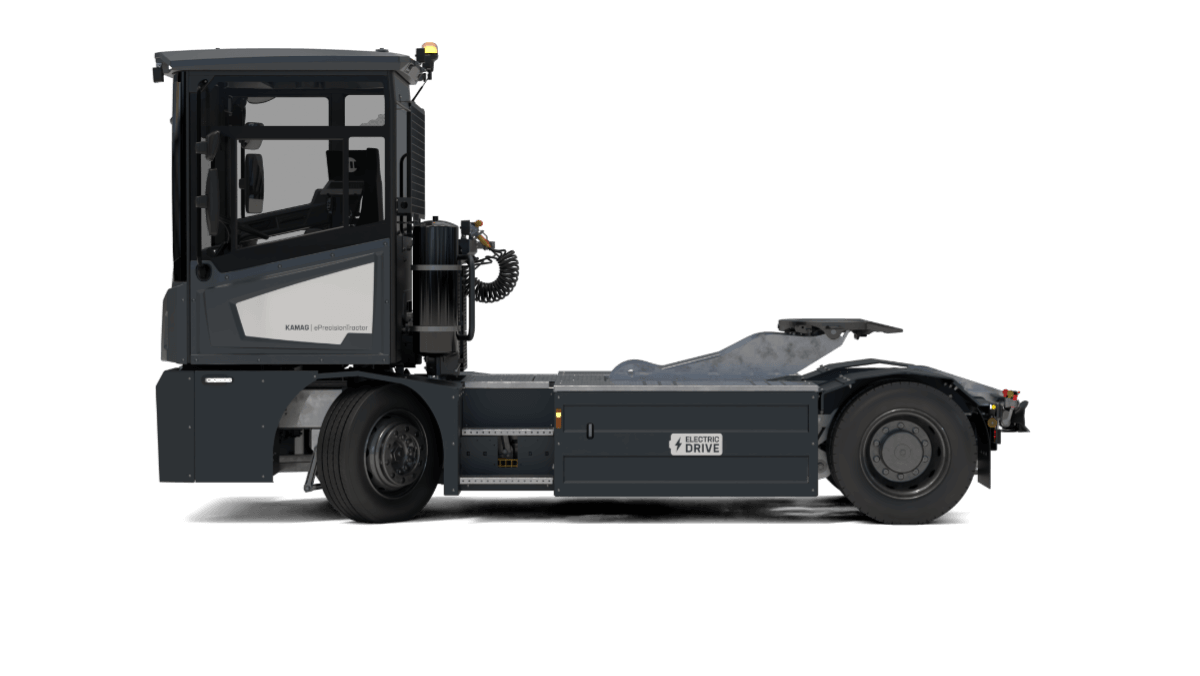
\includegraphics[width=\linewidth]{images/PrecisionTractor.png}
    \captionof{figure}{Kamag Precision Tractor\cite{tiikamag_website}}
        \label{fig:precision_tractor}
  \end{minipage}
    \hfill
  \begin{minipage}{0.4\textwidth}
        \centering
        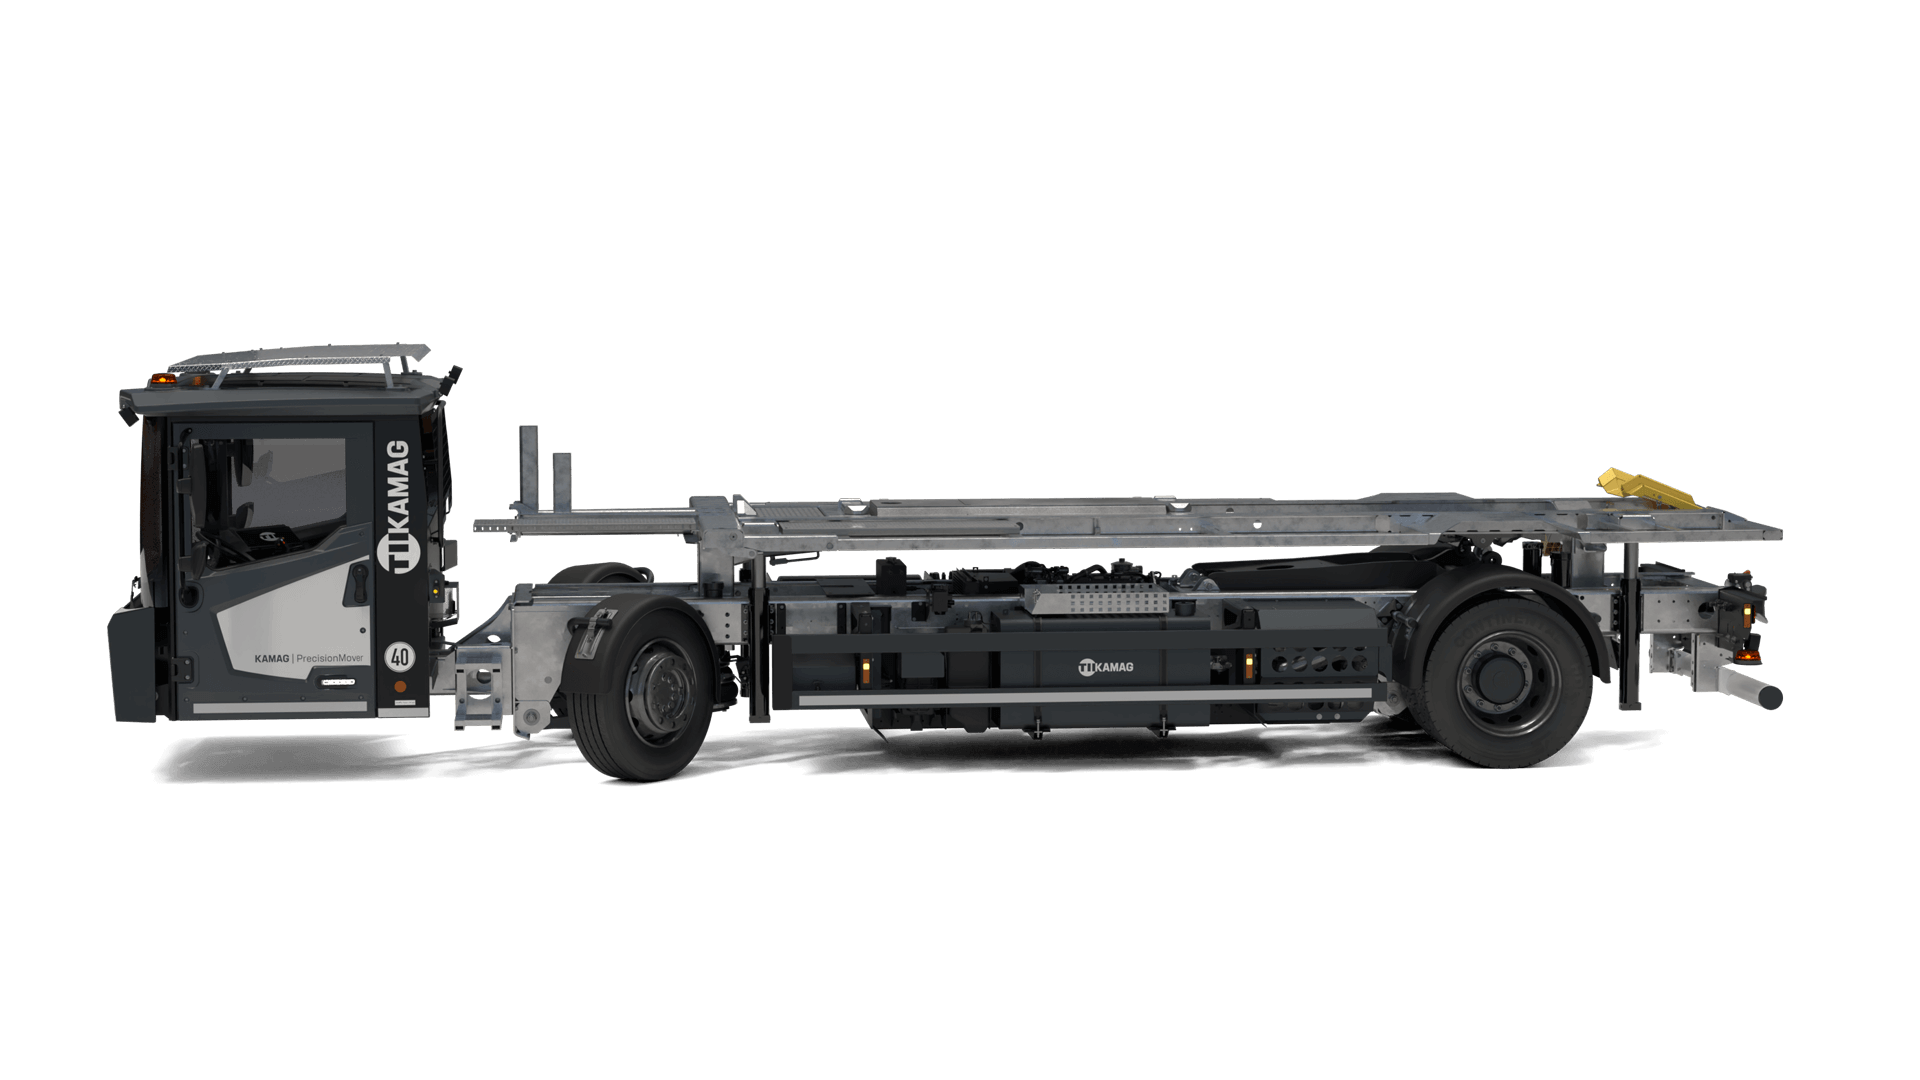
\includegraphics[width=\linewidth]{images/PrecisionMover.png}
    \captionof{figure}{Kamag Precision Mover\cite{tiikamag_website}}
        \label{fig:precision_mover}
  \end{minipage}

\end{figure}

TII KAMAG operates from an industrial site comprising multiple production facilities and technical departments dedicated to the development of transport technologies. The company employs approximately 350 people who contribute to the design, manufacturing, and continuous improvement of specialized transport solutions for customers worldwide.
\begin{figure}[H]
    \centering
  \begin{minipage}{0.48\textwidth}
        \centering
        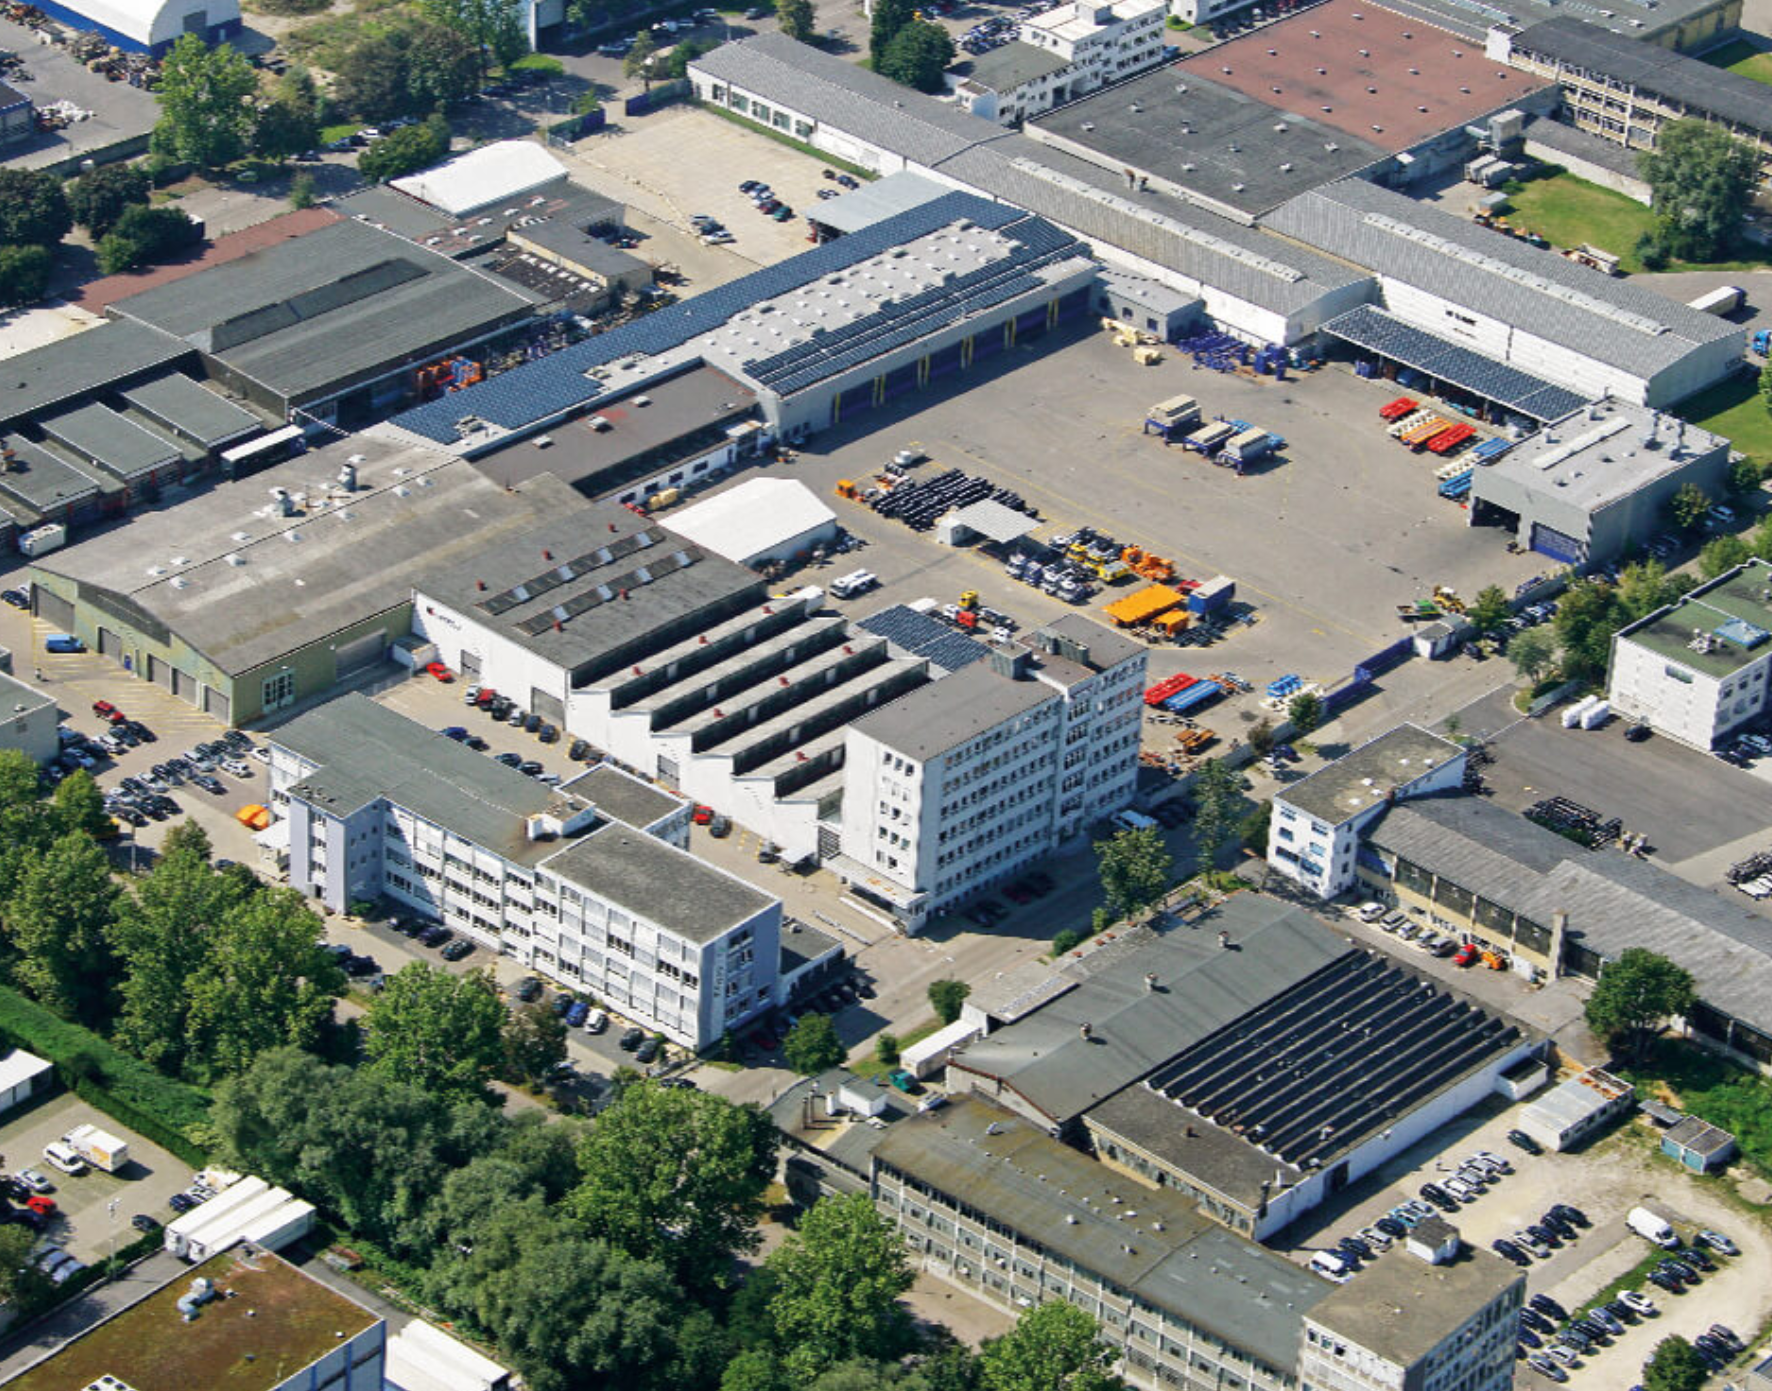
\includegraphics[width=\linewidth]{images/TIIKAMAGYARD.png}  
        \captionof{figure}{TII KAMAG Campus\cite{tiikamag_website}}
        \label{fig:tiikamag_yard}
  \end{minipage}
\end{figure}


\subsection{Project Context and Objectives}

The development of autonomous transport solutions creates a need for suitable methods to evaluate their operational effectiveness. Unlike stationary production equipment, autonomous yard vehicles execute variable transport missions under changing traffic and environmental conditions. These characteristics make the direct application of classical OEE insufficient for identifying and interpreting the main sources of operational loss.

Within this industrial context, the objective of this graduation project is to \textbf{design and implement an \gls{oee}-based performance measurement framework adapted to autonomous yard logistics}. The work aims to define suitable Availability, Performance, and Quality metrics, account for \GLS{odd}-related constraints. It also provides complementary indicators for deeper operational diagnosis. The framework is supported by a structured data model and implemented using the available operational data.

\section{Autonomous Yard-Logistics System}
\label{sec:industrial-operating-context}

The system under study operates within the DACHSER yard, where autonomous vehicles perform swap body transfer operations in a defined industrial logistics area.

\subsection{Operating Environment and System Actors}

The yard is a semi-structured environment with predefined driving paths connecting multiple parking locations. Parking locations may contain swap bodies, standardized load units supported by folding legs, or no load unit. The area is shared with pedestrians and manually operated vehicles, so the autonomous system must navigate intersections, crossing areas, and changing operational conditions.

Three actors are involved in the operation: the autonomous Kamag Precision Mover, which executes transport missions; the remote supervisor or safety operator, who monitors operation, manages protective stops, validates specific manoeuvres, and intervenes when necessary; and the yard operations team, which manages transport orders, mission coordination, and operational exceptions.

\subsection{Swap Body Transfer Workflow}

The transfer is the basic unit of operation and represents the relocation of one swap body from a source location to a destination location. It may involve two missions: a pick-up mission, during which the Kamag Precision Mover travels to the source location, positions itself beneath the swap body, and lifts it; and a set-down mission, during which the loaded vehicle transports the swap body to the destination and unloads it.

\begin{figure}[H]
  \centering
  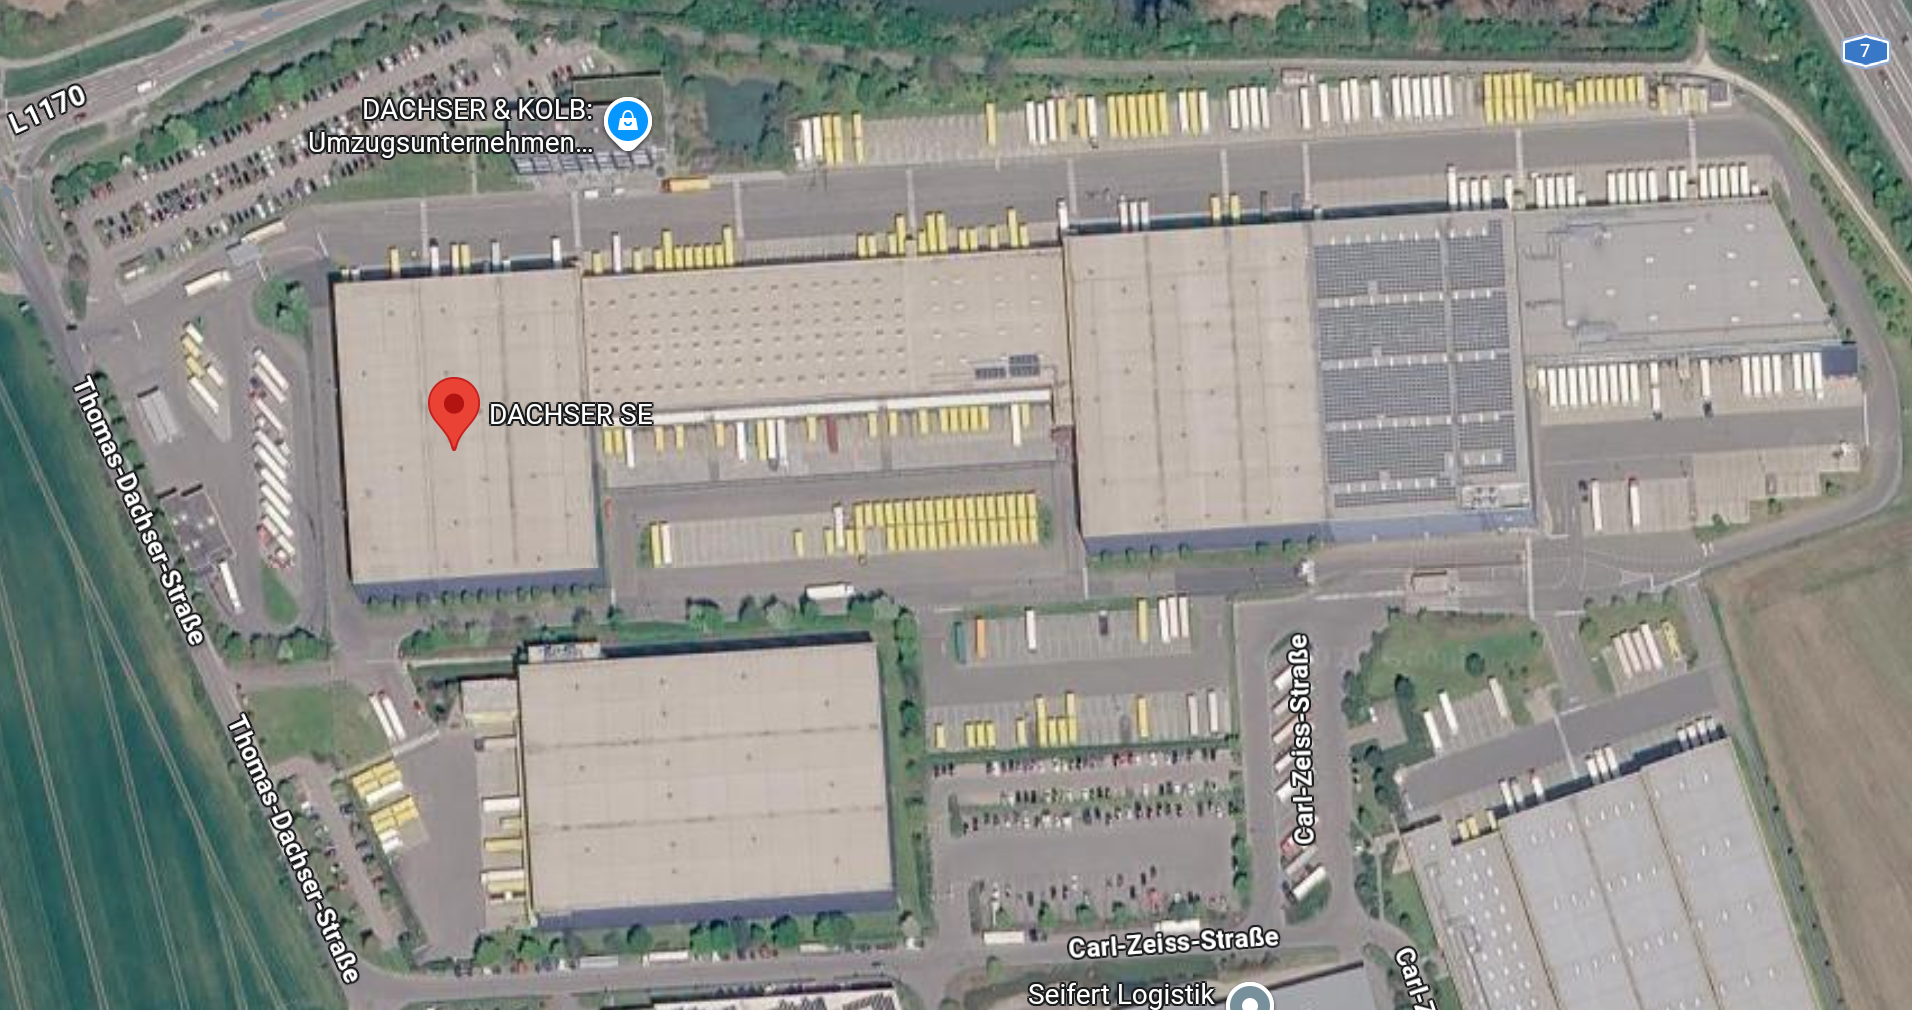
\includegraphics[width=0.7\textwidth]{images/dachseryard.png}
  \caption[The Dachser Yard]{The Dachser Yard~\cite{dachser_google_maps}}
  \label{fig:dachseryard}
\end{figure}
\subsection{Operational Hierarchy}
The logistics operation is structured into three levels: transfer, mission, and mission phase. A transfer represents the complete transport order from a source location to a destination. It is composed of one or two missions depending on the transfer scenario. Each mission describes a specific part of the transport operation, such as pick-up, set-down, or repositioning. Missions are further decomposed into elementary mission phases that describe the individual actions executed by the vehicle.
\subsection{Mission Phases and Transfer Scenarios}

The vehicle operation is divided into eight mission phases, denoted MP1 to MP8. These phases cover path following, manoeuvring, insertion, load handling, extraction, and return to the predefined path. Table \ref{tab:mission-phases} summarises their definitions, while Figure \ref{fig:MPdesc} illustrates the phase sequence.

\begin{figure}[H]
  \centering
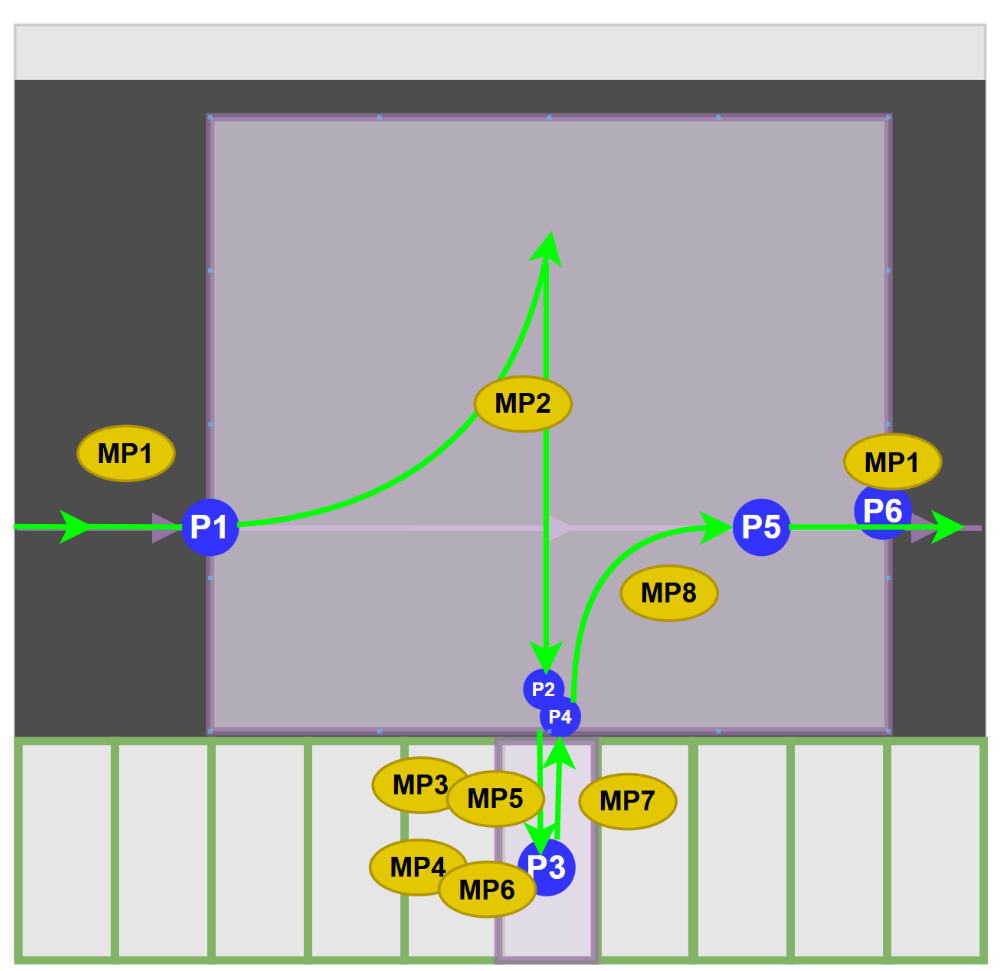
\includegraphics[width=0.7\textwidth]{images/MPdesc.png}
\caption{Mission Phases Representation}
\label{fig:MPdesc}
\end{figure}

\begin{table}[H]
  \centering
  \caption{Canonical Mission Phases}
  \label{tab:mission-phases}
  \begin{adjustbox}{max width=\textwidth}
    \begin{tabular}{|c|p{4.3cm}|c|p{5.8cm}|}
      \hline
      \textbf{Phase} & \textbf{Description} & \textbf{Navigation mode} & \textbf{Detailed description} \\
      \hline
      MP1 & Follow the predefined path & follower & The \gls{av} drives forward or backward along the predefined path to \textbf{P1} \\
      \hline
      MP2 & Manoeuvre toward pre-insertion point & manoeuvre & From \textbf{P1} to \textbf{P2} \\
      \hline
      MP3 & Insert into spot under swap body & manoeuvre & From \textbf{P2} to \textbf{P3} \\
      \hline
      MP4 & Pick up swap body & manoeuvre & At \textbf{P3} \\
      \hline
      MP5 & Insert into empty spot & manoeuvre & From \textbf{P2} to \textbf{P3} \\
      \hline
      MP6 & Set down swap body & manoeuvre & At \textbf{P3} \\
      \hline
      MP7 & Extract from spot & manoeuvre & From \textbf{P3} to \textbf{P4} \\
      \hline
      MP8 & Catch up the predefined path & manoeuvre & From \textbf{P4} to \textbf{P5} \\
      \hline
    \end{tabular}
  \end{adjustbox}
\end{table}

A transfer is classified by whether each of its two missions requires long-distance travel or takes place in close proximity to the target spot:

\begin{table}[H]
  \centering
  \caption{Transfer scenarios}
  \label{tab:transfer-scenarios}
  \renewcommand{\arraystretch}{1.2}
  \begin{tabular}{|p{3cm}|p{11cm}|}
      \hline
      \textbf{Scenario} & \textbf{Mission-phase sequence} \\
      \hline
      \textbf{classic} &
      \parbox[t]{\linewidth}{\textbf{Mission 1: PICK\_UP}\\ MP7 $\rightarrow$ MP8 $\rightarrow$ MP1 $\rightarrow$ MP2 $\rightarrow$ MP3 $\rightarrow$ MP4\\[0.2em]
      \textbf{Mission 2: SET\_DOWN}\\ MP7 $\rightarrow$ MP8 $\rightarrow$ MP1 $\rightarrow$ MP2 $\rightarrow$ MP5 $\rightarrow$ MP6} \\
      \hline
      \textbf{Close proximity pick up} &
      \parbox[t]{\linewidth}{\textbf{Mission 1: CLOSE\_PROXIMITY\_PICK\_UP}\\ MP7 $\rightarrow$ MP2 $\rightarrow$ MP3 $\rightarrow$ MP4\\[0.2em]
      \textbf{Mission 2: SET\_DOWN}\\ MP7 $\rightarrow$ MP8 $\rightarrow$ MP1 $\rightarrow$ MP2 $\rightarrow$ MP5 $\rightarrow$ MP6} \\
      \hline
      \textbf{Close proximity set down} &
      \parbox[t]{\linewidth}{\textbf{Mission 1: PICK\_UP}\\ MP7 $\rightarrow$ MP8 $\rightarrow$ MP1 $\rightarrow$ MP2 $\rightarrow$ MP3 $\rightarrow$ MP4\\[0.2em]
      \textbf{Mission 2: CLOSE\_PROXIMITY\_SET\_DOWN}\\ MP7 $\rightarrow$ MP2 $\rightarrow$ MP5 $\rightarrow$ MP6} \\
      \hline
      \textbf{Double close proximity} &
      \parbox[t]{\linewidth}{\textbf{Mission 1: CLOSE\_PROXIMITY\_PICK\_UP}\\ MP7 $\rightarrow$ MP2 $\rightarrow$ MP3 $\rightarrow$ MP4\\[0.2em]
      \textbf{Mission 2: CLOSE\_PROXIMITY\_SET\_DOWN}\\ MP7 $\rightarrow$ MP2 $\rightarrow$ MP5 $\rightarrow$ MP6} \\
      \hline
      \textbf{park (GO\_TO)} &
      \parbox[t]{\linewidth}{\textbf{Mission 1: GO\_TO}\\ MP7 $\rightarrow$ MP8 $\rightarrow$ MP1 $\rightarrow$ MP2 $\rightarrow$ MP5\\[0.2em]
      \textit{Single mission scenario}} \\
      \hline
    \end{tabular}
  \renewcommand{\arraystretch}{0.85}
\end{table}

\subsection{System and Data Architecture}

The autonomous yard logistics system consists of two layers: an onboard vehicle layer and an off-board data-management layer. During transport missions, the \gls{av} continuously generates data on vehicle states, mission execution, events, and outcomes.

At the vehicle level, onboard logging records each mission's operational trace, including timestamps, mission phases, system events, and execution results. These records support the reconstruction of transport operations and the identification of performance losses.

The telemetry data is transmitted to off-board systems, where fleet information is consolidated into an Automatic Telemetry Dataset. This dataset provides the main input for computing \glspl{kpi} and evaluating \gls{oee}.

This architecture links autonomous operation to performance analysis: vehicle execution generates operational data, telemetry systems collect and organize it, and the resulting dataset supports the evaluation of autonomous yard effectiveness.
\begin{figure}[H]
  \centering
  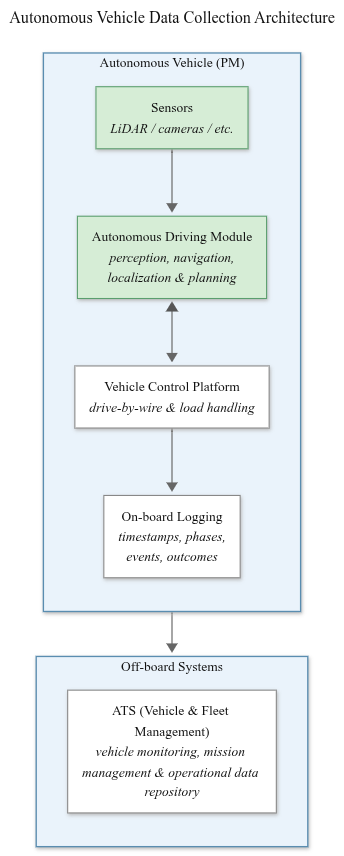
\includegraphics[width=0.3\textwidth]{images/System Architecture.png}
  \caption{System Architecture}
  \label{fig:systemarchitecture}
\end{figure}

\subsection{Available Data and Evaluation Constraints}

This section describes the data foundation used to design and evaluate the proposed performance measurement framework.
\begin{itemize}
  \item \textbf{Data sources:} The framework relies on two complementary data sources. The first is the automatic dataset, generated from vehicle operation and containing machine-recorded information such as timestamps, mission phases, operational events, and execution outcomes. The second is a manual field log maintained by operators, providing additional contextual information regarding interventions, exceptions, and operational events that cannot always be fully captured through automatic telemetry alone. These two sources are combined at the transfer level to create a unified structured dataset representing each transport operation. Real operational data from both sources was analysed during the design phase to identify the data fields and input structure required by the proposed framework, and to validate that the necessary information is practically collectable from the system.


  \item \textbf{Historical and synthetic data:} Due to limitations in data coverage and completeness, real records alone were insufficient for a comprehensive evaluation. A synthetic dataset was therefore generated following the same input schema derived from the real data, enabling controlled and reproducible testing of the framework under predefined performance scenarios while remaining consistent with real operational characteristics.
\end{itemize}
\begin{figure}[H]
  \centering
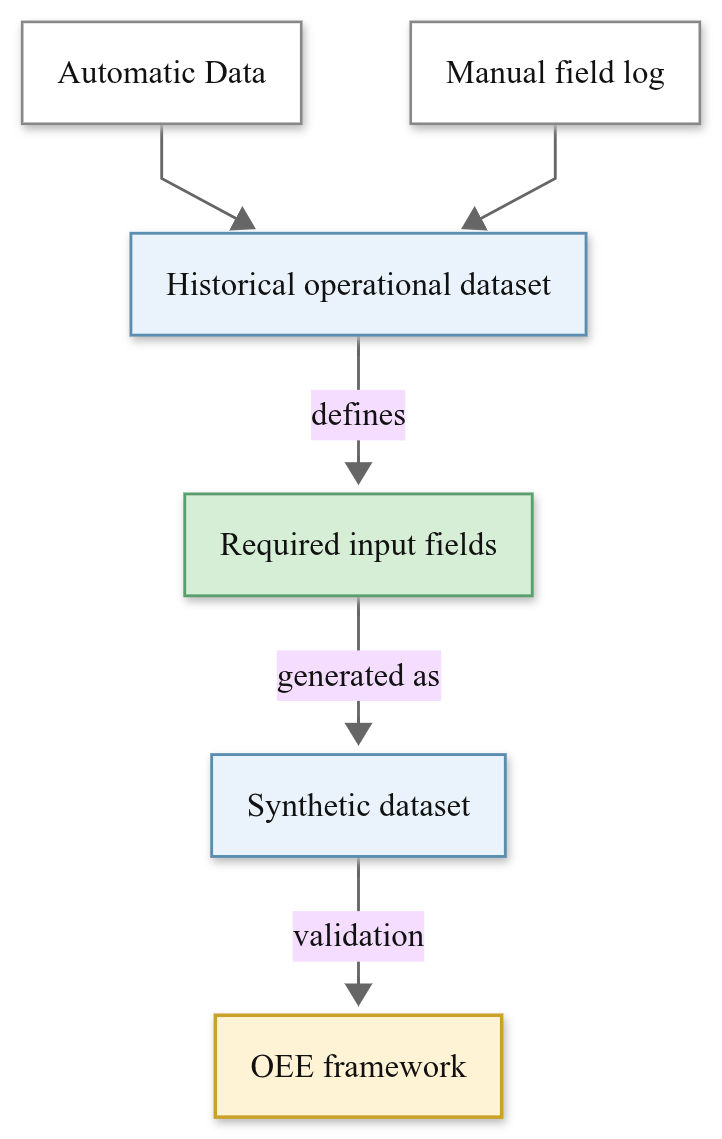
\includegraphics[width=0.4\textwidth]{images/Data provenance flow.png}
\caption{Data Provenance Flow}
\label{fig:datacollectioncontext}
\end{figure}


\section{Industrial Performance-Measurement Problem}

\gls{oee} was developed to evaluate stationary manufacturing equipment operating under repetitive and predictable conditions. Its classical formulation assumes fixed production cycles, clearly defined operating states, and losses categorized as availability, performance, and quality. Under these conditions, \gls{oee} effectively measures equipment utilization and production efficiency.

These assumptions do not fully apply to \glspl{av} operating in dynamic yard environments. Unlike industrial machines, \gls{av} missions are affected by travel distances, route configurations, traffic, loading and unloading operations, and interactions with people and infrastructure. Operational interruptions also cannot always be interpreted as equipment failures. An \gls{av} may stop because of safety constraints, remote-supervision requests, autonomy limitations, congestion, or environmental conditions while remaining technically functional.

Applying conventional \gls{oee} to autonomous yard operations may therefore obscure the true causes of performance losses by grouping fundamentally different events into identical categories. Mechanical failures, autonomy-related limitations, safety interventions, and environmental constraints require separate interpretation to support effective operational decisions.

Current autonomous-driving metrics, such as disengagement rate and intervention frequency, primarily evaluate autonomy and safety. However, they do not measure the overall effectiveness of logistics operations. Traditional \gls{oee}, measures equipment efficiency but lacks the operational states and loss categories required for autonomous vehicles. This creates a measurement gap: existing approaches cannot precisely determine the useful transport work performed by an autonomous fleet.

A dedicated performance-measurement framework is therefore required for autonomous yard logistics. Such a framework should preserve the industrial relevance of \gls{oee} while adapting its time hierarchy, performance indicators, and loss classification to mission variability, autonomy-specific events, supervision requirements, and operational constraints. This work addresses this need by developing an \gls{oee}-based performance-measurement approach for the autonomous transport system deployed in the DACHSER yard.

\section{Overall Equipment Effectiveness Foundations}

This section presents the foundations of \gls{oee} and its relevance to autonomous yard logistics. It reviews the classical \gls{oee} framework, its extension beyond manufacturing, and the assumptions underlying its main factors. It also introduces the Six Big Losses and relevant industrial standards. These foundations provide the basis for identifying the limitations that motivate the adapted framework proposed in this work.
\subsection{Origins and Rationale of OEE}
 \gls{oee} is a key manufacturing metric used to quantify production efficiency by identifying and reducing operational losses. Seiichi Nakajima introduced the concept in 1988 as part of Total Productive Maintenance (\gls{tpm}), a methodology developed by the Japan Institute of Plant Maintenance.\cite{nakajima1988tpm} The objective of \gls{tpm} is to maximize equipment effectiveness throughout its lifecycle through a comprehensive maintenance system involving all departments and employees.

Nakajima's work provided a structured method for evaluating equipment performance beyond simple uptime. OEE combines equipment availability, operating speed, and product quality to reveal the capacity lost through inefficiencies. This lost capacity is often described as the ``Hidden Factory.'' By separating overall effectiveness into distinct factors, OEE supports targeted improvement actions and waste reduction.
\subsection{Availability, Performance, and Quality}
OEE is calculated as the product of three factors:
\[
\mathrm{OEE} = A \cdot P \cdot Q
\]
Availability, Performance, and Quality represent different types of operational loss:
\begin{itemize}
    \item \textbf{Availability} measures the proportion of scheduled operating time during which the equipment is running. It accounts for downtime losses such as breakdowns, setups, and adjustments.
    \item \textbf{Performance} compares the actual operating speed with the ideal cycle time. It accounts for losses caused by minor stops and reduced speed.
    \item \textbf{Quality} measures the proportion of good products in the total output. It accounts for losses caused by defects and rework.
\end{itemize}
\subsection{Fixed-Cycle Assumption}
Classical OEE relies on a fixed-cycle assumption. For a given product, the ideal production cycle is assumed to remain constant. This cycle provides the reference for measuring actual operating speed and calculating the Performance factor. Deviations from the ideal cycle, including minor stops and reduced speed, are therefore classified as performance losses.

This assumption is effective in stable and repetitive manufacturing environments. However, it becomes difficult to apply to dynamic systems whose mission durations and operating conditions vary. This limitation is particularly important when extending OEE to autonomous vehicles.
\subsection{The Six Big Losses}
Nakajima's OEE framework classifies production inefficiencies into the ``Six Big Losses.''\cite{nakajima1988tpm} This taxonomy provides a structured method for identifying the main causes of equipment underutilization:
\begin{enumerate}
    \item \textbf{Equipment Failure (Availability Loss):} unplanned downtime caused by breakdowns or technical faults.
    \item \textbf{Setup and Adjustment (Availability Loss):} planned downtime required to prepare the machine for a different production run.
    \item \textbf{Idling and Minor Stops (Performance Loss):} brief interruptions or jams that temporarily stop production.
    \item \textbf{Reduced Speed (Performance Loss):} operation at a speed below the theoretical maximum.
    \item \textbf{Process Defects (Quality Loss):} scrap or defective parts produced during steady-state operation.
    \item \textbf{Reduced Yield (Quality Loss):} defective parts produced during startup or production transitions.
\end{enumerate}
The Six Big Losses are highly effective for static and repetitive manufacturing processes because they provide a clear structure for continuous improvement. However, their direct application to autonomous yard logistics requires adaptation to mobile operation, variable missions, and autonomy-related events.
\begin{figure}[H]
   \centering
  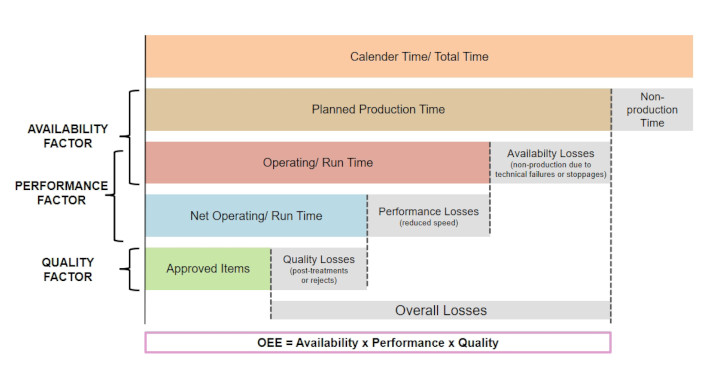
\includegraphics[width=0.8\textwidth]{images/Time-model-for-OEE-measuring.jpg}
  \caption[Major Losses and Computation of OEE]{Major Losses and Computation of OEE\cite{sciencedirect_oee_figure}}
  \label{fig:hard}
\end{figure}
\subsection{Industrial Standards and Guidelines}
Several standards and industrial guidelines support the consistent definition and measurement of OEE-related indicators:
\begin{itemize}
  \item \textbf{ISO 22400-2:2014:} This standard defines KPIs for manufacturing operations management. It provides formal definitions for indicators such as Availability, which is calculated as the ratio of Operating Time to Planned Production Time.\cite{iso22400_2_2014}

  \item \textbf{SEMI E10:} Developed for the semiconductor industry, this standard defines equipment states and provides a framework for measuring reliability, availability, and maintainability (\gls{ram}). It distinguishes states such as Productive, Standby, and Unscheduled Downtime.\cite{semi_e10_ram} SEMI E79 extends this framework to define OEE for semiconductor manufacturing equipment.

  \item \textbf{VDMA guidelines:} Guidelines such as VDMA 66412 support the standardization of manufacturing execution system (\gls{mes}) KPIs. They are generally aligned with ISO 22400 and provide guidance for data collection and analysis, with particular emphasis on technical availability.
\end{itemize}
\section{OEE Beyond Manufacturing}
While OEE originated in discrete manufacturing, its underlying principles of identifying, classifying, and quantifying operational losses have gradually been extended to other industrial domains. As automation has expanded beyond traditional production lines, researchers have explored the application of OEE to logistics, warehousing, and mobile robotic systems. Although the fundamental objective remains the maximization of asset effectiveness, the transition from stationary production equipment to mobile autonomous systems requires substantial adaptation of both performance indicators and loss definitions.
\subsection{OEE in Logistics and Material-Handling Systems}
The application of OEE has progressively expanded from manufacturing equipment to automated material handling systems, including conveyor systems, sorting equipment, \glspl{agv}, and \glspl{amr}. These technologies play an increasingly important role in modern intralogistics by automating material transportation and improving operational efficiency.

\subsection{Adaptation of OEE Components to Mobile Systems}
Existing research shows that the three classical OEE dimensions remain applicable to mobile robotic systems, but require reinterpretation. Availability reflects vehicle readiness and downtime, Performance focuses on mission execution efficiency and speed, and Quality considers successful and error-free mission completion. Thus, OEE shifts from measuring machine productivity to evaluating the effectiveness and utilization of autonomous material handling systems~\cite{fragapane2021intralogistics}.
\begin{figure}[H]
   \centering
  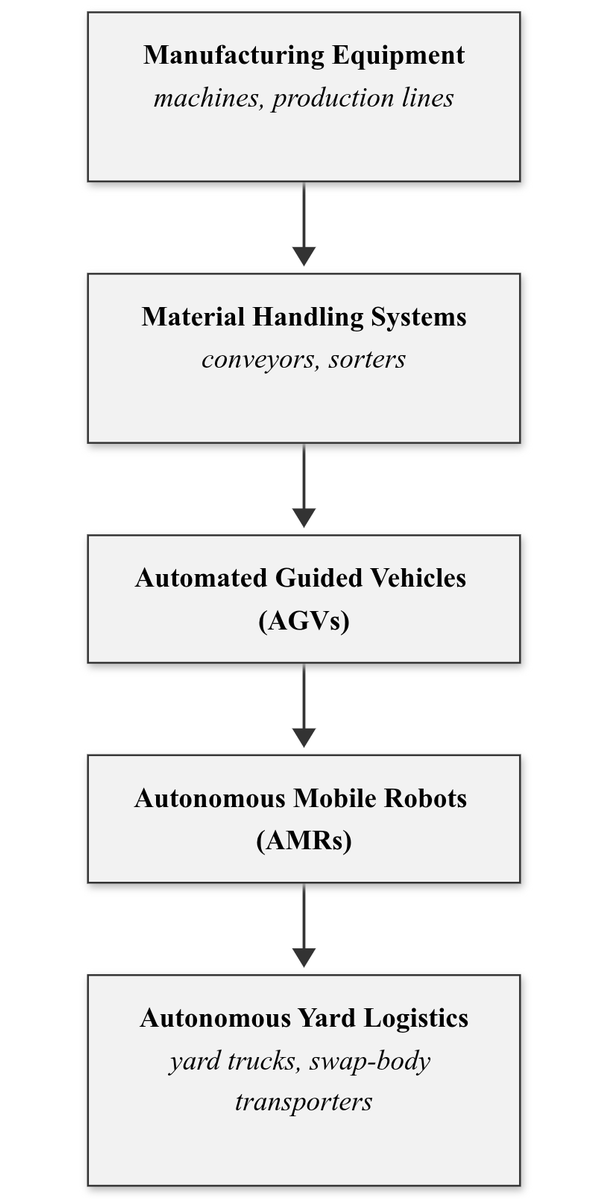
\includegraphics[width=0.3\textwidth]{images/oee_evolution.png}
  \caption[Evolution of OEE applications]{Evolution of OEE applications in logistics and mobile robotic systems.}
  \label{fig:oee-evolution}
  
\end{figure}
\subsection{Adaptation of the Six Big Losses}
Applying \gls{oee} to mobile logistics also requires reinterpreting Nakajima's Six Big Losses. The original loss taxonomy was developed for stationary production equipment. Therefore it does not adequately represent the operational characteristics of autonomous mobile systems operating in dynamic environments.

Within \glspl{agv} and \glspl{amr} applications, traditional setup and adjustment losses are commonly associated with battery refueling, software updates, vehicle initialization, or task assignment procedures. Idling and minor stoppages are frequently caused by obstacle avoidance, traffic congestion, waiting at intersections, or temporary interactions with human operators. Reduced speed losses arise when vehicles intentionally decrease their speed due to safety constraints, congestion, or navigation requirements. Likewise, process defects are reinterpreted as failed missions, misplaced loads, delivery inaccuracies, or navigation errors requiring manual intervention or mission repetition.

These adaptations demonstrate that although the philosophy of loss identification remains applicable, the nature of the losses changes significantly when moving from fixed manufacturing equipment to autonomous mobile systems. Consequently, several studies emphasize the need for specialized loss taxonomies that accurately represent the operational behavior of autonomous logistics vehicles.
\begin{table}[!ht]
\renewcommand{\arraystretch}{1.5}
\centering
\caption{Adaptation of Nakajima's Six Big Losses to Mobile Logistics}
\label{tab:mobile-logistics-losses}
\begin{tabular}{|p{5cm}|p{9cm}|}
\hline
\textbf{Classical Six Big Loss} & \textbf{Mobile Logistics Interpretation} \\
\hline
Equipment failures & Vehicle hardware or software failures \\
\hline
Setup and adjustment & Battery refueling, software updates, vehicle initialization, task assignment \\
\hline
Idling and minor stops & Obstacle avoidance, traffic congestion, waiting at intersections or doors \\
\hline
Reduced speed & Speed reduction due to safety constraints, congestion, or navigation \\
\hline
Process defects & Failed missions, misplaced loads, delivery errors, navigation failures \\
\hline
Startup losses & Localization, calibration, or system initialization errors \\
\hline
\end{tabular}
\end{table}
\subsection{Limitations of OEE for Autonomous Systems}

Despite these adaptations, applying classical \gls{oee} directly to autonomous systems remains challenging, particularly in outdoor logistics environments. Autonomous vehicles differ from conventional manufacturing equipment in several ways, which complicates the interpretation of the traditional \gls{oee} factors.

First, autonomous vehicles operate in changing environments affected by traffic, weather, pedestrians, and interactions with other vehicles. Unlike production machines operating under controlled conditions, variations in mission duration may result from environmental conditions rather than equipment inefficiency.

Second, the fixed-cycle assumption of classical \gls{oee} is difficult to apply. Mission durations vary with travel distance, route complexity, traffic, obstacle avoidance, and operational priorities. As a result, defining a single ideal cycle time as a meaningful performance benchmark is difficult.

Finally, autonomous systems generate operational events that have no direct equivalent in conventional manufacturing. Human interventions, remote-operator takeovers, disengagements, and autonomous decision-making failures represent additional loss categories that the traditional \gls{oee} framework does not adequately capture. These events affect operational effectiveness and must therefore be considered when adapting \gls{oee} to autonomous vehicles.
\section{Performance Measurement of Autonomous Vehicles}
Evaluating autonomous vehicles requires a broader perspective than traditional indicators such as speed, fuel consumption, and travel distance. In industrial environments, performance depends on the vehicle's ability to execute assigned missions safely, reliably, and efficiently.

Unlike conventional vehicles, autonomous systems depend on the interaction between perception, decision-making, navigation, and environmental conditions. Evaluation therefore requires several frameworks and \glspl{kpi} covering autonomy, safety, reliability, and operational effectiveness.
\subsection{Levels of Driving Automation}
The SAE J3016 standard defines six levels of driving automation, ranging from Level 0 (no automation) to Level 5 (full automation). These levels describe how driving tasks are distributed between the human driver and the automated driving system.

Level 4 automation is particularly relevant to autonomous yard logistics. At this level, the \gls{ads} performs all driving tasks without human intervention within a defined \gls{odd}. Level 4 systems are therefore suitable for controlled industrial environments such as logistics yards, where operating conditions can be constrained and monitored.
\begin{figure}[H]
   \centering
  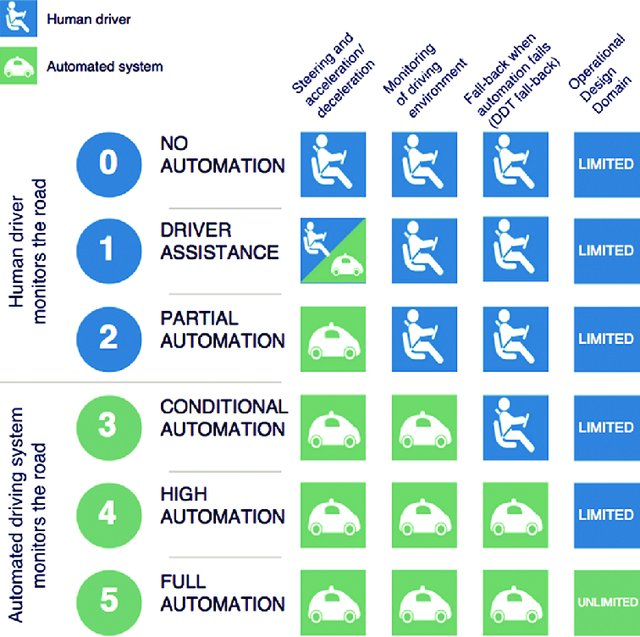
\includegraphics[width=0.4\textwidth]{images/SAE-J3016-levels-of-driving-automation_W640.jpg}
  \caption[SAE Automation Levels]{SAE Automation Levels~\cite{sae_j3016_rg}}
  \label{fig:sae-levels}
  
\end{figure}
\subsection{Autonomous-Vehicle Performance Metrics}
Autonomous vehicles are commonly evaluated using multiple \glspl{kpi}, each addressing a specific aspect of system behaviour. Unlike manufacturing systems, which often use \gls{oee} as an integrated measure of effectiveness, autonomous-vehicle research generally uses separate metrics for autonomy, safety, reliability, and operational efficiency.

Existing review studies indicate that no universally accepted framework comprehensively evaluates autonomous-vehicle performance. Most available metrics focus on individual dimensions rather than overall operational effectiveness. The main metrics used in this context are summarized in Table~\ref{tab:av-performance-metrics}.
\begin{table}[H]
\renewcommand{\arraystretch}{1.5}
\centering
\caption{Common Performance Metrics for Autonomous Vehicles}
\label{tab:av-performance-metrics}
\begin{tabular}{|p{3cm}|p{6cm}|p{5cm}|}
\hline
\textbf{KPI} & \textbf{Description} & \textbf{Performance Aspect} \\
\hline
Mission Success Rate & Percentage of missions completed successfully without failure & Mission effectiveness \\
\hline
Intervention / Disengagement Rate & Frequency of human intervention or autonomous disengagement & Autonomy and reliability \\
\hline
Technical Availability & Percentage of time the vehicle is operationally ready & System readiness \\
\hline
Mission Cycle Time & Time required to complete a transport mission & Operational efficiency \\
\hline
Fleet Utilization & Percentage of vehicles actively performing missions & Asset utilization \\
\hline
\end{tabular}
\end{table}
\subsection{Operational Design Domain}
The \gls{odd} defines the conditions under which an \gls{ads} is designed to operate safely and effectively. It describes the limits of the system's operational capability. These limits depend on environmental and operational factors. They also determine when autonomous operation can continue without human intervention.

For autonomous yard vehicles, the \gls{odd} specifies the areas in which the vehicle can operate. It also defines the conditions required for autonomous operation. These conditions include the infrastructure, road layout, weather, lighting, traffic, and presence of dynamic obstacles. They may also include speed restrictions, visibility requirements, and interaction with pedestrians or manually operated vehicles.
\subsection{ODD, SOTIF, and Performance Measurement}
ISO 34503 provides a structured approach for describing the \gls{odd} of automated driving systems. It organizes ODD characteristics into categories such as scenery, environmental conditions, and dynamic elements~\cite{iso34503_2023}.

Figure~\ref{fig:odd-components} illustrates these ODD components. Together, they define the context in which an automated driving system must operate safely. A change in any of these components may affect the vehicle's ability to continue autonomous operation.

\begin{figure}[H]
   \centering
  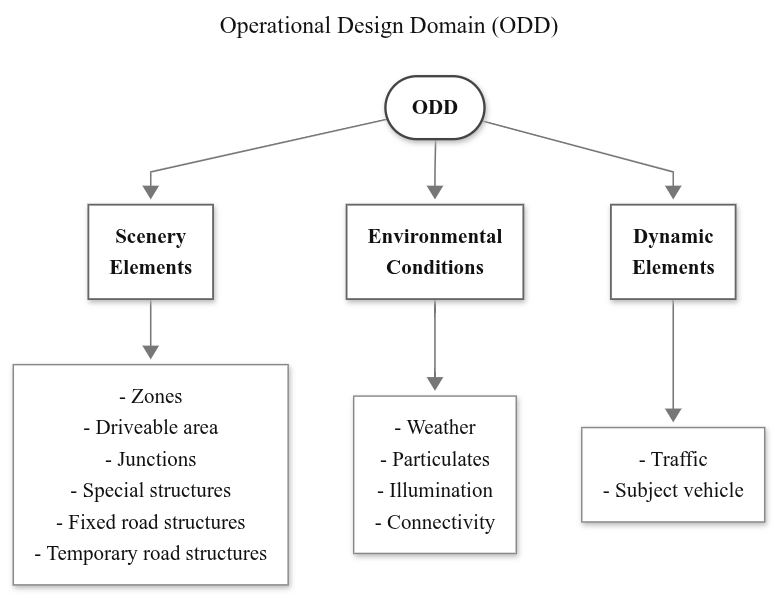
\includegraphics[width=0.6\textwidth]{images/odd_components.png}
  \caption[ODD Components]{Operational Design Domain Components~\cite{iso34503_2023}}
  \label{fig:odd-components}
\end{figure}

The \gls{sotif} concept, defined by ISO 21448, addresses safety risks caused by functional limitations of an automated system rather than hardware failures~\cite{iso21448_2022}. This concept is important for autonomous vehicles operating in complex environments, where unexpected situations may occur even when the hardware remains functional.

For example, fog or other conditions that reduce visibility may prevent an autonomous vehicle from continuing safely despite the correct operation of its hardware components.


The distinction between \gls{odd} exclusions and technical failures is therefore important. A technical failure occurs when a system component does not operate as intended, such as in the case of a sensor malfunction, communication failure, or software error. An \gls{odd} exclusion occurs when the vehicle encounters conditions outside its defined operational boundaries, such as heavy rain, dense fog, or insufficient visibility. In this case, the vehicle may remain technically functional but unable to continue autonomous operation.

This distinction affects the adaptation of \gls{oee} to autonomous vehicles. In conventional manufacturing, Availability losses are mainly associated with equipment breakdowns, maintenance, and setup activities. Autonomous vehicles introduce additional sources of unavailability related to environmental and operational constraints. ODD exclusions should therefore be treated as a distinct category of operational loss when evaluating the Availability factor.
\section{Complementary Performance Indicators}
Although OEE provides a holistic measure of operational effectiveness through the integration of Availability, Performance, and Quality, it does not fully characterize all aspects of autonomous system behaviour. In particular, reliability engineering metrics provide insight into failure behaviour and maintainability, while statistical quality methods allow the evaluation of operational consistency and variability.
\subsection{Reliability and Maintainability Metrics}
\label{sec:reliability_state_art}
Reliability engineering provides established methods for evaluating the robustness and maintainability of complex systems. For autonomous vehicles, these metrics are particularly relevant because operational effectiveness depends not only on task execution but also on the ability of the system to remain available and recover from failures.

The main reliability indicators include:

\begin{itemize}
  \item \textbf{Failure Rate ($\lambda$):} represents the frequency at which failures occur during operation. For systems with an approximately constant failure rate, it is commonly related to \gls{mtbf} as:
\end{itemize}

\[
\lambda = \frac{1}{\mathrm{MTBF}}
\]

\begin{itemize}
  \item \textbf{\gls{mtbf}:} represents the average operating time between two consecutive failures. A higher \gls{mtbf} indicates improved reliability and fewer interruptions caused by system faults.
  \item \textbf{\gls{mttr}:} represents the average time required to restore the system after a failure. A lower \gls{mttr} indicates improved maintainability and faster recovery.
\end{itemize}

These reliability indicators can be combined to estimate technical availability:

\[
A = \frac{\mathrm{MTBF}}{\mathrm{MTBF} + \mathrm{MTTR}}
\]

This availability definition describes the proportion of time that a system is operational from a reliability perspective. It directly relates to the Availability component of OEE; however, the two concepts are not identical. Reliability-based availability focuses on the technical state of the system, while OEE Availability considers whether the asset is available for productive operation within the planned production or operational period.
\subsection{Process Capability}
Process capability indices $C_p$ and $C_{pk}$ are statistical measures used to evaluate how well a process operates within predefined specification limits~\cite{six_sigma_cp_cpk}. For a process characteristic with lower and upper specification limits (\gls{lsl} and \gls{usl}), process mean $\mu$, and standard deviation $\sigma$, the capability indices are defined as:

\[
C_p = \frac{\mathrm{USL} - \mathrm{LSL}}{6\sigma}
\]

\[
C_{pk} = \min\left(\frac{\mathrm{USL} - \mu}{3\sigma}, \frac{\mu - \mathrm{LSL}}{3\sigma}\right)
\]

The $C_p$ index represents the potential capability of a process by evaluating the ratio between the allowed specification range and the natural process variability. However, it assumes that the process is perfectly centred. The $C_{pk}$ index additionally considers the deviation of the process mean from the target value and therefore provides a more realistic evaluation of the actual process capability.

In the context of autonomous yard logistics, capability analysis provides complementary information to OEE by addressing the variability of execution performance. While OEE Performance evaluates the loss between actual and ideal execution rates, $C_p$ and $C_{pk}$ quantify the consistency with which repeated operations remain within an expected execution-time range. Therefore, capability analysis directly relates to the fixed-cycle assumption discussed earlier in this chapter, as it evaluates how closely actual mission durations follow the nominal cycle time. This aspect is particularly relevant for autonomous systems, where execution times may vary due to traffic interactions, obstacle avoidance, and dynamic operational conditions.

\section{Research Gap and Project Positioning}

The literature review shows that existing approaches provide valuable tools for evaluating industrial and autonomous systems; however, several limitations remain when applying them to autonomous yard logistics.

Classical OEE was developed for stable manufacturing environments with repetitive operations and predefined cycle times. Its direct application to autonomous vehicles is challenging due to variable mission durations caused by traffic interactions, obstacle avoidance, environmental conditions, and operational constraints. Therefore, the \textbf{fixed-cycle assumption underlying the traditional Performance factor requires adaptation}.

Furthermore, autonomous vehicle evaluation relies on multiple \glspl{kpi}, such as mission success rate, intervention rate, technical availability, and fleet utilization. While these metrics assess specific aspects of operation, they are generally considered independently and do not provide an integrated measure combining availability, performance, and quality losses.

Autonomous systems also introduce new sources of operational unavailability. In particular, \textbf{\gls{odd}-related limitations must be distinguished from technical failures}, as a vehicle may remain functional but unable to operate under certain environmental conditions. Such losses are not explicitly represented in classical OEE frameworks.

Additionally, reliability metrics (\gls{mtbf}, \gls{mttr}) and capability indices ($C_p$ and $C_{pk}$) provide complementary information regarding system robustness and execution-time consistency, but they are rarely integrated with OEE for autonomous logistics applications.


%To visually represent the capabilities of the NOVA Operations Platform, its user-friendly interface, and how it integrates various operational aspects into a cohesive system, the following figure from Unisphere's official website can be included:

%\begin{figure}[H]
%  \centering
%  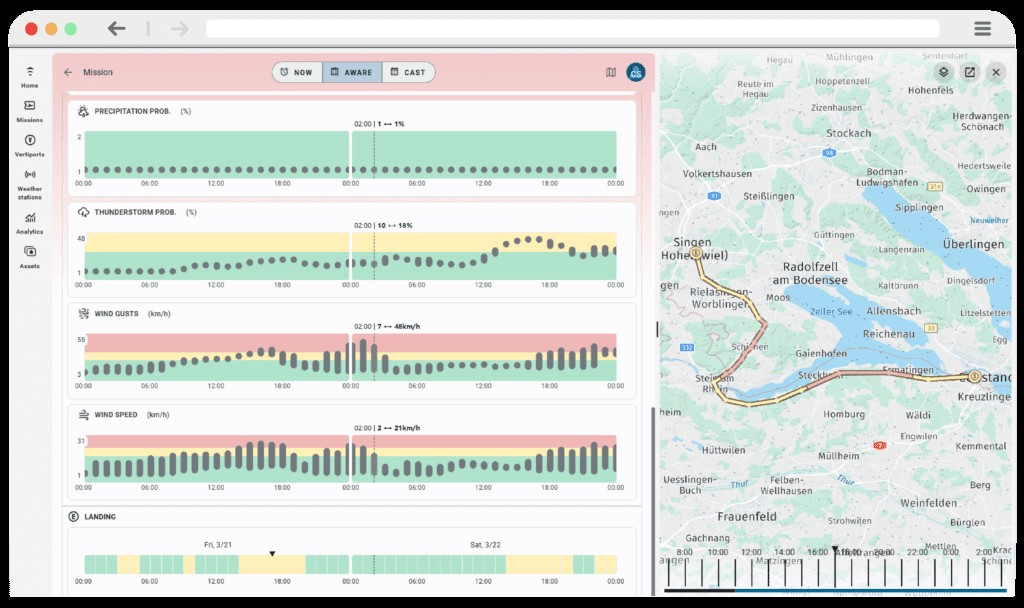
\includegraphics[width=0.9\textwidth]{images/NOVA.jpg}
%  \caption{NOVA Platform interface for mission planning and weather tools.}
%  \label{fig:nova}
%


\section{Project Methodology and Work Plan}

\subsection{Development Approach}

The internship followed a structured yet flexible approach inspired by Agile principles. Rather than relying on a rigid predefined plan, the work progressed incrementally through data analysis, KPI definition, implementation, testing, and validation. Each stage was reviewed and refined based on practical findings and technical feedback.

The first steps focused on understanding the OEE methodology, system architecture, and available data. The work then progressed toward data preparation, KPI computation, validation, and reporting. Regular exchanges with the company supervisor and updates to the academic supervisor ensured continuous alignment with the project objectives.
\subsection{Project Timeline}
The internship spanned a total of six months, from March 2026 to August 2026. The project was divided into clear, consecutive phases to ensure efficient progress and a logical development workflow. The following timeline outlines the major milestones and activities:

\begin{figure}[H]
  \centering
  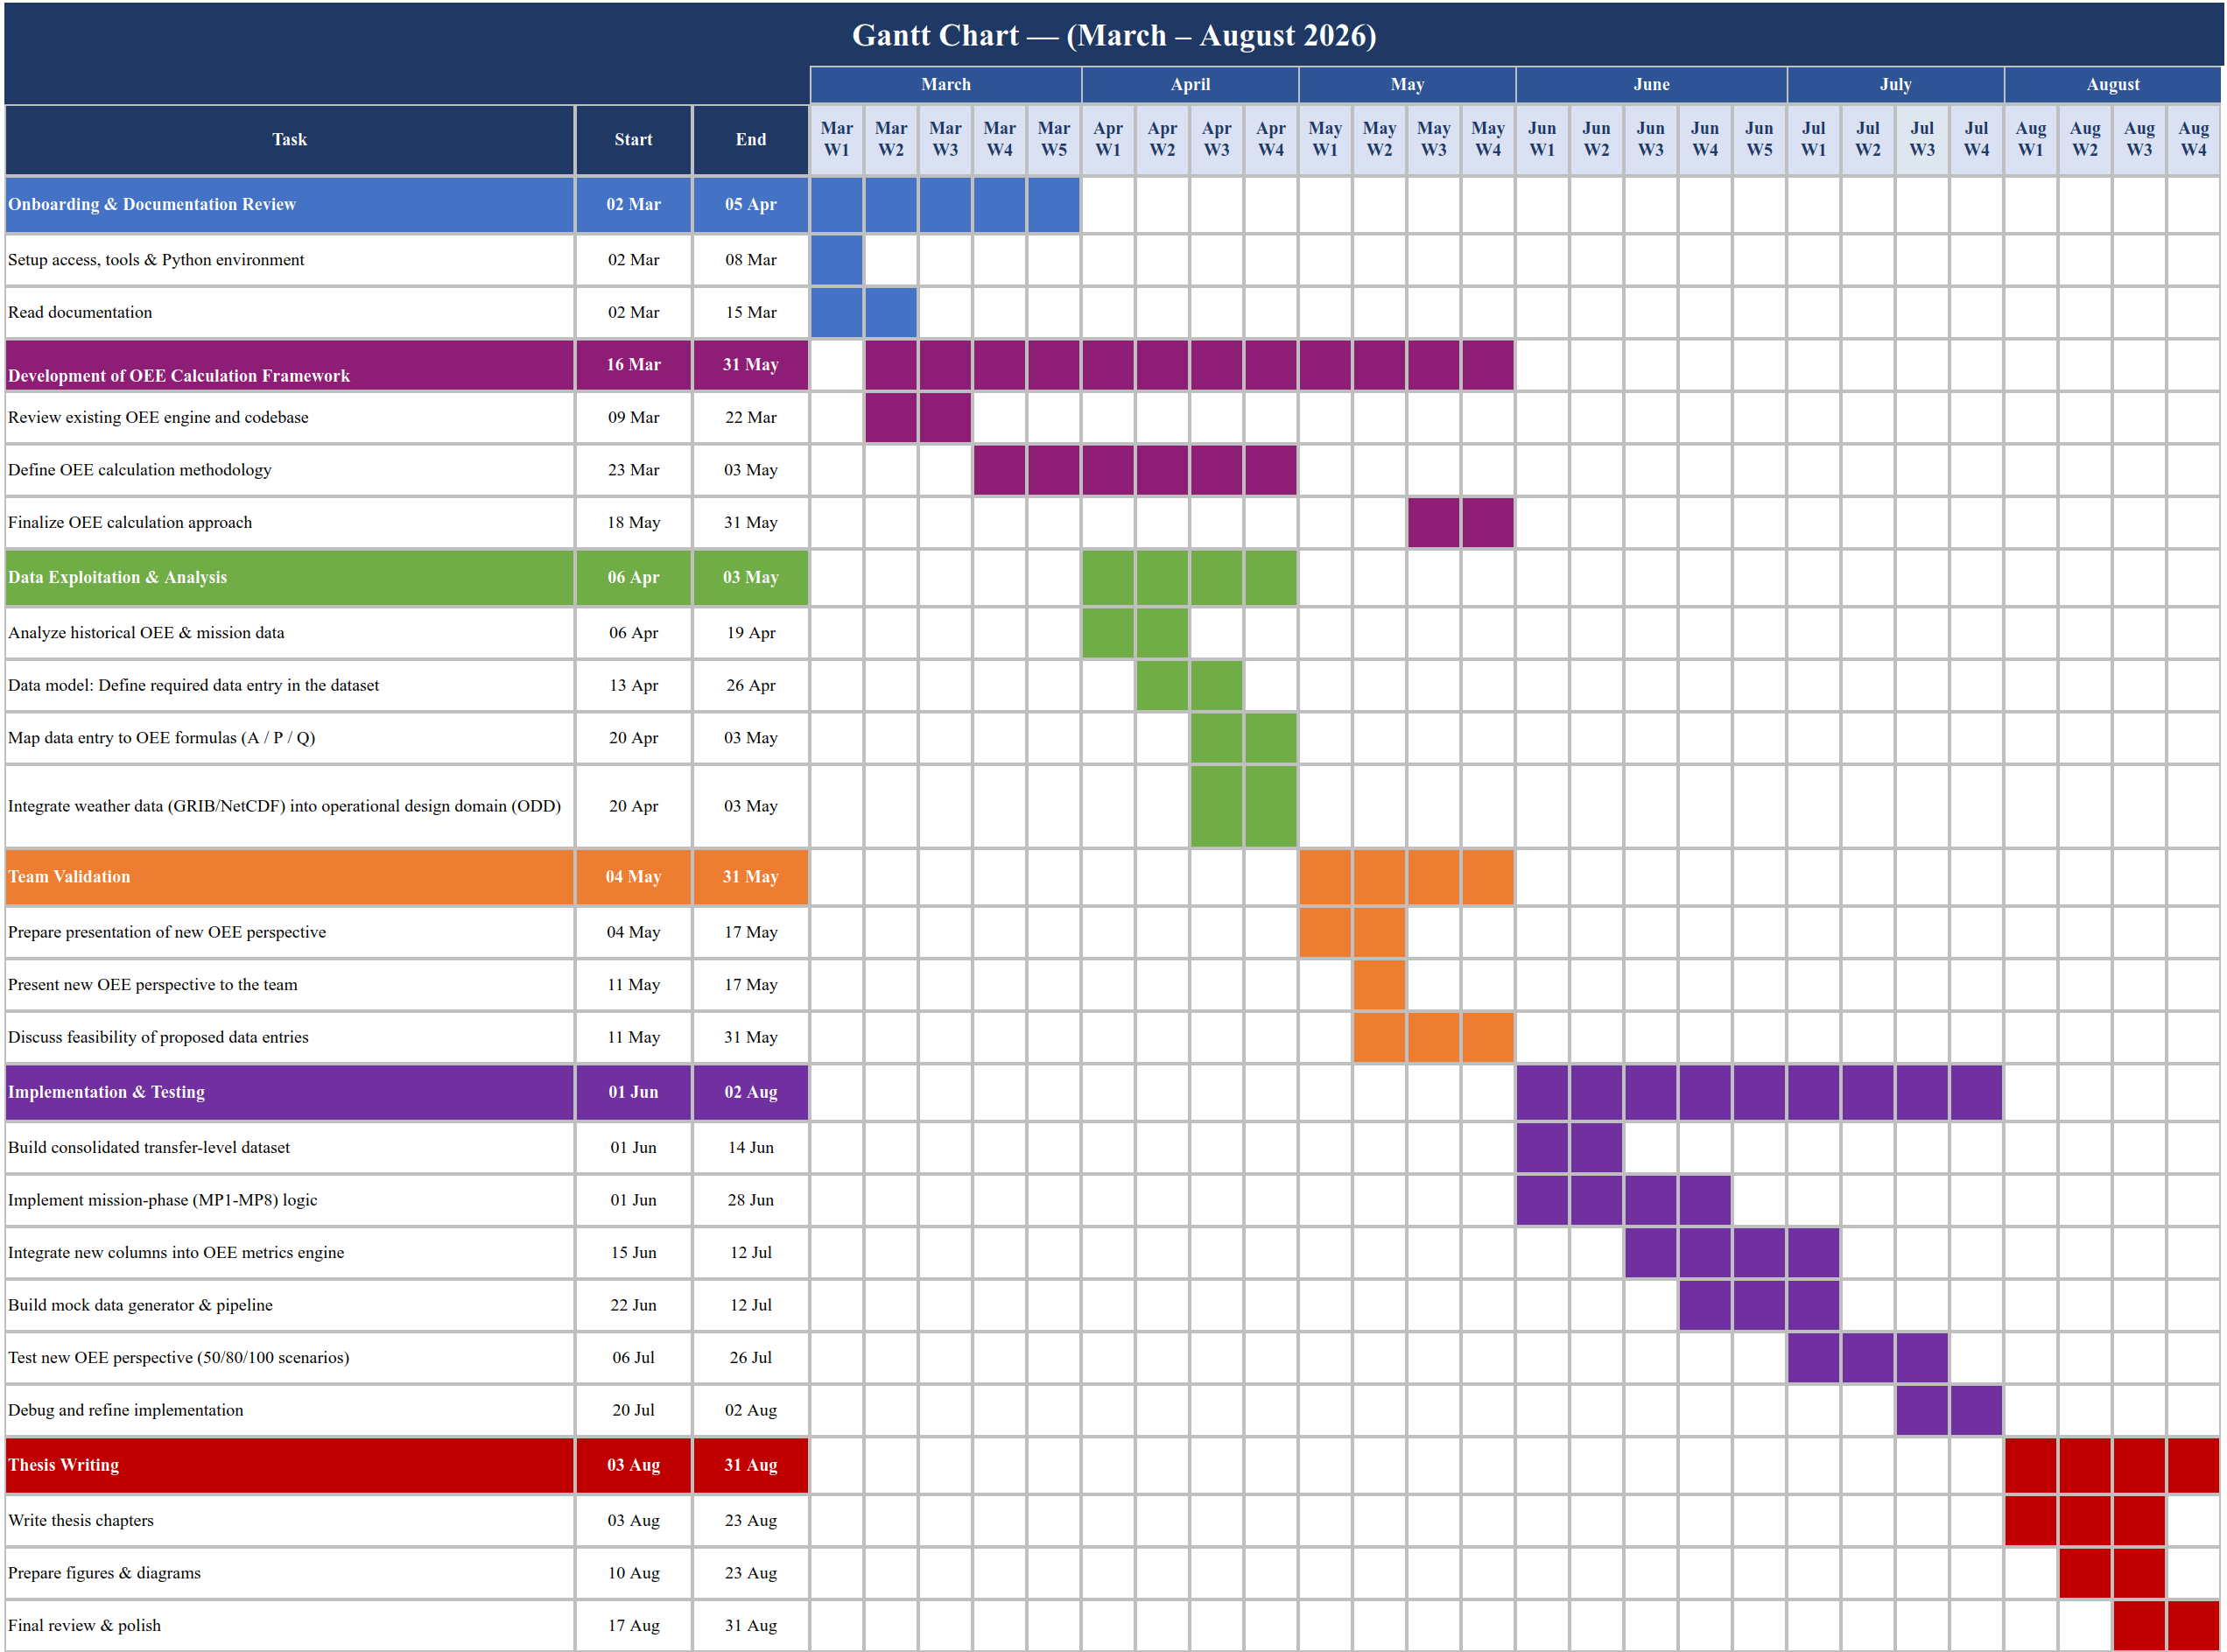
\includegraphics[angle=90, width=1\textwidth]{images/GanttChart.png}
  \caption{Gantt Diagram}
  \label{fig:gantt}
\end{figure}

\section{Conclusion}

This chapter established the industrial and theoretical foundations of the work. It presented TII KAMAG, the autonomous yard-logistics system, its operating environment, system actors, transfer workflow, mission hierarchy, architecture, and data sources. It also showed that operational effectiveness depends on technical performance, mission variability, human supervision, traffic, and environmental conditions.

The review of \gls{oee} showed that Availability, Performance, and Quality provide a useful structure for measuring industrial effectiveness. However, classical \gls{oee} was developed for stable manufacturing systems with fixed cycle times. Autonomous yard vehicles operate under variable conditions and generate specific events, such as interventions, disengagements, autonomy limitations, and ODD-related exclusions. Existing autonomous-vehicle \gls{kpi}s, reliability metrics, and capability indices provide valuable information, but they do not combine these aspects into one integrated measure.

These findings define the research gap addressed by this work. \textbf{An adapted \gls{oee} framework is required for autonomous yard logistics}. The framework must account for variable mission durations, autonomy-specific losses, supervision requirements, and ODD-related constraints. The following chapter presents its measurement unit, time hierarchy, adapted \gls{oee} factors, loss classification, \gls{odd} treatment, and complementary indicators.

\cleardoublepage


  

\chapter{Study of the Existing System}

\section*{Introduction}

This chapter presents a detailed analysis of the existing weather monitoring system in place at Unisphere. The purpose is to understand its current architecture, evaluate its components, and identify its operational strengths and weaknesses. The system includes a combination of sensor hardware, embedded devices, and cloud-based services that together form a pipeline for real-time environmental data acquisition and delivery. Through this analysis, we aim to assess the efficiency, reliability, and scalability of the existing setup, and to highlight opportunities for improvement. These insights provide a foundation for the design and integration of new components in subsequent chapters.

\section{System Description}

\subsection{System Overview}


The system under study is a weather station designed to collect and transmit real-time meteorological data. It integrates a Vaisala WXT536 sensor, which measures parameters such as wind speed, temperature, humidity, pressure, and precipitation. The sensor communicates with a \gls{revpi} industrial controller over an \gls{rs485} interface. On the \gls{revpi}, the data is parsed and formatted before being sent to the cloud via \gls{aws} AppSync. The primary goal of this system is to support Unisphere’s mission of enabling safe and optimized flight operations through the NOVA platform. By providing high-quality, real-time weather data, the system enhances situational awareness, supports trajectory planning, and contributes to safety assessments.\\
Figure~\ref{fig:system-overview-hybrid} illustrates the overall structure of the weather station. 
It highlights the main data flow from the sensors to the RevPi, the cloud, and finally NOVA, while also showing the supporting infrastructure such as power supply, surge protection, and remote management tools.

\begin{figure}[H]
\centering
\begin{adjustbox}{width=\textwidth}
\begin{tikzpicture}[
  font=\small,
  node distance=10mm and 12mm,
  comp/.style={draw, rounded corners=2pt, inner sep=3mm, align=center},
  group/.style={draw, rounded corners=2pt, inner sep=3mm, align=center, fill=black!3},
  flow/.style={-{Latex}, thick},
  mgmt/.style={densely dotted, -{Latex}, thick},
  power/.style={dashed, -{Latex}, thick}
]

% Sensors group
\node[group, label={[label]above:Sensors}] (sensors) 
{\parbox{4.3cm}{\centering \textnormal{\textbf{Vaisala WXT536}\\[-2pt] (ASCII over RS-485, 19200)}}};

% RevPi
\node[comp, right=28mm of sensors] (revpi) 
{\parbox{4cm}{\centering \textnormal{\textbf{RevPi Connect+}\\Raspberry Pi OS (Bookworm)\\Python 3.11 + systemd}}};


% Cloud group
\node[group, right=22mm of revpi, label={[label]above:AWS Cloud}] (cloud) 
{\parbox{5.4cm}{\centering \textnormal{
\textbf{AppSync} (GraphQL API)\\
\textbf{Cognito} (Auth)\\
\textbf{DynamoDB} (Realtime store)\\
\textbf{Lambda / EventBridge / CloudWatch}
}}};

% User apps
\node[comp, right=22mm of cloud] (apps) 
{\parbox{3cm}{\centering \textnormal{\textbf{NOVA}\\Dashboards / APIs}}};

% Power + surge
\node[comp, below=20mm of sensors] (surge) 
{\parbox{3cm}{\centering \textnormal{Vaisala\\Surge Protector}}};
\node[comp, below=18mm of revpi] (psu) 
{\parbox{3.5cm}{\centering \textnormal{DRL-24V480W1EN\\24\,V DC Power Supply}}};

% Management block
\node[comp, above=18mm of revpi] (mgmt) 
{\parbox{3cm}{\centering \textnormal{Qbee / SSH\\(Remote Mgmt)}}};

% Connections
\draw[flow] (sensors.east) -- node[above, sloped]{RS-485 (ASCII)} (revpi.west);
\draw[flow] (revpi) -- node[above, sloped]{Ethernet/4G} (cloud);
\draw[flow] (cloud) -- (apps);

\draw[power] (psu.north) -- ++(0,7mm) -| (revpi.south);
\draw[power] (psu.west) -- ++(-18mm,0) |- (surge.east);
\draw[power] (surge.north) -- ++(0,7mm) -| (sensors.south);

\draw[mgmt] (mgmt) -- (revpi);

% Legend
\node[align=left, anchor=north west] at ($(psu.south west)+(-2mm,-13mm)$) {
\begin{tikzpicture}[x=1cm,y=0.5cm]
\draw[flow] (0,0) -- +(0.8,0) node[right, black]{Data flow};
\draw[power] (0,-0.8) -- +(0.8,0) node[right, black]{Power};
\draw[mgmt] (0,-1.6) -- +(0.8,0) node[right, black]{Remote management};
\end{tikzpicture}
};

\end{tikzpicture}
\end{adjustbox}
\caption{System overview: functional data flow with supporting infrastructure (power, surge, remote management).}
\label{fig:system-overview-hybrid}
\end{figure}




\subsection{Hardware Architecture}

The initial deployment of the weather station system includes a compact yet robust set of components designed for industrial reliability and field deployment. The setup is composed of the Revolution Pi Connect+ as the central processing unit, connected via dedicated RS-485 interfaces to the Vaisala WXT536 and \gls{pwd12} sensors. The \gls{revpi} also connects to the 24 V DC power supply that feeds both sensors. The network connection (Ethernet/4G) provides the link to the cloud backend. This arrangement ensures that each sensor operates on an independent communication bus with the correct baud rate, reducing cross-talk and improving reliability in remote deployments.



%\begin{figure}[H]
%  \centering
%  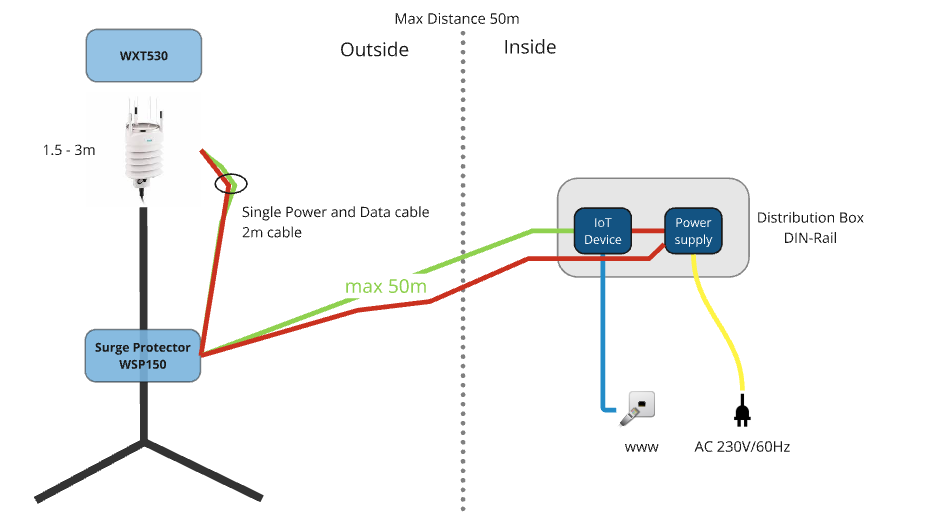
\includegraphics[width=0.8\textwidth]{images/HARD.png}
%  \caption{Actual System Architecture}
%  \label{fig:hard}
%\end{figure}



\subsubsection*{Main Hardware Components}
\begin{itemize}
    \item \textbf{Vaisala WXT536:} Multi-parameter weather sensor measuring wind, temperature, humidity, pressure, and precipitation.
    \item \textbf{\gls{revpi} Connect+:} Industrial Raspberry Pi-based controller responsible for data parsing and cloud integration.
    \item \textbf{DRL-24V480W1EN:} \gls{din}-rail industrial power supply delivering stable 24\,V\,DC.
    \item \textbf{Vaisala Surge Protector:} Protects the system against lightning-induced voltage spikes.
    \item \textbf{Heavy-duty Mast:} A freestanding lamp stand used to mount the sensor outdoors.
    \item \textbf{Industrial Ethernet Switch (IDS-105FE):} Provides network connectivity between \gls{revpi} and backend services.
    \item \textbf{Cables and Connectors:} Including an 8-pin M12 cable for power and \gls{rs485} communication.
\end{itemize}



\subsubsection*{Power and Communication}
\begin{itemize}
    \item \textbf{Power Input:} 230\,V\,AC supplied to the DRL power supply.
    \item \textbf{Sensor Power:} 24\,V\,DC provided to the WXT536.
    \item \textbf{Communication Interface:} RS-485 using an 8-pin M12 connector (differential A/B lines).
    \item \textbf{\gls{revpi} Serial Port:} Typically \texttt{/dev/ttyAMA5} or \texttt{/dev/ttyAMA4} depending on wiring configuration.
\end{itemize}

\subsubsection*{Installation and Protection}
\begin{itemize}
    \item \textbf{Mounting:} Pole-mounted setup suitable for testing and outdoor deployments.
    \item \textbf{Grounding:} Properly grounded and protected against electrical surges.
    \item \textbf{Enclosure:} Components placed in a sealed electrical box for weather protection.
\end{itemize}



\subsection{Communication Interfaces}

The system relies on a combination of serial and cloud-based communication interfaces to ensure seamless data flow from sensor to cloud platform.

\begin{itemize}
  \item \textbf{Sensor-to-Controller Communication:}  
  The Vaisala WXT536 sensor communicates with the \gls{revpi} using the \textbf{\gls{ascii} protocol} over an \textbf{\gls{rs485}} physical interface. The communication is configured at a \textbf{baud rate of 19200}. A twisted pair configuration is used for the \gls{rs485} line, and an M12 8-pin connector is employed to connect the sensor to the electric box.

  \item \textbf{Data Handling on the \gls{revpi}:}  
  Upon reception, the sensor messages are verified using a \textbf{\gls{crc} checksum} to ensure data integrity. Once validated, the data is parsed and formatted into a readable structure for further use and transmission.

  \item \textbf{Controller-to-Cloud Communication:}  
  The parsed weather data is transmitted in real-time to the cloud using \textbf{\gls{aws} AppSync}, a GraphQL-based service that supports low-latency communication. Data is not batched, but pushed directly upon reception and validation.

  \item \textbf{Remote Access and Monitoring:}  
  Remote access to the \gls{revpi} is achieved through \textbf{\gls{ssh}} using its \gls{ip} address when connected to the office Ethernet network. Additionally, \textbf{Qbee} is used as a remote monitoring and management platform, allowing secure access and deployment from external locations.

  \item \textbf{Surge Protection:}  
  Although surge protection is primarily applied to the power lines, the communication setup benefits indirectly from the protected environment within the electric enclosure, reducing the risk of hardware damage.
\end{itemize}


\subsection{Software Stack and Cloud Services}

The system is built around a lightweight but robust software stack running on an industrial-grade controller, with full integration into \gls{aws} cloud services. Figure \ref{fig:cloudflow} presents a high-level view of the software and cloud architecture, illustrating the flow of data from sensor acquisition to real-time cloud transmission and backend interaction. The software and cloud components are structured as follows:


\begin{itemize}
  \item \textbf{Programming Language:}  
  The entire application logic is implemented in \textbf{Python}, which provides a balance between rapid development and system-level hardware communication capabilities.

  \item \textbf{Runtime Environment:}  
  The \gls{revpi} Connect+ controller runs \textbf{Raspbian GNU/Linux 12 (Bookworm)}, a Debian-based operating system. The Python application is executed within a \textbf{\gls{venv}} to ensure package isolation, and is deployed as a \textbf{systemd service} to guarantee automatic startup and resilience after reboots.

  \item \textbf{Data Handling and Parsing:}  
  Sensor data is received via the \gls{rs485} interface and is subject to a \textbf{\gls{crc} checksum validation}. Once validated, the \gls{ascii}-formatted message is parsed into a structured format suitable for cloud transmission. 

  \item \textbf{Cloud Integration:}  
  Real-time weather data is transmitted to the cloud via \textbf{\gls{aws} AppSync}, using a GraphQL \gls{api} endpoint. This allows efficient and structured interaction with backend services while enabling real-time data availability.

  \item \textbf{Authentication and Security:}  
  Authentication is managed via \textbf{\gls{aws} Cognito}, and access to the AppSync endpoint is secured using an \textbf{\gls{api} key}, stored in environment variables to prevent hardcoding credentials within the source code.
  
  \item \textbf{Supporting AWS Services:}  
  In addition to AppSync and Cognito, other AWS services are integrated in the backend to support system monitoring and data processing. These include \textbf{DynamoDB} for storing incoming weather records, \textbf{CloudWatch} for runtime monitoring and logging, and \textbf{EventBridge}, which is used internally for identifying inactive sensors and automating alerting and historical weather data preprocessing.


  \item \textbf{Deployment and Maintenance:}  
  For \gls{vcs}, we use \textbf{Git}. Updates are pushed to the \gls{revpi} either via local access or remotely using \textbf{Qbee}, a device management platform that supports remote monitoring and secure \gls{ssh} access.
\end{itemize}


\begin{figure}[H]
    \centering
    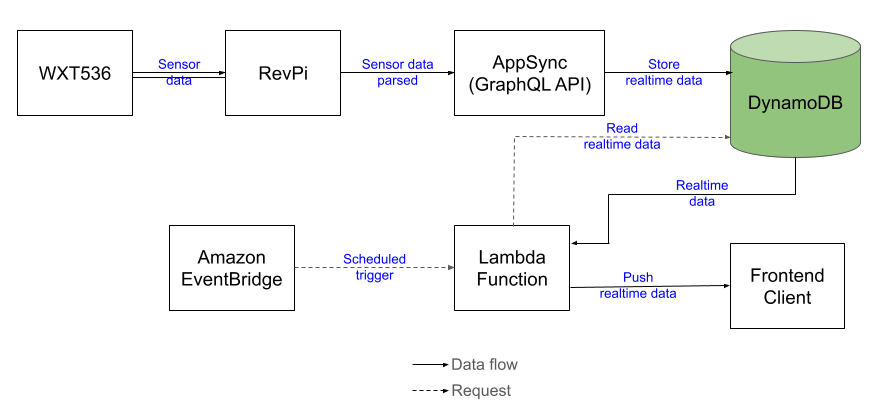
\includegraphics[width=\textwidth]{images/cloud flow.png}
    \caption{Data Flow Architecture}
    \label{fig:cloudflow}
\end{figure}

\section{System Evaluation}

\subsection{System Strengths}

The weather station system designed by Unisphere exhibits several strengths that contribute to its operational effectiveness, maintainability, and integration potential.

\subsubsection{Robustness and Reliability}

The existing system, prior to the integration of the new visibility sensor, was architected for operational stability and reliability in long-term deployments. The software runs as a \texttt{systemd} service on the \gls{revpi}, which ensures automatic restarts in case of unexpected shutdowns or power failures. In addition, error handling mechanisms are implemented through \gls{crc} checksum validation and structured message parsing. These features contribute to reducing the likelihood of system crashes and ensuring consistent data availability over time. 


\subsubsection{Simplicity and Modularity}

The system architecture follows a modular design that separates sensor communication, data parsing, and cloud transmission into distinct functional layers. This separation allows for clear interfaces between components and simplifies both debugging and future extensions. For instance, the code responsible for parsing data from the sensor is encapsulated in independent modules, which can be reused or adapted for other sensors. The availability of an unused RS-485 port on the \gls{revpi} further simplified the physical integration of the new Vaisala \gls{pwd12} sensor, requiring minimal disruption to the existing setup. Overall, the modular structure enables scalable development without requiring a complete system overhaul.


\subsubsection{Cloud Integration}

The system benefits from seamless integration with \textbf{\gls{aws}} cloud services, particularly through the use of AppSync for real-time data streaming. This integration ensures immediate availability of weather data for backend services and frontend applications. AppSync enables efficient communication using GraphQL, which allows clients to fetch precisely the data they need, minimizing payload size and reducing response latency. The use of scalable cloud services also facilitates future extensions, such as long-term storage, alerting, and analytics.

\subsection{Limitations and Opportunities for Improvement}

While the weather station system demonstrates robustness and modularity, certain technical limitations were identified during the integration work. These limitations represent opportunities for further refinement in future system iterations.

\subsubsection{Lack of Visibility Measurement}

The existing weather station provides valuable meteorological data such as wind, precipitation, temperature, humidity, and pressure. However, it does not include visibility measurements, which are critical for aviation-related applications. Visibility data directly supports decision-making for flight safety, landing operations, and trajectory planning. The absence of this parameter reduces the system’s ability to deliver a comprehensive picture of atmospheric conditions.



\subsubsection{Protocol and Communication Constraints}

The system relies on the \gls{rs485} interface for communication with the weather sensors. While \gls{rs485} is reliable for industrial serial communication, it requires all connected devices to operate at the same baud rate. This constraint limits the possibility of using multiple sensors with different serial configurations on the same line.  
Moreover, the current setup uses the \gls{ascii} protocol, which, although simple, is less efficient in terms of message size and validation. Alternative protocols like Modbus \gls{rtu} may offer improvements in reliability and bandwidth usage. A comparative overview is shown in Table~\ref{tab:protocol-comparison}.

\begin{table}[!ht]
\renewcommand{\arraystretch}{1.5}
\centering
\caption{Comparison between \gls{ascii} and Modbus \gls{rtu} protocols}
\label{tab:protocol-comparison}
\begin{tabular}{|c|c|c|}
\hline
\textbf{Aspect} & \textbf{\gls{ascii} Protocol} & \textbf{Modbus \gls{rtu} Protocol} \\
\hline
Message Format & Human-readable characters & Binary format \\
\hline
Bandwidth Efficiency & Lower (larger messages) & Higher (compact messages) \\
\hline
Error Detection & Typically \gls{crc} or checksum & \gls{crc} integrated \\
\hline
Ease of Debugging & Easier (text-based) & Harder (binary) \\
\hline
Message Size & Larger due to encoding & Smaller and more efficient \\
\hline
\end{tabular}
\end{table}

\subsubsection{Lack of Offline Resilience}

The original version of the weather station system was designed with the assumption of continuous internet connectivity. However, operational experience with different customer deployments revealed that connectivity disruptions can occur — for example, due to network outages or infrastructure work within the client’s network environment. In such cases, the system is unable to transmit weather data to the cloud, leading to permanent data loss during the offline period.

This limitation affects the completeness and continuity of the dataset, which are essential for use cases such as real-time monitoring, retrospective analysis, and flight simulation validation. Enhancing the system to support offline buffering and delayed transmission is therefore a critical area for future improvement.

\subsubsection{Data Handling and Storage Gaps}

The current system uses an \textbf{\gls{aws} DynamoDB} table to store incoming weather records, each of which is assigned a \textbf{\gls{ttl}} attribute of 48 hours. This design ensures that outdated entries are automatically deleted, allowing the system to maintain a lightweight and cost-efficient database while supporting real-time weather monitoring.

Although short-term retention is sufficient for most operational needs, certain use cases — such as long-term analysis, retrospective evaluations, or training of predictive models — require permanent access to historical weather data. Figure \ref{fig:cloud improved} illustrates an architectural extension that incorporates a dedicated cloud storage layer. This improvement allows the system to maintain its real-time performance while enabling historical data archiving in a scalable and structured manner.

\begin{figure}[H]
  \centering
  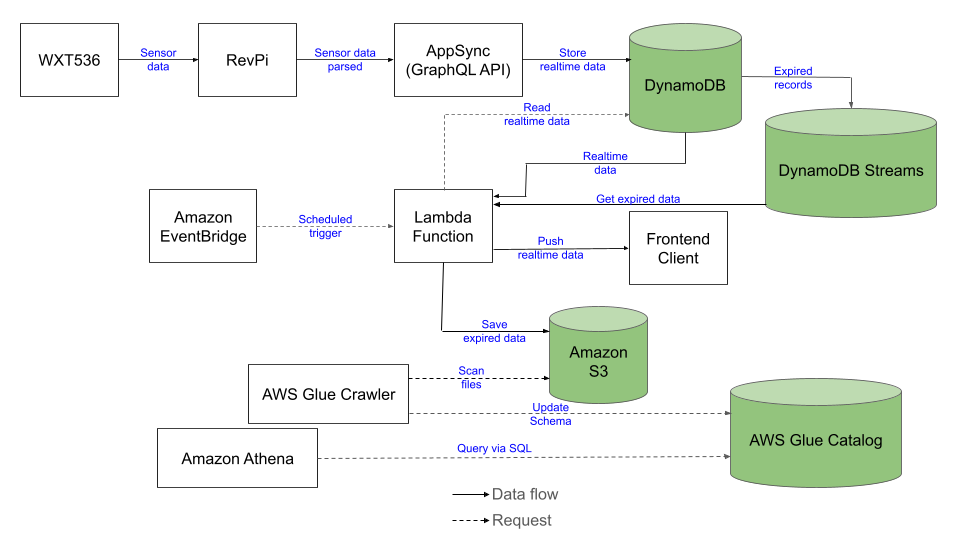
\includegraphics[ width=\textwidth]{images/cloud improved.png}
  \caption{Proposed improvement to cloud architecture with persistent data storage}
  \label{fig:cloud improved}
\end{figure}



\subsubsection{Scope of This Work}

The analysis above highlights three main limitations of the existing weather station system: protocol and communication constraints, gaps in data storage, and lack of offline resilience.  
However, not all of these gaps fall within the scope of the present work.

In this thesis, two aspects are addressed directly:
\begin{itemize}
    \item \textbf{Integration of a new visibility measurement:} The Vaisala PWD12 sensor is added to complement the WXT536 and extend the system’s measurement capabilities.
    \item \textbf{Enhancing offline resilience:} A local buffering mechanism based on SQLite is implemented to prevent data loss during temporary connectivity outages.
\end{itemize}

The following limitations are acknowledged but not solved within this work:
\begin{itemize}
    \item \textbf{Protocol and communication constraints:} A theoretical improvement could be achieved by adopting Modbus RTU instead of ASCII, allowing more efficient message formats and flexible baud rate handling. This would require substantial changes in both firmware configuration and software parsing, and is therefore considered out of scope for this thesis.
    \item \textbf{Data storage gaps:} A potential solution is to introduce a cloud-based persistent storage layer (e.g. Amazon S3 or a time-series database) to complement DynamoDB’s short-term retention. This would enable historical analysis and model training, but lies outside the immediate objectives of this work.
\end{itemize}

This scoping ensures that the thesis remains focused on sensor integration and operational robustness, while still acknowledging other improvement paths for the system.



\section*{Conclusion}
With a clear understanding of the existing weather station system, including its architecture, strengths, and limitations, the focus now shifts to the detailed study of the new visibility sensor selected for integration: the Vaisala \gls{pwd12}. This chapter provided a comprehensive examination of the sensor’s internal design, operating principles, and technical specifications, as well as its relevance to the system’s operational objectives. This foundational understanding is essential to ensure effective hardware integration, data parsing, and long-term reliability within the broader weather monitoring platform.



\cleardoublepage



\chapter{Study of the PWD12 Sensor}
\label{chap:pwd12-study}

\section*{Introduction}

This chapter focuses on the Vaisala \gls{pwd12} visibility sensor, shown in figure~\ref{fig:pwd}, a key component to be integrated into the weather monitoring system. The study covers its functionality, measurement principles, supported features, and communication capabilities. Special attention is given to the configuration process, the command interface, and how the sensor behaves in standalone testing scenarios. Understanding the \gls{pwd12}’s capabilities and requirements is essential before proceeding with its integration into the broader system. This chapter establishes the technical basis for ensuring reliable operation and effective data acquisition. Unless otherwise specified, all technical details in this chapter are based on the Vaisala PWD22/52 User’s Guide \cite{vaisala2015pwd}.

\begin{figure}[H]
  \centering
  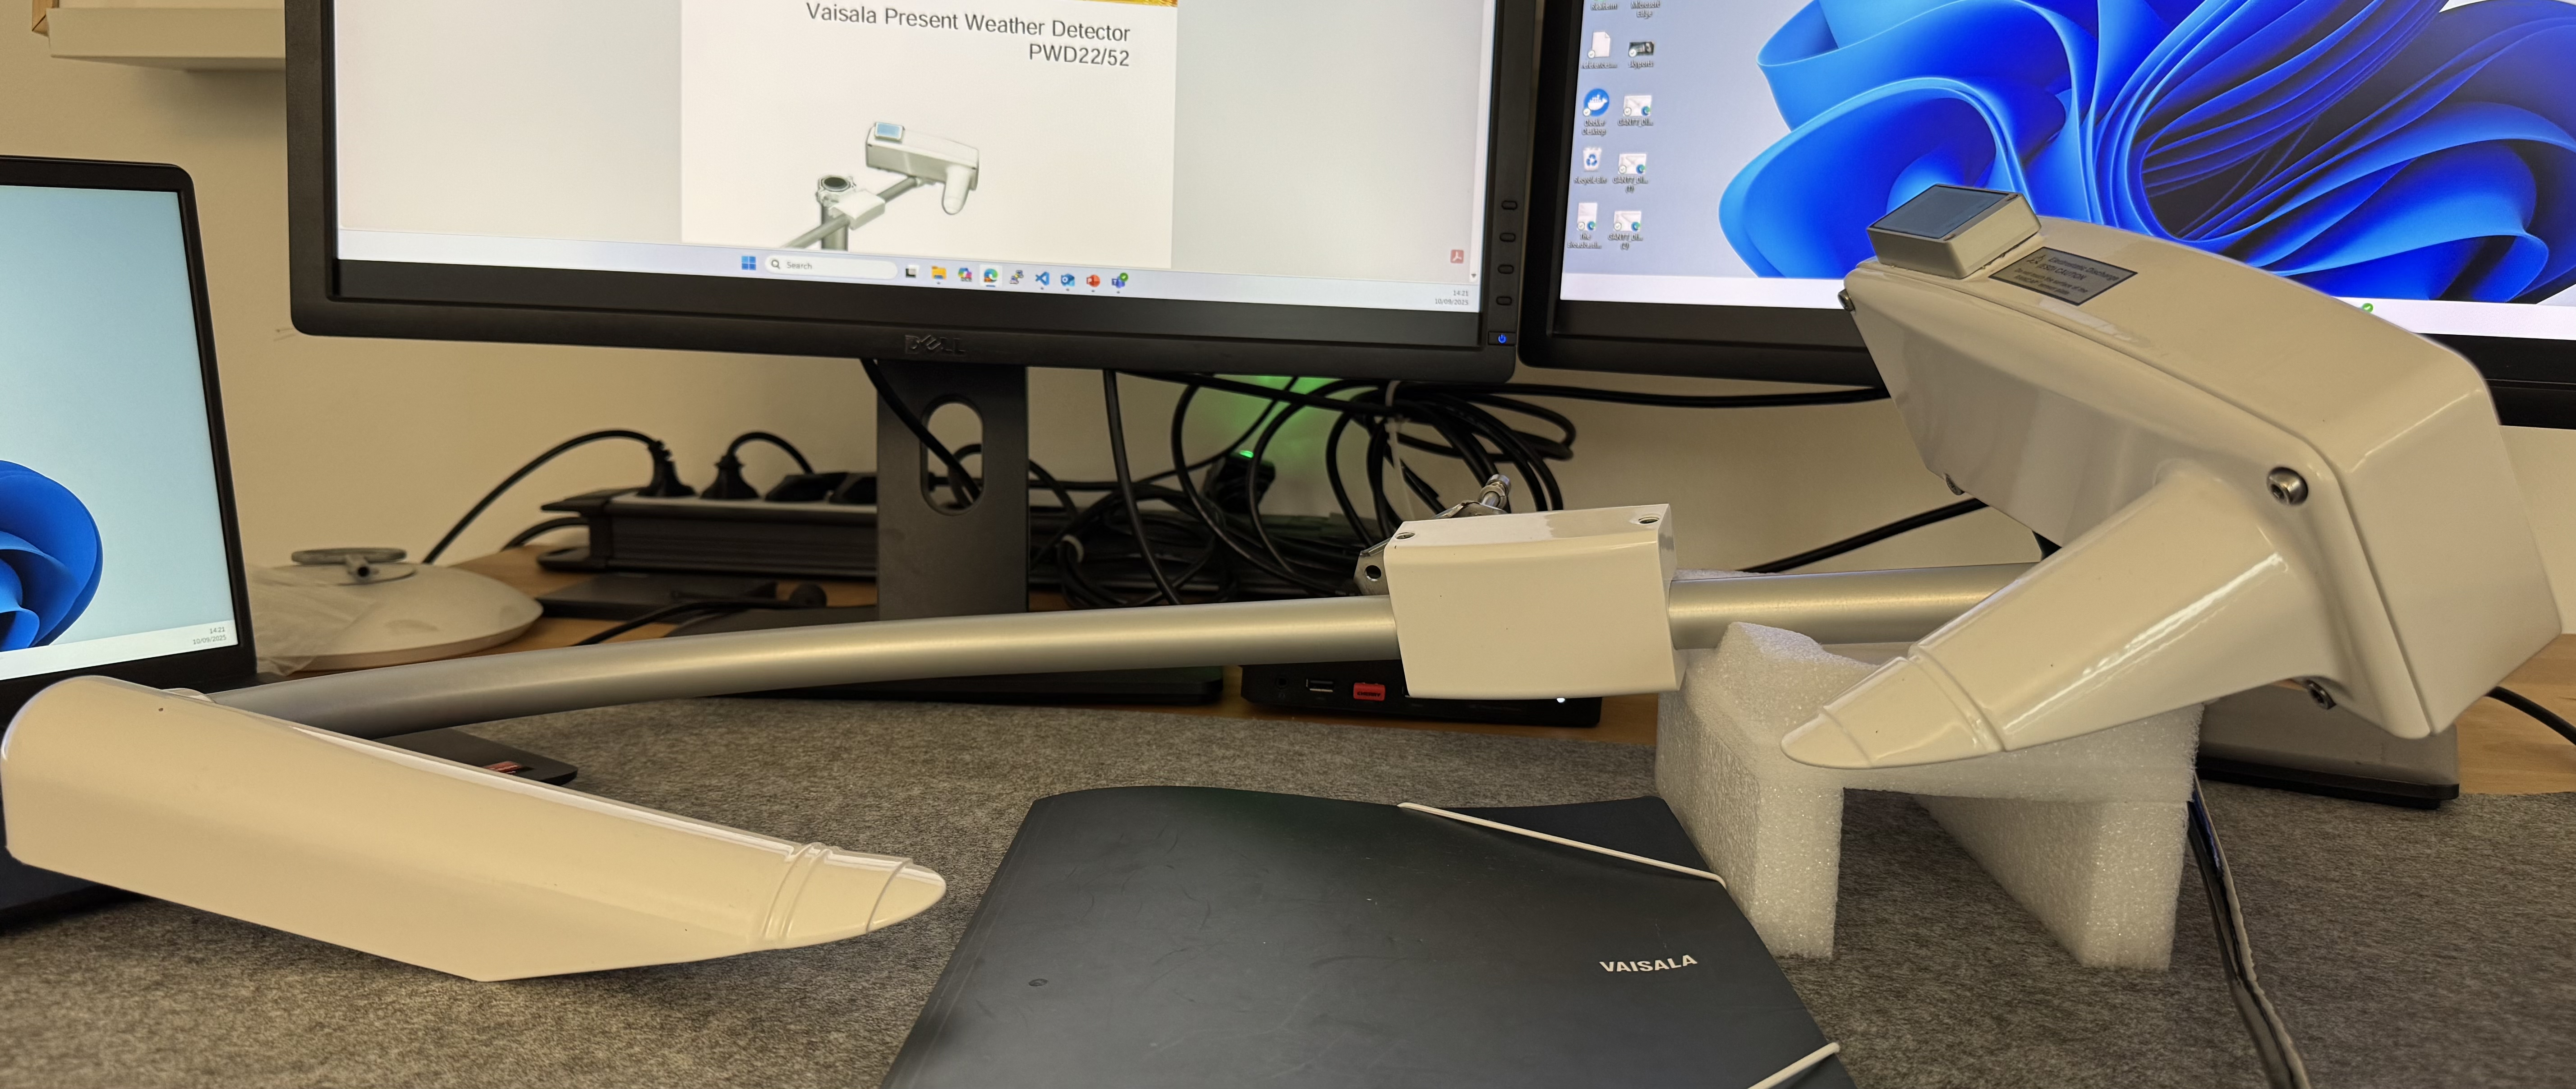
\includegraphics[width=1\textwidth]{images/Vaisala_PWD12.jpg}
  \caption{Vaisala Present Weather Detector PWD12}
  \label{fig:pwd}
\end{figure}

\section{Sensor Context and Operational Role}
\label{sec:pwd_context}

\subsection{Purpose of Integrating the PWD12}

The decision to integrate the \textbf{Vaisala \gls{pwd12}} visibility sensor into the weather station was largely influenced by Unisphere's prior experience with Vaisala hardware and the reliability of their certified instruments. Vaisala's long-standing reputation in meteorological sensing, combined with the sensor's compliance with aviation and meteorological standards, made it a trustworthy addition to the system. Although the decision was made before the start of the internship, the integration aligned well with the company's infrastructure and quality expectations.

\subsection{Role in the Weather Station}

The \gls{pwd12} extends the capabilities of the existing weather station by adding \textbf{visibility measurement}, a parameter that was not captured by the previously installed WXT536 sensor. This enhancement was essential for supporting operational environments such as vertiports, where visibility conditions directly impact the feasibility of air taxi operations.


\subsection{Relevance to UAS Operations and the NOVA Platform}

Visibility data plays a critical role in \textbf{\gls{uas}} operations, particularly under \textbf{\gls{vfr}} and for applications like \textbf{\gls{uam}}. In such contexts, poor visibility can ground flights or require re-routing, making accurate and localized measurement a key enabler for operational decision-making.

Within the NOVA platform, visibility readings contribute to weather-aware flight planning, real-time monitoring, and post-operation analysis. The integration of the \gls{pwd12} is especially relevant for advanced vertiport deployments, such as the one near \gls{dxb}, where air taxi services are planned. In these environments, visibility is not just a regulatory requirement but a critical factor in ensuring safety and operational continuity.



\section{Internal Architecture and Hardware Components}

The Vaisala \gls{pwd12} sensor is a sophisticated device designed to deliver precise visibility and present weather measurements in outdoor environments. This section explores its internal structure and the physical components that contribute to its functionality.

\subsection{Optical Measurement System}

At the core of the visibility measurement functionality is the \gls{pwd12}’s \textbf{forward-scatter optical system} \cite{vaisala2015pwd}. It consists of an infrared light source and a photodetector arranged at a 42° angle relative to each other. When light emitted by the source encounters airborne particles like fog or rain, some of the light is scattered and captured by the receiver. The intensity of this scattered light is used to calculate the \textbf{\gls{mor}}.

This arrangement allows for a compact design with minimal maintenance requirements, as it eliminates the need for moving parts. The measurement volume is carefully defined to avoid contamination from precipitation that may pass through but not reflect light effectively.

As shown in Figure \ref{fig:optic}, the layout of the optical components ensures that only forward-scattered light is measured, minimizing noise from ambient light and non-relevant angles.

\begin{figure}[H]
  \centering
  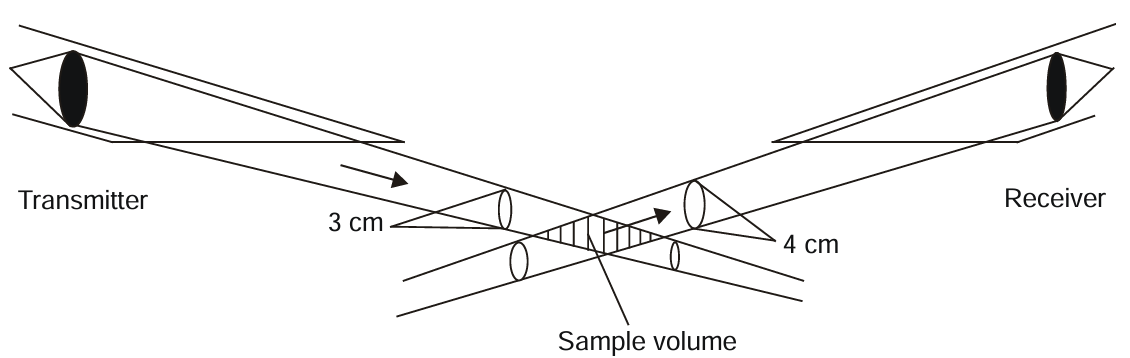
\includegraphics[width=0.9\textwidth]{images/optic.png}
  \caption{\gls{pwd12} Optical System Layout\cite{vaisala2015pwd}}
  \label{fig:optic}
\end{figure}

\subsection{RAINCAP Precipitation Sensor}

In parallel with visibility measurements, the \gls{pwd12} features a \textbf{RAINCAP} sensor\cite{vaisala2015pwd} mounted on the top of the enclosure. This is a solid-state capacitive sensor that detects precipitation through mechanical vibrations caused by raindrops or snowflakes hitting its surface. The internal signal processing algorithm analyzes the impact pattern and frequency to differentiate between precipitation types like drizzle, rain, snow, and sleet.

This mechanism allows for fast and reliable precipitation detection without requiring any moving parts, enhancing durability in the field. The design and principle of operation are illustrated in Figure \ref{fig:raincap}.

\begin{figure}[H]
  \centering
  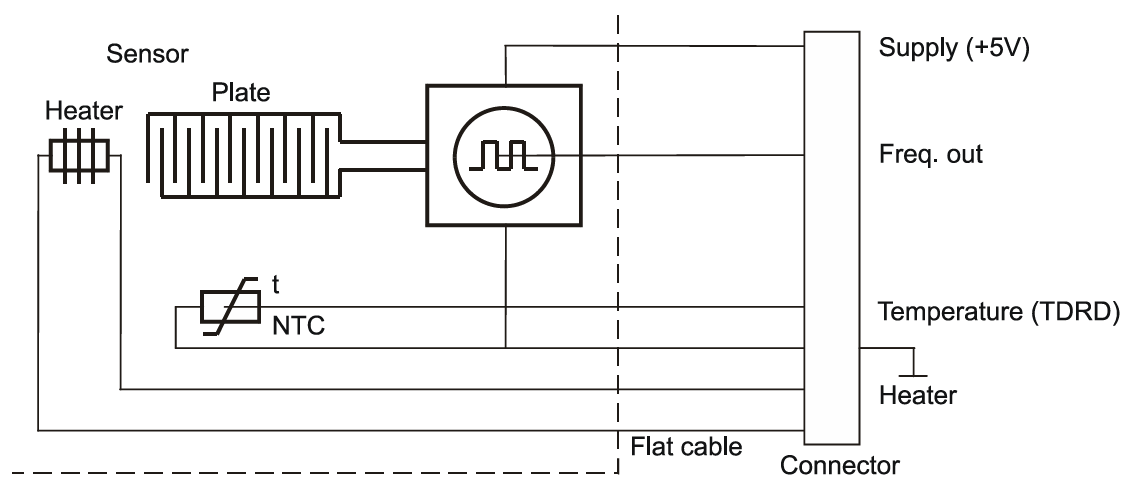
\includegraphics[width=0.9\textwidth]{images/raincap.png}
  \caption{RAINCAP Block Diagram\cite{vaisala2015pwd}}
  \label{fig:raincap}
\end{figure}

\subsection{Anti-Icing and Heating Mechanisms}

To ensure uninterrupted performance in cold and icy conditions, the \gls{pwd12} is equipped with \textbf{automatic heaters}\cite{vaisala2015pwd} located in three zones: the optical head, the RAINCAP sensor, and the main enclosure. These heaters are activated based on environmental conditions and internal temperature readings to prevent snow or ice buildup on sensitive areas.

The heater outputs can be controlled remotely via digital I/O lines or allowed to operate autonomously. The heater configuration helps maintain consistent measurement accuracy regardless of the surrounding weather.

\subsection{Signal Processing Unit and Embedded Controller}

All sensor outputs are processed by an embedded microcontroller inside the \gls{pwd12}. This unit is responsible for:
\begin{itemize}
    \item Converting raw analog signals into digital measurements,
    \item Filtering and applying classification algorithms,
    \item Generating weather codes and output strings,
    \item Managing communication and diagnostic reporting.
\end{itemize}

\subsubsection{Enclosure and Protection}

The Vaisala \gls{pwd12} is housed in a rugged, \textbf{\acrshort{ip66}-rated enclosure}\cite{vaisala2015pwd}, designed for long-term deployment in demanding outdoor environments. The enclosure combines \textbf{anodized aluminum} with \textbf{\acrshort{uv}-resistant polycarbonate} to ensure structural integrity, weather resistance, and longevity.

Key features of the protective design include:

\begin{itemize}
    \item \textbf{Ingress Protection:} The \gls{ip66} rating guarantees that the enclosure is dust-tight and protected against strong water jets from any direction, making it suitable for exposed locations.
    
    \item \textbf{\gls{emc} Shielding:} The internal electronics are shielded to comply with \textbf{\gls{en61326}}, reducing susceptibility to electrical interference from nearby equipment or power lines. This is essential when the sensor is installed near radar, communication antennas, or industrial machinery.
    
    \item \textbf{Grounding and Surge Protection:} A dedicated grounding terminal allows the sensor to be connected to the site’s earthing system. Additionally, the PWD12 includes internal protection components against electrostatic discharge and transient surges on communication and power lines. However, external surge arrestors are recommended for full compliance with installation best practices.
    
    \item \textbf{Environmental Robustness:} The physical form factor minimizes accumulation of snow, debris, or bird droppings on optical and sensing elements. The sloped housing design promotes self-cleaning, reducing maintenance needs.
    
    \item \textbf{Connector Interface:} The cable gland or M12 interface is sealed to prevent moisture ingress while providing mechanical strain relief for the cable.
\end{itemize}

These protection features make the \gls{pwd12} well-suited for aviation and meteorological applications where \textbf{continuous and interference-free operation} is essential.


\section{Technical Specifications}

The Vaisala \gls{pwd12} sensor is designed to provide high-accuracy visibility and present weather measurements. It outputs a variety of environmental parameters relevant for \gls{uas} operations, particularly under \gls{vfr} conditions.

\subsection{Measurable Parameters and Units}

The \gls{pwd12} outputs a rich set of weather data using periodic \gls{ascii} messages\cite{vaisala2015pwd}. The standard configuration includes the following measurements:
\begin{itemize}
    \item \textbf{Visibility}: 1-minute and 10-minute averaged visibility values (in meters).
    \item \textbf{Present Weather Codes}: Instantaneous, 15-minute, and 1-hour weather conditions using both \gls{nws} and \gls{wmo} code standards.
    \item \textbf{Precipitation}: Intensity (mm/h), cumulative precipitation (mm), and snow accumulation (mm).
    \item \textbf{Optional Parameters}: Air temperature (°C) and background luminance (cd/m²) can also be measured when Message 7 is enabled.
\end{itemize}


\subsection{Accuracy, Resolution, and Operating Ranges}

Table \ref{tab:pwd12specs} summarizes key performance parameters for the visibility and precipitation-related measurements\cite{vaisala2025pwd12}.
\begin{table}[H]
\small
\renewcommand{\arraystretch}{1.5}
\setlength{\tabcolsep}{8pt} % Adjust column padding

\centering
\caption{\gls{pwd12} Visibility Sensor Measurement Characteristics (See PWD Datasheet\cite{vaisala2025pwd12})}
\label{tab:pwd12specs}
\begin{tabular}{|p{3cm}|c|c|c|p{3.5cm}|}
    \hline
    \textbf{Parameter} & \textbf{Range} & \textbf{Interval} & \textbf{Uncertainty} & \textbf{Notes} \\
    \hline
    Visibility (1/10 min) & 1--2000 m & 15 s & ±10\% or ±2.5\% & Averaged over 1 and 10 minutes \\
    \hline
    Precipitation Intensity & 0--999.99 mm/h & 15 s & ±2.5\% & Resolution: 0.05 mm \\
    \hline
    Cumulative Precipitation & 0--99.99 mm & 15 s & ±2.5\% & Reset on restart or CLRS command \\
    \hline
    Snow Accumulation & 0--999 mm & 15 s & ±2.5\% & Reset on restart or CLRS command \\
    \hline
    Present Weather Code & 0--99 & 15 s & – & Based on optical and Doppler signals \\
    \hline
\end{tabular}
\end{table}

\subsection{Supported Message Types and Baud Rates}

The sensor is configured to emit \texttt{Message 2}, which contains the present weather status in standard format, and optionally \texttt{Message 7}\cite{vaisala2015pwd} for aviation-specific use. These messages are structured in the \gls{ascii} protocol and transmitted periodically over the \gls{rs485} interface.

Each message includes a \gls{crc} checksum for error detection, and consists of multiple comma-separated fields representing visibility, weather codes, precipitation levels, and optional extensions such as temperature and luminance.


\subsection{Power Requirements and Electrical Characteristics}

The \gls{pwd12} requires separate power inputs for its measurement electronics and its integrated heater system\cite{vaisala2015pwd}:

\begin{itemize}
    \item \textbf{Measurement Electronics:} 12–50\,V\,DC
    \item \textbf{Heaters:} 24\,V\,DC recommended
\end{itemize}

The sensor is designed for outdoor environments and includes built-in features for environmental resilience:
\begin{itemize}
    \item \textbf{Operating Temperature:} -40\textdegree{}C to +60\textdegree{}C
    \item \textbf{Ingress Protection:} \gls{ip66}-rated enclosure
    \item \textbf{\gls{emc} Protection:} The electronics comply with EN61326-1 and EN55011 Class B emission limits.
    \item \textbf{Mounting:} Vertical mounting with proper optical alignment (receiver facing north in the northern hemisphere).
\end{itemize}

\section{Installation and Environment Requirements}

Proper installation is crucial to ensure the long-term reliability, accuracy, and durability of the \gls{pwd12} sensor. Vaisala provides clear guidelines to mitigate environmental interference and support optimal sensor performance.

\subsection{Site Selection Guidelines}

The sensor must be installed in an open area with unobstructed airflow and visibility. According to Vaisala's recommendations\cite{vaisala2015pwd}:

\begin{itemize}
    \item A \textbf{minimum horizontal clearance of 100\,m} should be maintained from large objects such as buildings, trees, or towers.
    \item The sensor should not be mounted near heat sources (e.g., \gls{hvac} exhausts, rooftops) or highly reflective surfaces.
    \item The installation site must be accessible for maintenance and cleaning and support a vibration-free, rigid mounting base to minimize measurement artifacts.
\end{itemize}

Figure~\ref{fig:siteguidelines} from the official manual illustrates the optimal site selection constraints.

\begin{figure}[H]
    \centering
    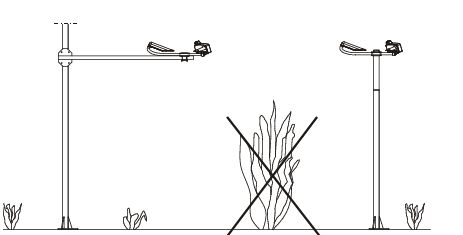
\includegraphics[width=0.75\textwidth]{images/loc.png}
    \caption{Recommended installation site criteria for PWD sensors (see PWD12 Manual\cite{vaisala2015pwd}, Chapter 4)}
    \label{fig:siteguidelines}
\end{figure}

\subsection{Mounting Orientation and Positioning}

The \gls{pwd12} is typically mounted on a vertical pole or mast using Vaisala's dedicated mounting kit\cite{vaisala2015pwd} or a compatible adapter. The optical head must remain perfectly horizontal during operation to avoid distortion in visibility measurement. The mounting setup should ensure:

\begin{itemize}
    \item A fixed, stable structure such as a mast or rail.
    \item Horizontal alignment of the sensor body and unobstructed view of the measurement volume.
    \item To avoid sunlight or artificial light interference, the optics should not face strong light sources.
    \item In the northern hemisphere, the \textbf{receiver should be oriented toward the north}, while in the southern hemisphere it should face south.
\end{itemize}

\subsection{Grounding and Surge Protection}

Electrical protection is essential, especially in outdoor installations exposed to lightning or power surges. Vaisala recommends the following protection measures\cite{vaisala2015pwd}:

\begin{itemize}
    \item The \gls{pwd12} sensor chassis must be \textbf{properly grounded} to earth using a dedicated grounding wire.
    \item A Vaisala \textbf{lightning protection device} should be installed in-line between the power source and the sensor, especially in high-risk areas.
    \item Shielded cables and grounded cable armor are recommended to further suppress electromagnetic interference.
\end{itemize}

Failing to implement grounding and surge protection can compromise both safety and long-term sensor performance.



\section{Electrical Wiring and Communication Interfaces}

The \gls{pwd12} sensor requires careful attention during electrical integration to ensure reliable communication and power delivery. This includes proper pin-out matching, interface selection, cable shielding, and adherence to electrical specifications. For complete wiring specifications, see the Vaisala PWD12 User Manual, Section 4.2\cite{vaisala2015pwd}.

\subsection{Pin-out and Wire Color Mapping}

The sensor is delivered with a fixed 16-wire cable, which provides lines for power, serial communication, relay outputs, and diagnostics. Table~\ref{tab:pwd12pins} shows the color mapping of the 16 wires in the \gls{pwd12} cable, the function of each wire, and the assigned pin:

\begin{table}[H]
\small
\renewcommand{\arraystretch}{1.5}
\centering
\caption{Recommended Pin-out Connections for Basic Operation}
\label{tab:pwd12pins}
\begin{tabular}{|c|l|l|}
\hline
\textbf{Wire Color} & \textbf{Function} & \textbf{Pin} \\
\hline
Red     & Power +24 VDC & 1 \\
\hline
Black   & Power GND     & 2 \\
\hline
White   & RS-485 B (-)     & 3 \\
\hline
Brown    & RS-485 A (+)     & 4 \\
\hline
Green    & RS-232 Tx      & 5 \\
\hline
Yellow  & RS-232 Rx  & 6 \\
\hline
Grey     & RS-232 GND & 7 \\
\hline
Blue   & Analog Output     & 8 \\
\hline
White/Green   & Heating Power +     & 9 \\
\hline
Brown/Green    & Heating Power +     & 10 \\
\hline
White/Yellow    & Heating Power -      & 11 \\
\hline
Brown/Yellow  & Heating Power -  & 12 \\
\hline
Grey/Pink   & Relay Control 1     & 13 \\
\hline
Red/Blue    & Relay Control 2     & 14 \\
\hline
Violet    & Relay Control 3 / Ext Vb      & 15 \\
\hline
Pink  & Ext Vb  & 16 \\
\hline
\end{tabular}
\end{table}

Figure~\ref{fig:pwd12pinouts} shows the full 16-pin connector layout that should be used in this installation.

\begin{figure}[H]
\centering
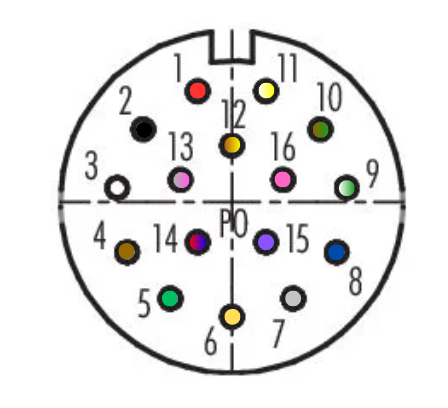
\includegraphics[width=0.4\textwidth]{images/16pins.png}
\caption{\gls{pwd12} cabling overview: 16-wire original mapping}
\label{fig:pwd12pinouts}
\end{figure}

\subsection{Supported Communication Interfaces}
\label{sec:pwd12wiring}

The \gls{pwd12} supports two digital communication interfaces:

\begin{itemize}
    \item \textbf{\gls{rs485} (default):} Full-duplex, differential communication. Recommended for long distances and electrically noisy environments. Baud rate: \textbf{9600}, \textbf{7 data bits}, \textbf{even parity}, \textbf{1 stop bit}.
    \item \textbf{\gls{rs232} (optional):} Used primarily for manual configuration and diagnostics. Requires a \gls{usb}–\gls{rs232} converter and a terminal emulator on the host device.
\end{itemize}

\textbf{RS-485 was selected for this integration} due to its superior resistance to electromagnetic interference, support for longer cable runs, and compatibility with existing RevPi serial interfaces. RS-232 was used only during initial bench testing and manual configuration.

\subsection{Cable Shielding and Length Constraints}

To ensure stable signal quality and \gls{emi} protection:

\begin{itemize}
    \item Use shielded twisted pair cables for \gls{rs485} signals.
    \item The cable shield (bare wire) should be grounded at the panel side only.
    \item Keep the communication cable length under \textbf{1,200 meters} for \gls{rs485}, as per standard limitations.
    \item Ensure separation between power lines and communication lines to reduce noise coupling.
\end{itemize}

These precautions improve data integrity and prevent \gls{crc} parsing errors in electrically noisy or outdoor environments\cite{vaisala2015pwd}.



\section{Sensor Configuration and Command Structure}

The Vaisala \gls{pwd12} sensor offers flexible configuration through a serial interface, primarily using \gls{rs232} for direct command access. Most configuration and diagnostic operations are executed in \textit{command mode}. The required serial parameters were outlined in Section~\ref{sec:pwd12wiring}, and this section focuses on the command protocol and available setup options.

During integration, the default settings were largely sufficient. Only minor adjustments were made to the output format (Message 2/7 selection), output interval, and filtering level using documented commands. All commands follow the syntax and descriptions provided in the Vaisala \gls{pwd12} User Manual (e.g., Section 7.3)\cite{vaisala2015pwd}.

\subsection{Command Mode and Access}

To access command mode via \gls{rs232}, the following command must be sent:

\begin{center}
    \texttt{OPEN *}
\end{center}

Once command mode is active, the sensor accepts \gls{ascii}-based instructions. All commands must be terminated with a carriage return (CR, \texttt{0x0D}). The sensor replies with either confirmation messages or returned data strings depending on the command type.

\subsection{Configuration and Setup Commands}

Table~\ref{tab:pwd12commands_config} summarizes common setup commands used to control sensor behavior and output characteristics.

\begin{table}[H]
\centering
\small
\renewcommand{\arraystretch}{1.4}
\caption{PWD12 Configuration Commands (see PWD12 Manual\cite{vaisala2015pwd}, Chap. 5)}
\label{tab:pwd12commands_config}
\begin{tabular}{|l|p{9cm}|}
\hline
\textbf{Command} & \textbf{Description} \\
\hline
\texttt{WSET} & View or modify weather message type and code format (NWS/WMO). \\
\hline
\texttt{SSET} & Configure output interval, filtering, and enabled parameters (e.g., temperature, luminance). \\
\hline
\texttt{CLRS} & Clear accumulated rain and snow measurements. Used at installation or reset. \\
\hline
\texttt{WPAR} & Display current weather-related parameters such as visibility, precipitation thresholds. \\
\hline
\texttt{MSG} & Select which output messages to emit (e.g., Message 2 or Message 7). \\
\hline
\end{tabular}
\end{table}

\subsection{Calibration and RAINCAP Adjustment}

The RAINCAP sensor can be recalibrated if necessary. Table~\ref{tab:pwd12commands_calibration} lists relevant commands.

\begin{table}[H]
\centering
\small
\renewcommand{\arraystretch}{1.4}
\caption{PWD12 RAINCAP Calibration Commands (see PWD12 Manual\cite{vaisala2015pwd}, Chap. 5)}
\label{tab:pwd12commands_calibration}
\begin{tabular}{|l|p{9cm}|}
\hline
\textbf{Command} & \textbf{Description} \\
\hline
\texttt{DRY ON} & Set reference level for no precipitation. Run when the sensor is dry. \\
\hline
\texttt{WET ON} & Set reference level for active precipitation. Run during rain. \\
\hline
\texttt{DRY} / \texttt{WET} & Read current dry/wet calibration status and thresholds. \\
\hline
\end{tabular}
\end{table}

\subsection{Diagnostic and Status Commands}

The sensor provides various commands to monitor internal status and ensure healthy operation:

\begin{table}[H]
\centering
\small
\renewcommand{\arraystretch}{1.4}
\caption{PWD12 Status and Diagnostic Commands (see PWD12 Manual\cite{vaisala2015pwd}, Chap. 5)}
\label{tab:pwd12commands_diag}
\begin{tabular}{|l|p{9cm}|}
\hline
\textbf{Command} & \textbf{Description} \\
\hline
\texttt{STAT} & Returns internal status and error flags. \\
\hline
\texttt{TEMP} & Displays current internal and ambient temperatures. \\
\hline
\texttt{IDN?} & Query the sensor’s model ID, firmware version, and serial number. \\
\hline
\end{tabular}
\end{table}

These diagnostic tools support field validation, health monitoring, and automated sensor management. Most of the commands listed above are covered in Section 7.3 and Appendix A of the PWD12 User Manual.

\paragraph{}%
Wherever possible, configuration changes were minimized to preserve factory-calibrated accuracy. The default Message 2 format and 15-second output interval proved sufficient for integration with the RevPi data pipeline and downstream GraphQL schema.


\section{Sensor Testing and Message Validation}

To ensure proper functionality and compatibility of the \gls{pwd12} sensor before integration into the operational weather station, it is essential to carry out standalone testing. This includes establishing a communication link, analyzing output message formats, and validating that all expected parameters are correctly reported and parsable.

\subsection{Bench Setup and Mock Communication}

For standalone testing outside of the field deployment, the \gls{pwd12} was connected to a controlled bench setup using a regulated laboratory power supply and a USB–RS485 converter attached to a development laptop. This allowed direct communication with the sensor before integrating it into the RevPi system.

The external power supply delivered 24\,V\,DC, sufficient to power the measurement electronics. Only the essential lines from the PWD12 16-wire cable were connected: power (red/black) and the differential pair for RS-485 communication (brown/white). The heaters and additional auxiliary lines were not used in this configuration.

Table~\ref{tab:pwd12benchpins} summarizes the connections made during the bench setup.

\begin{table}[H]
\renewcommand{\arraystretch}{1.6}
\centering
\small
\caption{Pin-out connections used for bench testing}
\label{tab:pwd12benchpins}
\begin{tabular}{|l|l|}
\hline
\textbf{PWD12 Wire Color} & \textbf{Function} \\
\hline
Red   & Power +24 VDC \\
\hline
Black & Power GND \\
\hline
Brown & RS-485 A (+) \\
\hline
White & RS-485 B (–) \\
\hline
\end{tabular}
\end{table}

Figure~\ref{fig:pwd12benchsetup} illustrates the simplified bench setup, showing the PWD12 sensor connected to the external power supply and to a laptop via USB–RS485 converter.

\begin{figure}[H]
  \centering
  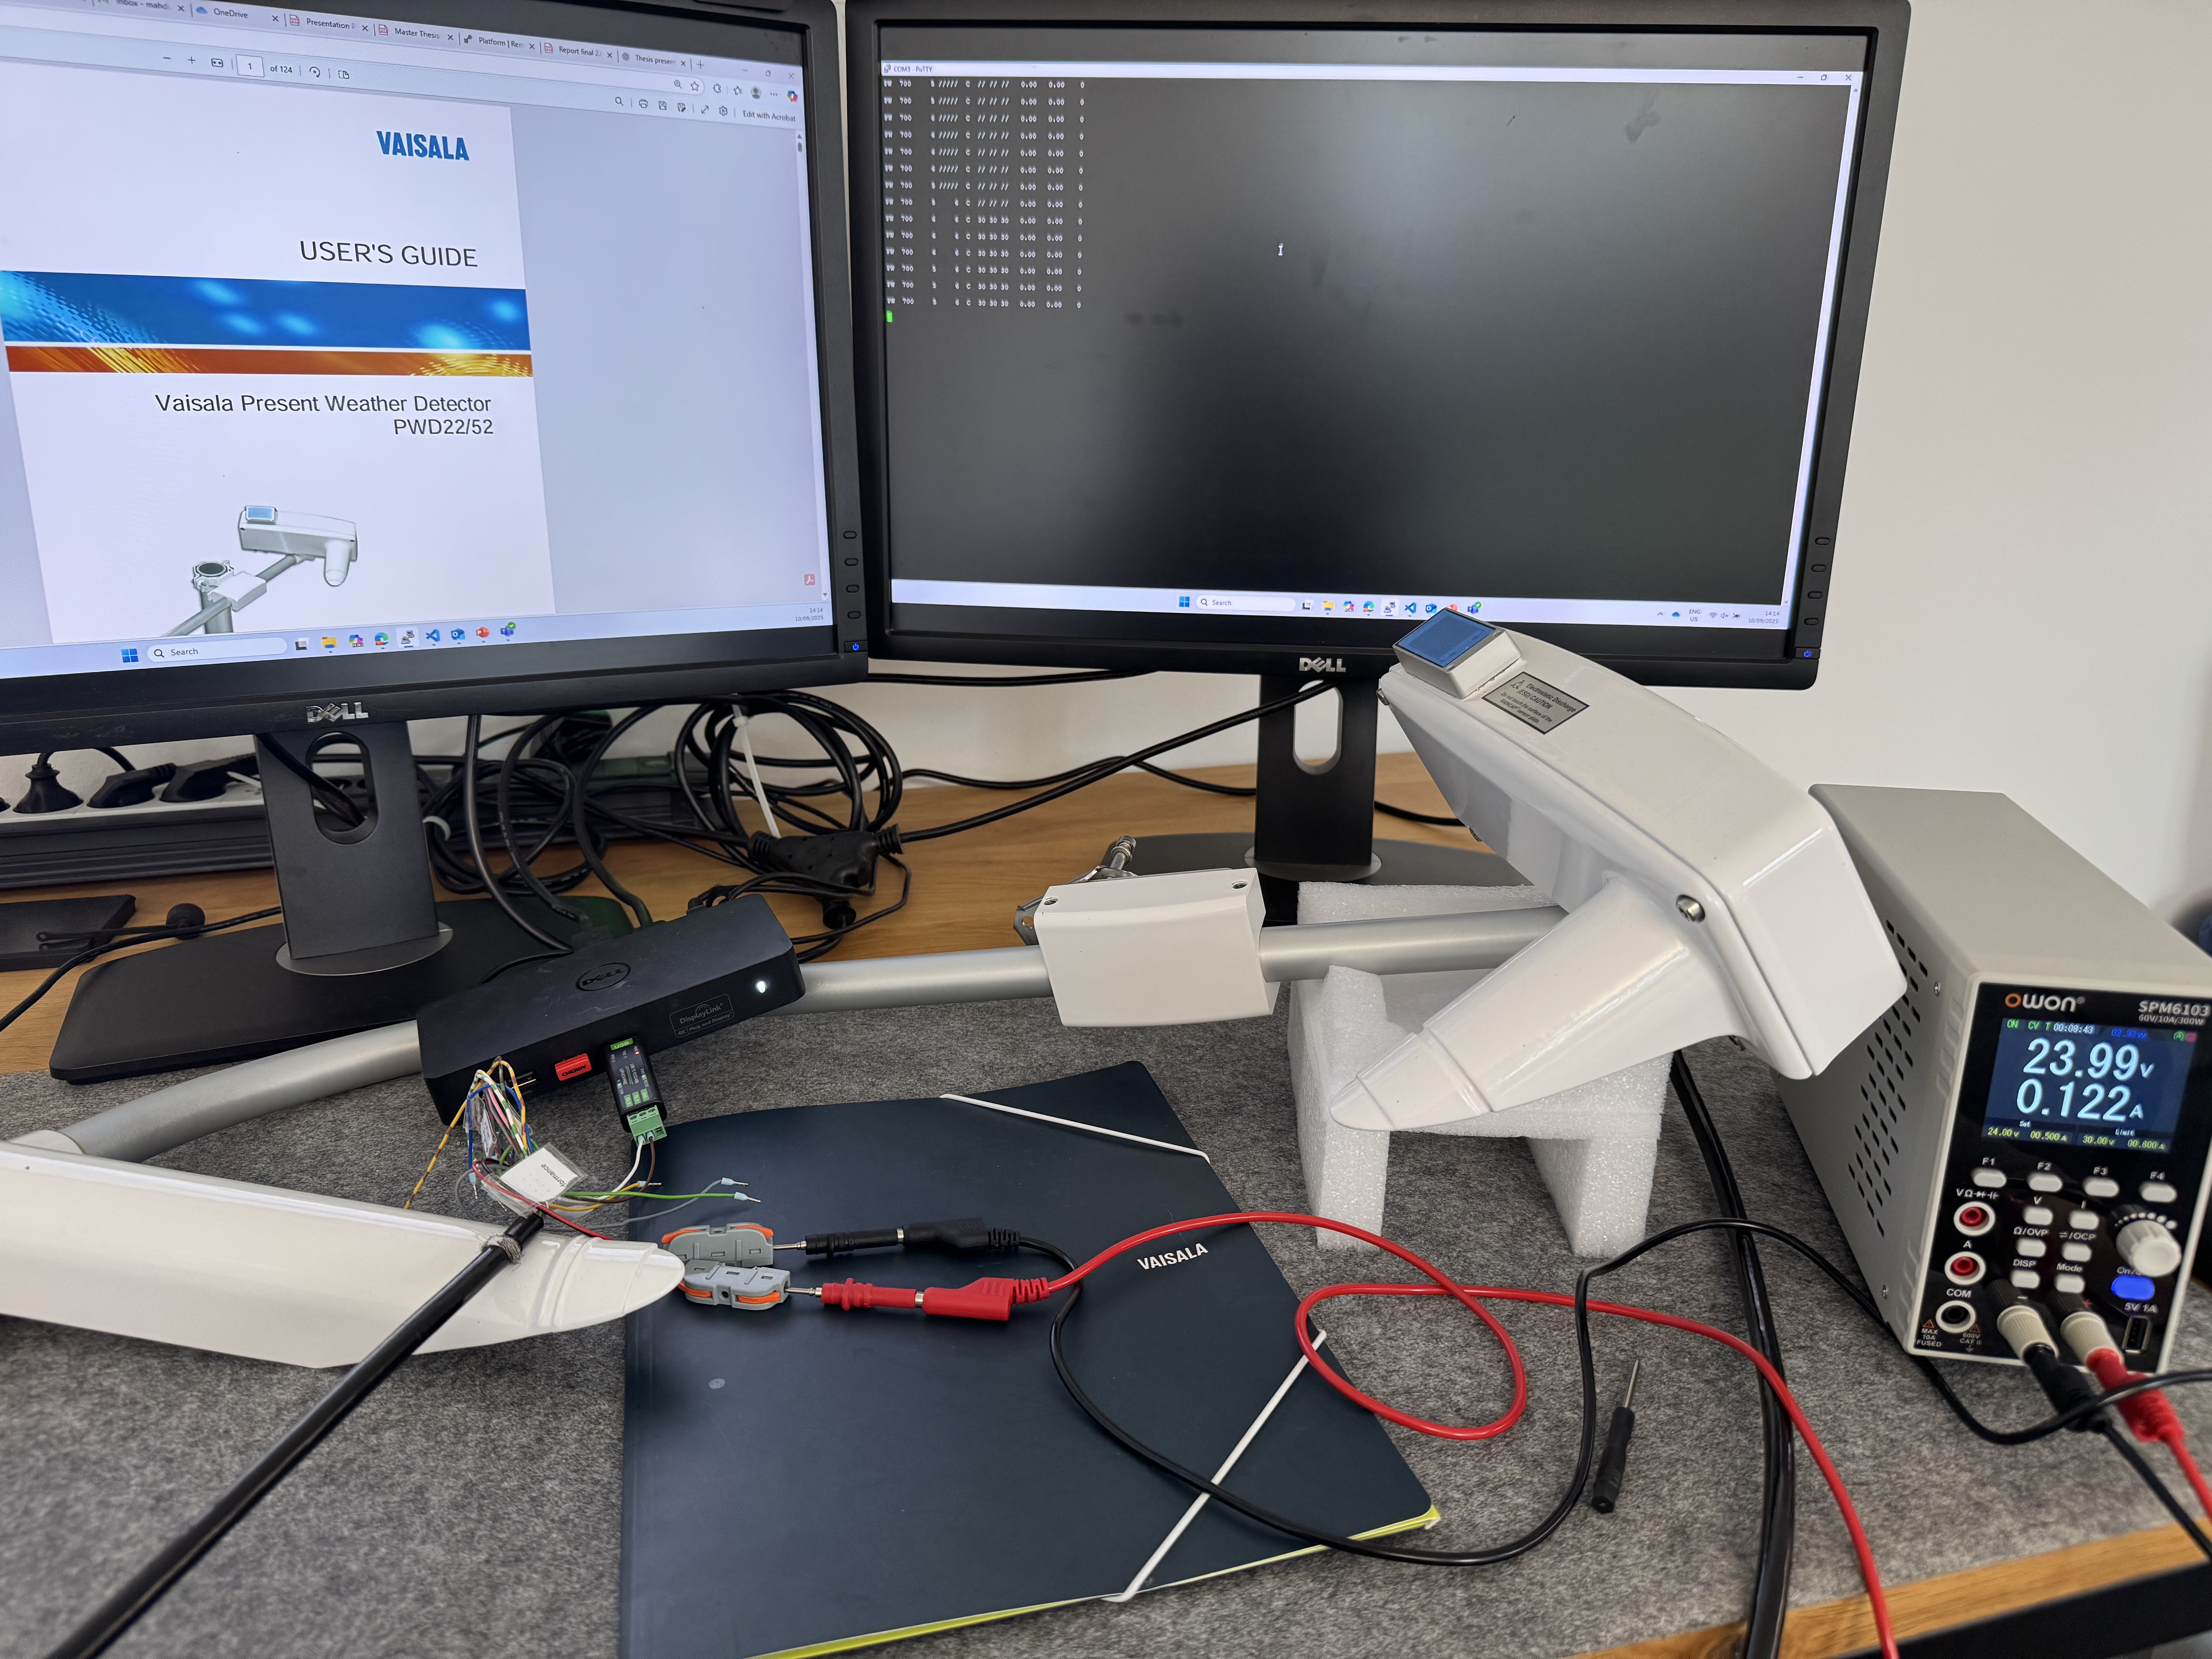
\includegraphics[width=0.7\textwidth]{images/pwd12_bench_setup.jpg} % <-- replace with your schematic
  \caption{Bench testing setup: PWD12 connected to external PSU and USB–RS485 converter}
  \label{fig:pwd12benchsetup}
\end{figure}

% \begin{table}[H]
% \renewcommand{\arraystretch}{1.8}
% \centering
% \caption{Pin-out Connections used for testing}
% \label{tab:pwd12testpins}
% \begin{tabular}{|c|l|l|l|}
% \hline
% \textbf{Wire Color} & \textbf{Function} & \textbf{M12 Pin} & \textbf{PWD12 Wire Color} \\
% \hline
% White     & ---                 & 1 & --- \\
% \hline
% Brown     & Power +24 VDC       & 2 & Red \\
% \hline
% Green     & ---                 & 3 & --- \\
% \hline
% Yellow    & ---                 & 4 & --- \\
% \hline
% Grey      & \gls{rs485} A (+)   & 5 & Brown \\
% \hline
% Pink      & ---                 & 6 & --- \\
% \hline
% Blue      & \gls{rs485} B (-)   & 7 & White \\
% \hline
% Red       & Power GND           & 8 & Black \\
% \hline
% \end{tabular}
% \end{table}

% Figure~\ref{fig:pwd12bench} shows the simplified 8-pin M12 connector layout used in the test bench.

% \begin{figure}[H]
%   \centering
%   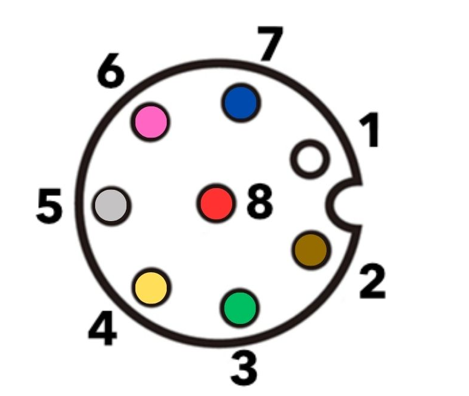
\includegraphics[width=0.5\textwidth]{images/8pins.png}
%   \caption{Simplified 8-pin wiring used for bench setup}
%   \label{fig:pwd12bench}
% \end{figure}

Before switching to VS Code, data was monitored using a terminal emulator (\texttt{Putty}), with serial settings matching the \gls{pwd12} specification: 9600 baud, 7 data bits, even parity, and 1 stop bit.

\subsection{Message Format Verification and Sensor Behavior}

Once powered and initialized, the \gls{pwd12} begins periodically transmitting data via the \gls{rs485} interface. By default, this output is in Message 2 format, which includes visibility readings, present weather codes, and precipitation data.

A representative message output is shown below:

\begin{verbatim}
PW 100 1839 1505 C 61 61 61 0.33 12.16 0
\end{verbatim}

Each field in the message corresponds to a specific parameter:

\begin{itemize}
  \item \texttt{PW} — Sensor prefix
  \item \texttt{1} — Sensor unit ID
  \item \texttt{00} — Status code
  \item \texttt{1839} — 1-minute average visibility (m)
  \item \texttt{1505} — 10-minute average visibility (m)
  \item \texttt{C} — Instant present weather (\gls{nws} code)
  \item \texttt{61, 61, 61} — Instant, 15-min, and 1-hour \gls{wmo} \gls{synop} weather codes
  \item \texttt{0.33} — Precipitation intensity (mm/h)
  \item \texttt{12.16} — Cumulative water sum (mm)
  \item \texttt{0} — Cumulative snow sum (mm)
\end{itemize}

During testing, this message was confirmed to:

\begin{itemize}
  \item Be emitted at the expected interval (typically every 15 seconds)
  \item Contain no malformed syntax or communication errors
  \item Include all expected measurement fields
\end{itemize}

\subsection{Raw Message Interpretation and Field Mapping}

To ensure compatibility with downstream processing and the cloud API, a dedicated Python parser was implemented to interpret raw messages. The parser handled:

\begin{itemize}
  \item Serial readout and newline stripping
  \item Splitting by whitespace
  \item Assigning each field to a semantically meaningful key
  \item Type validation (e.g., casting to float or integer)
\end{itemize}


\subsection{Final JSON Structure and Cloud Compatibility}

The parsed fields are serialized into a structured \gls{json} object as follows:

\begin{lstlisting}[language=json, caption={Parsed JSON structure from raw PWD12 message}, label={lst:parsedjson}]
{
  "sensor_id": "PW7",
  "visibility_alarm": "No Alarm",
  "status_code": "No hardware error",
  "visibility_1min": 1839,
  "visibility_10min": 1505,
  "present_weather_nws": "Light Rain",
  "present_weather_code_inst": "Rain",
  "present_weather_code_15min": "Rain",
  "present_weather_code_1h": "Rain",
  "precip_intensity": 0.33,
  "precip_cumulative": 12.16,
  "snow_sum": 0
}
\end{lstlisting}

This structure aligns with the expected GraphQL schema and supports direct ingestion by the cloud backend. The translation from \gls{wmo} and \gls{nws} codes to descriptive weather types is handled using predefined mapping tables.

Figure~\ref{fig:pwd12-raw-json} illustrates the transformation result: 
a raw ASCII message from the PWD12 sensor is parsed into a structured JSON object, 
aligning with the cloud schema for direct ingestion.

\begin{figure}[H]
  \centering
  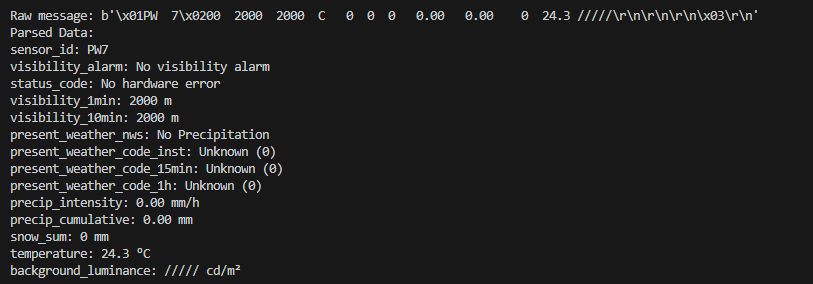
\includegraphics[width=\textwidth]{images/pwd12_raw_vs_json.png} % <-- your screenshot
  \caption{Example of a raw PWD12 message and the corresponding parsed JSON structure.}
  \label{fig:pwd12-raw-json}
\end{figure}


Additional parser logic ensures graceful failure handling for:

\begin{itemize}
  \item Incomplete messages or field truncation
  \item Unexpected data types
  \item Out-of-range values
\end{itemize}

This structured pipeline guarantees that data entering the cloud is both semantically valid and consistent across all weather stations.


\section*{Conclusion}

This chapter provided a comprehensive study of the Vaisala \gls{pwd12} sensor, outlining its measurement principles, internal components, technical specifications, and operational requirements. Particular emphasis was placed on understanding the optical forward-scatter method for visibility estimation, the RAINCAP precipitation detection system, and the role of integrated heating and protective mechanisms in ensuring continuous operation under harsh weather conditions.

Through standalone bench testing, the sensor’s communication interface and output format were successfully verified. Raw ASCII messages were captured, parsed, and transformed into structured JSON objects, demonstrating compatibility with downstream data handling pipelines. The tests confirmed that the sensor reliably outputs visibility, precipitation, and present weather codes at the expected intervals, with no communication errors or malformed data.

By establishing both the theoretical background and practical validation of the sensor’s output, this study laid the groundwork for its integration into the operational weather station. The findings ensure confidence that the \gls{pwd12} can extend the system’s capabilities with accurate visibility data, thereby supporting weather-aware flight monitoring and vertiport operations. The next chapter builds on these results by addressing the integration process, covering the hardware wiring, software architecture, and cloud connectivity required to deploy the sensor in the field.

\cleardoublepage



\setlength{\headheight}{27.41803pt}
\chapter{Integration of the PWD12 Sensor into the Weather Station}

\section*{Introduction}

This chapter details the integration process of the Vaisala \gls{pwd12} visibility sensor into the existing weather station system, which already featured a Vaisala WXT536 for meteorological data collection. The integration covered both hardware and software aspects, requiring careful adaptation of the system architecture to support a second sensor with different communication and data characteristics. Emphasis is placed on maintaining modularity, ensuring system reliability, and enabling cloud connectivity through AWS services. The integration not only enhances the scope of environmental data collected, particularly in terms of visibility and present weather conditions, but also strengthens the platform’s value for Unisphere’s flight monitoring and \gls{uas} operations. Each section of this chapter walks through the technical steps, challenges, and solutions involved in enabling seamless communication, data acquisition, offline buffering, and cloud synchronization for the new sensor.

\section{System Architecture and Data Flow}

\subsection{Revised Hardware and Software Stack Overview}

With the integration of the Vaisala \gls{pwd12} sensor, the weather station now incorporates two separate sensing units: the existing WXT536 for core weather measurements and the \gls{pwd12} for visibility and present weather detection. Both sensors are physically connected to the same \gls{revpi} device using dedicated \gls{rs485} serial interfaces. The WXT536 operates at 19200~bps while the \gls{pwd12} uses 9600~bps, which necessitates independent communication ports for reliable operation.

In terms of cabling, the PWD12 is connected to the RevPi through its 8-pin M12 connector. 
Only the essential lines are used: the power supply (24 V DC) and the RS-485 differential 
pair for serial communication. Optional connections such as heater power or analog outputs 
were not required in this deployment and were therefore left unconnected.

Table~\ref{tab:pwd12integrationpins} summarizes the wiring used for the integration, 
while Figure~\ref{fig:pwd12integration} illustrates the simplified pinout layout of the 
8-pin connector as implemented in the weather station.

\begin{table}[H]
\renewcommand{\arraystretch}{1.8}
\centering
\small
\caption{Pin-out connections used for PWD12 integration into the weather station}
\label{tab:pwd12integrationpins}
\begin{tabular}{|c|l|l|l|}
\hline
\textbf{M12 Pin} & \textbf{Wire Color (Cable)} & \textbf{Function} & \textbf{PWD12 Internal Wire} \\
\hline
2 & Brown   & +24 V DC Power & Red \\
\hline
5 & Grey    & RS-485 A (+)   & Brown \\
\hline
7 & Blue    & RS-485 B (-)   & White \\
\hline
8 & Red     & Power GND      & Black \\
\hline
\end{tabular}
\end{table}


\begin{figure}[H]
  \centering
  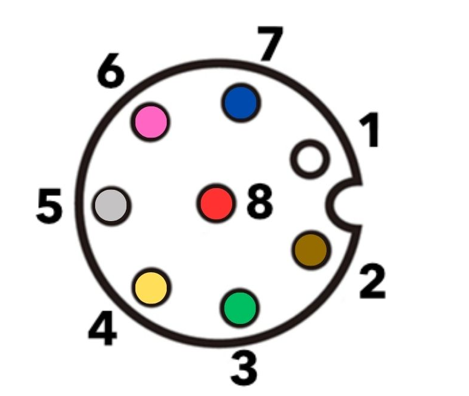
\includegraphics[width=0.45\textwidth]{images/8pins.png}
  \caption{Simplified 8-pin wiring for PWD12 integration into the weather station}
  \label{fig:pwd12integration}
\end{figure}

On the software side, the architecture retains its modular design. Each sensor is handled by its own Python module, responsible for reading, parsing, and structuring messages. These modules run in parallel threads within a single systemd-managed process, ensuring fault isolation and efficient concurrency.

Figure~\ref{fig:hardware_architecture} presents the Updated hardware architecture of the weather station after \gls{pwd12} integration, showing the \gls{revpi} Connect+, dual \gls{rs485} connections (WXT536 and \gls{pwd12}), and supporting power supply.

\begin{figure}[H]
  \centering
  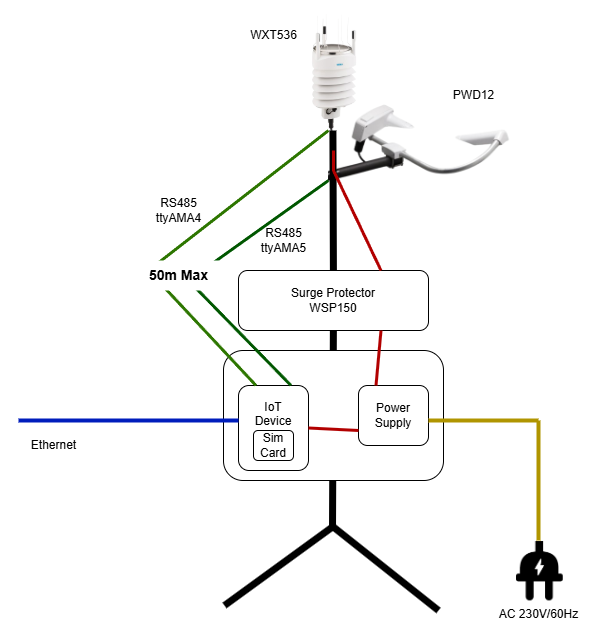
\includegraphics[width=0.75\textwidth]{images/hardware_architecture.png}
  \caption{Revised hardware setup}
  \label{fig:hardware_architecture}
\end{figure}

\subsection{Local Communication and Parsing Workflow}

At the local level, the \gls{revpi} handles real-time communication with both the \gls{pwd12} and WXT536 sensors via two separate \gls{rs485} ports. Each sensor's data stream is processed independently through dedicated reader and parser modules, which are initialized in separate threads within a single Python process managed by systemd. This design ensures that failures in one sensor's parsing logic do not interfere with the operation of the other.

The reader modules continuously monitor their respective serial interfaces, decoding messages based on predefined formats. After basic validation, the data is passed to parser modules that extract relevant fields such as visibility, precipitation, wind speed, or atmospheric pressure. Parsed messages are then structured into unified \texttt{\gls{json}}-like dictionaries and passed downstream for cloud transmission or local buffering.

This modular threading architecture allows for concurrent execution while keeping the codebase maintainable and sensor logic loosely coupled. Figure~\ref{fig:revpi_data_flow} summarizes the local data flow within the \gls{revpi}: independent serial reading threads parse WXT536 and \gls{pwd12} messages into structured \gls{json} dictionaries for either cloud upload or local buffering.

\begin{figure}[H]
  \centering
  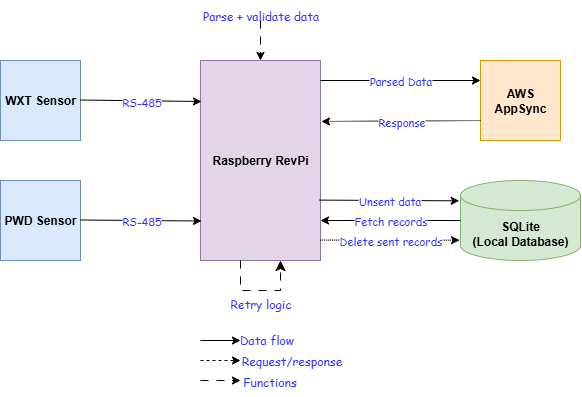
\includegraphics[width=0.7\textwidth]{images/RevPi_data_flow.png}
  \caption{Data flow within the \gls{revpi}: from sensor input to message parsing and output}
  \label{fig:revpi_data_flow}
\end{figure}

\subsection{Cloud Transmission Pipeline and AWS Integration}

Once data is parsed and structured locally, it is transmitted to the cloud via a GraphQL \gls{api} exposed by \gls{aws} appsync. Both the \gls{pwd12} and WXT536 sensors share the same endpoint, with each message tagged by a sensor-specific identifier to allow differentiation on the backend. This unified interface simplifies the cloud integration and reduces the need for multiple endpoints or \gls{api} configurations.

The cloud pipeline relies on \gls{aws} AppSync as the main entry point, forwarding validated messages to a DynamoDB table for temporary storage and to backend services such as Lambda for further processing.

This design enables near real-time access to weather and visibility data while maintaining flexibility for downstream analytics or alerting procedures. The structure also supports asynchronous operations like offline buffering and retry mechanisms, which are detailed later in Section~\ref{sec:offline-buffering}.

\section{Codebase Structure and Development Environment}
\label{sec:codebase-structure}

\subsection{Programming Environment and Tools Used}

The weather station system is developed in \textbf{Python 3.11} and runs on \textbf{Raspberry Pi OS (Bookworm)} installed on the RevPi Connect+. This environment offers a stable and flexible base, with full support for modern Python features and libraries. 

The system relies on a minimal set of external dependencies, declared in a dedicated \texttt{requirements.txt} file. These include modules for serial communication, environment variable loading, GraphQL API interaction, and \gls{json} processing. In addition, runtime and deployment are supported by standard Linux services and external tools for version control and remote management. 

Table~\ref{tab:tools} summarizes the key tools and technologies used, organized by category to reflect their different roles in the system.


\begin{table}[H]
\centering
\small
\caption{Key development tools and technologies}
\label{tab:tools}
\begin{tabular}{|p{5cm}|p{3cm}|p{7.5cm}|}
\hline
\textbf{Category} & \textbf{Tool} & \textbf{Function} \\
\hline
Python Libraries & \texttt{pyserial} & Serial port communication \\
 & \texttt{requests} & HTTP-based GraphQL communication \\
 & \texttt{python-dotenv} & Environment variable loading \\
\hline
System \& Runtime Tools & \texttt{systemd} & Persistent background service management \\
\hline
Deployment \& Remote Management & \texttt{git} & Version control and deployment \\
 & \texttt{Qbee} & Remote access, configuration, and logging \\
\hline
\end{tabular}
\end{table}


\subsection{Folder Layout and Modularization Approach}

The codebase is organized in a modular structure to improve clarity, reusability, and separation of concerns. Each sensor has its own folder containing the core scripts for reading and parsing serial messages. Shared utilities such as offline buffering or main orchestration logic reside in the project root directory.
{\small
\begin{lstlisting}[language=bash,caption={Project folder layout (simplified)},label={lst:folder-structure-ascii}]
    weather_station/
|- docs
|  |- images
|  |- sensor_installation.md
|  |- sensor_specifications.md
|  \- system_architecture.md
|- pwd12/
|  |- error_handler.py
|  |- parser.py
|  \- reader.py
|- wxt536/
|  |- checksum_handler.py
|  |- parser.py
|  \- reader.py
|- buffer_manager.py
|- main.py
|- data_structure.md
|- env_var.env
|- README.md
|- requirements.txt
\- .gitignore
\end{lstlisting}
}



This separation allows sensor-specific logic to be maintained independently, with minimal coupling. Shared logic such as error handling or buffering is centralized to prevent duplication.

\subsection{Environment Variable Management and Secrets Handling}

To avoid hardcoding sensitive information such as \gls{api} keys and serial port paths, the system loads its configuration from a \texttt{.env} file using the \texttt{python-dotenv} package. This approach enables secure and flexible deployments, especially when using version control.
{\small
\begin{lstlisting}[language=bash,caption={Example .env file entries},label={lst:.env}]
APPSYNC_ENDPOINT=https://your-api.appsync-api.amazonaws.com/graphql
APPSYNC_API_KEY=your-secret-key
PWD_ID=IPC2100_PWD12
WXT_ID=IPC2100_WXT536
WXT_PORT=/dev/ttyAMA4
PWD_PORT=/dev/ttyAMA5
\end{lstlisting}
}
These variables are injected at runtime and accessed by the code using standard environment access functions, providing a clean interface between configuration and logic.



\section{Data Acquisition Pipeline}
\label{sec:data_pipeline}

This section describes how sensor data from the WXT536 and \gls{pwd12} devices is acquired, parsed, and structured locally before being forwarded to cloud infrastructure or buffered during offline periods.

\subsection{Serial Port Communication}

The two sensors communicate independently over dedicated \gls{rs485} interfaces, each connected to its own serial port on the \gls{revpi}. The WXT536 operates at 19200 baud with 8 data bits and no parity, while the \gls{pwd12} uses 9600 baud, 7 data bits, even parity, and one stop bit. Serial port parameters are explicitly set using Python's \texttt{pyserial} library at runtime.

The \gls{pwd12} line reader opens the port using environment variables (via \texttt{dotenv}) and waits for newline-terminated messages in blocking mode. The WXT536 reader uses a higher-level class, \texttt{WXT530ASCII}, to issue ASCII-based polling requests and receive either composite or multi-line data messages. Each read loop runs in its own thread, continuously reading and timestamping data from the corresponding port.

\subsection{Message Parsing and Error Handling}

Once data is read from the serial port, each message is validated and parsed.

\begin{itemize}
    \item \textbf{WXT536}: Each multi-line response is parsed individually using a checksum validation function before converting key-value pairs into a structured dictionary. Custom mappings translate sensor codes (e.g., \texttt{Sm=}, \texttt{Ta=}) into descriptive field names like \texttt{wind\_speed\_average} and \texttt{air\_temperature}.
    \item \textbf{\gls{pwd12}}: Each line is first validated for structure and length using a dedicated validator. The parser decodes the byte stream, filters control characters, and maps numeric fields to visibility, precipitation, and present weather codes. External lookup dictionaries are used for translating \gls{nws} character codes and \gls{wmo} numeric codes into human-readable weather descriptions.
\end{itemize}

Errors such as malformed lines, invalid values, or checksum mismatches are logged and do not crash the main pipeline. For the WXT536, retry logic is included to tolerate transient checksum failures (up to 3 attempts).

Figure~\ref{fig:flow-acquisition} illustrates this parsing and validation workflow step by step.

%%%%%%%%%%%%%%%%%%%%%%%%%%%%%%%%%%%%%%%%
% 1. Sensor Data Acquisition
%%%%%%%%%%%%%%%%%%%%%%%%%%%%%%%%%%%%%%%%
\begin{figure}[H]
\centering
\begin{adjustbox}{width=0.8\textwidth}
\begin{tikzpicture}[node distance=2cm]
\node (start) [startstop] {Start};
\node (read) [process, below of=start] {Read serial message from sensor};
\node (check) [decision, below of=read, yshift=-0.5cm] {Valid message?};
\node (discard) [process, right of=check, xshift=6cm] {Discard message};
\node (parse) [process, below of=check, yshift=-2.5cm] {Parse and structure data};
\node (end) [startstop, below of=parse] {Pass to buffering/transmission};

\draw [arrow] (start) -- (read);
\draw [arrow] (read) -- (check);
\draw [arrow] (check.east) -- ++(2,0) -- (discard.west) node[midway, above]{No};
\draw [arrow] (check.south) -- ++(0,-1.3) -- (parse.north) node[midway, right]{Yes};
\draw [arrow] (parse) -- (end);
\end{tikzpicture}
\end{adjustbox}
\caption{Logigram of sensor data acquisition and validation workflow.}
\label{fig:flow-acquisition}
\end{figure}

\subsection{Schema Mapping and Output Structuring}

After parsing, both sensor data dictionaries are augmented with metadata (such as timestamp and sensor ID) and prepared for transmission. The schema used internally aligns with the backend cloud structure and is converted to \gls{json} before being passed to the GraphQL mutation.

For example, a sample output from the PWD12 parser might be structured as shown in Listing~\ref{lst:pwd12-json}.
{\small
\begin{lstlisting}[language=json, caption={Parsed JSON structure from a PWD12 message}, label={lst:pwd12-json}]
{
  "visibility_alarm": "No Alarm",
  "visibility_1min": 1839,
  "visibility_10min": 1505,
  "present_weather_nws": "Light Rain",
  "present_weather_code_inst": "Rain",
  "present_weather_code_15min": "Rain",
  "present_weather_code_1h": "Rain",
  "precip_intensity": 0.33,
  "precip_cumulative": 12.16,
  "snow_sum": 0
}
\end{lstlisting}

}

This structured representation is then either transmitted directly to \gls{aws} AppSync or stored in a local SQLite buffer in case of network unavailability, as described in Section~\ref{sec:offline-buffering}.

The decision process between cloud transmission and local buffering is shown in Figure~\ref{fig:flow-buffering}.

%%%%%%%%%%%%%%%%%%%%%%%%%%%%%%%%%%%%%%%%
% 2. Offline Buffering
%%%%%%%%%%%%%%%%%%%%%%%%%%%%%%%%%%%%%%%%
\begin{figure}[H]
\centering
\begin{tikzpicture}[node distance=2cm]
\node (start) [startstop] {Incoming parsed data};
\node (netcheck) [decision, below of=start, yshift=-0.5cm] {Internet available?};
\node (sqlite) [process, right of=netcheck, xshift=6cm] {Store in local SQLite database};
\node (push) [process, below of=netcheck, yshift=-1.5cm] {Send directly to cloud (AppSync)};
\node (end) [startstop, below of=push] {Done};

\draw [arrow] (start) -- (netcheck);
\draw [arrow] (netcheck.east) -- ++(2,0) -- (sqlite.west) node[midway, above]{No};
\draw [arrow] (netcheck.south) -- ++(0,-1.3) -- (push.north) node[midway, right]{Yes};
\draw [arrow] (push) -- (end);
\end{tikzpicture}
\caption{Logigram of offline buffering with SQLite.}
\label{fig:flow-buffering}
\end{figure}


\section{Offline Buffering and Local Data Resilience}
\label{sec:offline-buffering}

\subsection{Problem Statement and Design Requirements}

In deployments where cellular connectivity may be unstable or unavailable for long durations, the weather station must guarantee data integrity by buffering locally. The buffering mechanism must:

\begin{itemize}
    \item Store all sensor data during internet outages without loss
    \item Automatically retry sending once connectivity is restored
    \item Prevent duplicated uploads
    \item Limit storage usage and clean up old entries if necessary
\end{itemize}

\subsection{Evaluation of Local Storage Options}

Several local buffering mechanisms were considered for storing sensor data during internet outages. Table~\ref{tab:buffering_comparison} summarizes the trade-offs:

\begin{table}[H]
\centering\
\small
\caption{Local storage option comparison for embedded buffering \cite{sqlite-whentouse,sqlite-acid}.}
\label{tab:buffering_comparison}
\begin{tabular}{|p{3.5cm}|p{3cm}|p{4.5cm}|p{4cm}|}
\hline
\textbf{Storage Option} & \textbf{Persistence} & \textbf{Ease of Access} & \textbf{Suitability} \\
\hline
Volatile Memory Buffer & Lost on reboot or crash & Fast, in-memory operations & \textbf{Unsuitable}: not fault-tolerant \\
\hline
Flat File (e.g. \gls{json}) & Persistent & Requires manual parsing, inefficient updates & \textbf{Limited}: simple but hard to manage \\
\hline
SQLite Database & Persistent & Structured, queryable, concurrent-safe & \textbf{Recommended}: lightweight and robust \\
\hline
\end{tabular}
\end{table}


SQLite was chosen for its balance between simplicity and power. Unlike flat files, it offers atomic transactions, concurrent-safe access in a multithreaded system, and efficient indexing and cleanup mechanisms. It also requires no external dependencies and fits well into the embedded constraints of the Raspberry Pi system. SQLite was selected because it is serverless, \acrshort{acid}-compliant, robust against power loss when used with journaling, and well-suited to embedded devices \cite{sqlite-whentouse,sqlite-acid}.



\subsection{Buffer Architecture and File Management}

The buffer is implemented using a single SQLite table named \texttt{sensor\_data}, created during initialization via \texttt{init\_db()}. Each record consists of:

\begin{itemize}
    \item \texttt{id}: Auto-incremented primary key
    \item \texttt{timestamp}: \gls{utc} epoch time when the data was collected
    \item \texttt{sensor\_id}: Unique identifier of the originating sensor
    \item \texttt{payload}: Serialized \gls{json} string of the sensor data
\end{itemize}

Data is inserted using the \texttt{save\_to\_sqlite()} function after every failed upload attempt or when the system detects that there is no internet connection. Records can be printed, counted, or fetched via helper functions for inspection or synchronization purposes.

\subsection{Retry Logic and Recovery Workflow}

A background synchronization thread runs from startup and enforces \acrshort{fifo} ordering (oldest rows first) so that cloud timelines reflect true sampling order. Connectivity is probed via a lightweight \acrshort{dns} socket check to \texttt{8.8.8.8:53}. The workflow is:

\begin{enumerate}
  \item If connectivity is available, fetch a batch of oldest rows (configurable window, default 100).
  \item Attempt upload for each row in order.
  \item On success, delete the row with \texttt{delete\_row\_by\_id()}.
  \item On the first failure, stop the loop and enter backoff before the next attempt.
\end{enumerate}

The retry and recovery procedure is summarized in Figure~\ref{fig:flow-retry}.

%%%%%%%%%%%%%%%%%%%%%%%%%%%%%%%%%%%%%%%%
% 3. Cloud Transmission & Retry (Improved)
%%%%%%%%%%%%%%%%%%%%%%%%%%%%%%%%%%%%%%%%
%%%%%%%%%%%%%%%%%%%%%%%%%%%%%%%%%%%%%%%%
% 3. Cloud Transmission & Retry (Clean arrows)
%%%%%%%%%%%%%%%%%%%%%%%%%%%%%%%%%%%%%%%%
\begin{figure}[H]
\centering
\begin{adjustbox}{width=0.7\textwidth}
    

\begin{tikzpicture}[node distance=14mm]

\node (start) [startstop] {Check buffer for pending data};
\node (exists) [decision, below=of start] {Entries available?};
\node (send) [process, below=18mm of exists] {Attempt upload via AppSync};
\node (retry) [decision, below=of send] {Upload successful?};
\node (remove) [process, below=18mm of retry] {Delete entry from buffer};

\node (idle) [process, right=30mm of exists] {Idle / wait cycle};
\node (waitretry) [process, right=40mm of retry] {Wait / backoff before retry};

% Main vertical flow
\draw [arrow] (start) -- (exists);
\draw [arrow] (exists) -- node[right]{Yes} (send);
\draw [arrow] (send) -- (retry);
\draw [arrow] (retry) -- node[right]{Yes} (remove);

% No-branches to the right
\draw [arrow] (exists.east) -- node[above]{No} (idle.west);
\draw [arrow] (retry.east) -- node[above]{No} (waitretry.west);

% Loops back to start
\draw [arrow] (idle.north) |- (start.east);
\draw [arrow] (waitretry.north) |- (start.east);
\draw [arrow] (remove.west) -| (start.west);

\end{tikzpicture}
\end{adjustbox}
\caption{Logigram of cloud transmission with retry mechanism.}
\label{fig:flow-retry}
\end{figure}



\subsection{Edge Case Handling and Failure Modes}

\paragraph{Duplicate Prevention}

Each record includes a precise timestamp, and the system verifies non-null input values with \texttt{is\_not\_null()} to avoid uploading corrupted or duplicate data. The cloud endpoint (AppSync) uses timestamps and \gls{ttl} fields for consistency and deduplication.

\paragraph{Batching Efficiency}

Although rows are currently uploaded one by one, the buffer structure supports future batching extensions, e.g., sending up to 25 entries at once using a pipeline resolver.

\paragraph{Max Buffer Size and Cleanup}

To prevent unlimited growth, a maximum buffer size is enforced via the \texttt{MAX\_ROWS} constant. Once this threshold is reached, the system deletes the oldest row using the \texttt{cleanup\_table()} function. This keeps disk usage bounded without requiring external intervention.


\section{Cloud Communication and Batch Upload}

\subsection{GraphQL Mutation Design}
The current deployment uses a single-record mutation that ingests one parsed payload at a time. This keeps the resolver simple and aligns with present throughput requirements.
{\small
\begin{lstlisting}[language=bash,caption={GraphQL schema for single-record weather data ingestion},label={lst:graphql-schema}]
input CreateWeatherDataInput {
    created_at: Float!
    weatherstation_id: String!
    weather_data: AWSJSON!
    expiry_date: Int
}

type WeatherData @aws_api_key
              @aws_cognito_user_pools {
    created_at: Float!
    weatherstation_id: String!
    weather_data: AWSJSON!
    expiry_date: Int
}

type Mutation {
    createWeatherData(input: CreateWeatherDataInput!): WeatherData
        @aws_api_key
        @aws_cognito_user_pools
}

type Query {
    getWeatherData(weatherstation_id: String!, created_at: Float!): WeatherData
        @aws_api_key
        @aws_cognito_user_pools
}

type Subscription {
    onCreateWeatherData(weatherstation_id: String): WeatherData
        @aws_subscribe(mutations: ["createWeatherData"])
        @aws_cognito_user_pools
}
\end{lstlisting}
}

\subsection{AppSync Pipeline Resolver for Batching}
Batch submission (e.g., arrays of up to 25 items) can be added later using an AppSync pipeline resolver that validates each item, writes to DynamoDB in a single request, and returns per-item statuses. As the current station traffic does not require batching, this extension is deferred to future work.


\section{Deployment and Monitoring}
\label{sec:deployment-monitoring}

The integrated system was designed for stable operation in a remote or semi-autonomous context, such as a field-deployed weather station. Deployment strategy and observability were key to ensuring reliability and maintainability in real-world conditions.


\subsection{Deployment Strategy for RevPi}

The application is deployed on a Revolution Pi Connect+ running Raspberry Pi OS
(Bookworm). The software stack, implemented in Python~3.11, is maintained entirely
through \textbf{remote deployment}, ensuring that updates and configuration changes
can be applied without physical access to the device. This is critical in operational
environments where the RevPi may be installed in restricted or hard-to-reach
locations.

Remote management is enabled via Qbee.io, which provides secure device access,
configuration distribution, and automated updates. Standard \gls{ssh} access is also
available as a fallback for manual intervention. Together, these mechanisms ensure
that the system can be continuously improved and maintained in the field.

The overall deployment approach follows these principles:
\begin{itemize}
    \item Source code is version-controlled and hosted in a Git repository.
    \item Updates are pulled remotely onto the RevPi via Qbee shell or \gls{ssh}.
    \item The application (\texttt{main.py}) and dependencies are installed in a
          dedicated working directory (e.g., \texttt{/home/revpi/weather\_station}).
    \item Configuration is stored in a local \texttt{.env} file, excluded from version
          control, to allow site-specific customization without code changes.
\end{itemize}

No containerization layer is used in production, as \textbf{systemd services} proved
more reliable for startup control, simpler debugging, and lower resource overhead on
the embedded device. This strategy provides a lightweight, maintainable, and fully
remote deployment workflow, aligning with operational requirements for weather
station installations.

\subsection{Systemd Configuration and Startup Behavior}

The weather station runs as a persistent service managed by \texttt{systemd}, ensuring automatic startup after reboot and consistent recovery after crashes. An example unit file is shown below:

\begin{lstlisting}[language=bash, caption={Systemd unit file for PWD12 weather service}, label={lst:pwd12-service}]
[Unit]
Description=PWD12 Weather Station Service
After=network.target

[Service]
Type=simple
User=unisphere
WorkingDirectory=/home/unisphere/weather_station_iot
ExecStart=/home/unisphere/weather_station_iot/start_pwd12.sh
Restart=always
RestartSec=5

[Install]
WantedBy=multi-user.target
\end{lstlisting}

Key systemd behaviors include:
\begin{itemize}
    \item \texttt{Restart=always} with \texttt{RestartSec=5} prevents downtime after failures.
    \item Logs are captured automatically by \texttt{journald} and persist across reboots.
    \item The service runs as a non-privileged user (\texttt{revpi}).
    \item Secrets are stored in a restricted \texttt{.env} file, excluded from Git.
\end{itemize}

In terms of security:
\begin{itemize}
    \item Only the \texttt{unisphere} user has execution permissions.
    \item Environment variables are stored in \texttt{.env}, which is excluded from version control via \texttt{.gitignore}.
    \item The \texttt{start\_pwd12.sh} script is non\-world\-readable.
\end{itemize}

\paragraph{Operational hardening.}
The service is sandboxed using \texttt{NoNewPrivileges=true} and\\  \texttt{PrivateTmp=true}, reducing attack surface. Scripts such as \texttt{start\_pwd12.sh} are non-world-readable, and environment variables are never written to logs.



\subsection{Remote Access and Diagnostics}

Remote management is handled via Qbee.io, which provides secure access for software updates, service restarts, and log inspection. In practice, developers can:
\begin{itemize}
    \item Pull updates from Git or deploy patches.
    \item Restart or monitor \texttt{systemd} services.
    \item Inspect logs with \texttt{journalctl -u weather\_station.service}.
    \item Access the device over SSH with restricted user privileges.
\end{itemize}

These capabilities are essential for updating firmware, applying patches, or performing diagnostics without physical access to the deployment site.


\subsection{Logging, Metrics, and Alerting}

Local logging is handled using standard output via \texttt{print()} statements and captured by \texttt{journald}. Logs can be queried by timestamp, filtered by service, and persist across reboots.

While no dedicated metrics or alerting system is integrated at this stage, the existing logging includes:
\begin{itemize}
    \item Sensor readouts with timestamps.
    \item Cloud publishing outcomes (success or buffer fallback).
    \item Checksum errors or parsing failures.
    \item Offline buffering and sync attempts.
\end{itemize}

\paragraph{Future improvements.}
While no dedicated metrics or alerting system is yet deployed, options include:
\begin{itemize}
    \item Lightweight metrics collection via Prometheus node exporter.
    \item Qbee log forwarding to a centralized dashboard.
    \item Cloud-based alerting on repeated failures or buffer overflows.
\end{itemize}

These extensions would enhance observability and long-term operational resilience.


\section{Documentation and Maintainability}
\label{sec:documentation-maintainability}

To ensure the long-term sustainability of the integrated weather station system, particular attention was given to documentation, modular code design, and update processes. These elements facilitate onboarding new developers, performing remote maintenance, and enabling future sensor additions.


\subsection{Developer Documentation and Comments}

The source code is fully commented and structured around dedicated modules per sensor (e.g., \texttt{pwd12/} and \texttt{wxt536/}). Inline documentation follows Python conventions with clear docstrings for functions and classes.

In addition, the project contains:
\begin{itemize}
    \item A \texttt{README.md} with setup instructions and dependencies.
    \item An annotated \texttt{requirements.txt} to specify Python packages.
    \item Clear environment variable usage via a version-controlled \texttt{.env.example} template.
    \item Diagrams that explain hardware connections and data flow.
\end{itemize}

This documentation provides the context necessary to understand the architecture, communication protocol, and operational flow without deep code inspection.


\subsection{Update Strategy and Future Expansion}

Updates are applied using a Git-based workflow and deployed remotely via Qbee. The current strategy involves:
\begin{itemize}
    \item Pulling changes on-device using the Git \acrshort{cli}.
    \item Updating the systemd service if file paths or execution logic change.
    \item Validating new features in a test environment before rollout.
\end{itemize}

The modular structure allows new sensors to be added with minimal changes to the main logic. For example, adding a third sensor would involve:
\begin{itemize}
    \item Creating a new folder for its reader/parser.
    \item Launching a dedicated thread in \texttt{main.py}.
    \item Updating the GraphQL payload format accordingly.
\end{itemize}

This makes the system extensible without requiring a full redesign.


\subsection{Testing Guidelines and Deployment Checklist}

While no formal \acrshort{cicd} pipeline is implemented, informal testing procedures were followed throughout development. These include:
\begin{itemize}
    \item Serial port echo tests to validate physical sensor communication.
    \item Mock data replay from logs to verify parsing logic.
    \item Cloud sync simulations using disconnected environments.
    \item Offline buffering threshold stress tests (e.g., >700 entries).
\end{itemize}

The deployment checklist includes:
\begin{enumerate}
    \item Ensure all environment variables are defined.
    \item Pull latest code and verify permissions (\texttt{chmod +x} scripts).
    \item Reload and restart the relevant systemd service.
    \item Monitor logs with \texttt{journalctl} for sensor and sync activity.
    \item Optionally, trigger a manual cloud sync to verify AppSync connectivity.
\end{enumerate}

These practices provide confidence in stability across both development and production environments.

\subsection{Files to touch when adding a new sensor.}
\begin{enumerate}
  \item Create \texttt{<sensor>/reader.py} and \texttt{<sensor>/parser.py}.
  \item Register a new thread in \texttt{main.py} with sensor ID and port.
  \item Extend shared schema mapping (payload builder) if new fields are introduced.
  \item Add environment keys to \texttt{.env.example} and document in \texttt{README.md}.
  \item (Optional) Add unit/mocked tests for parser edge cases.
\end{enumerate}


\section{Results}

To validate the integration of the Vaisala \gls{pwd12} sensor, several outcomes were captured from both the device logs (via Qbee) and the cloud infrastructure (AWS DynamoDB).

\subsection{Local Logs via Qbee}

Figure~\ref{fig:qbee-logs} shows a snapshot of the live logs captured from the
\gls{revpi} device through Qbee’s remote console. These logs provide direct
feedback on the end-to-end data pipeline, confirming that sensor messages are
correctly acquired, parsed, and published to the cloud.

A typical log entry contains:
\begin{itemize}
    \item The \textbf{timestamp} of the acquisition.
    \item The \textbf{station identifier} (here: IPC2100).
    \item The \textbf{systemd service name} running the process
          (e.g., \texttt{start\_pwd12.sh}).
    \item An \textbf{excerpt of the parsed message}, showing visibility, present
          weather, and precipitation values in JSON-like format.
    \item The corresponding \textbf{AppSync response}, confirming successful
          ingestion into the cloud backend.
\end{itemize}

In addition to sensor data logs, the console also shows \textbf{buffering
events}, for example ``No buffered data,'' which indicate that the system
checked the local SQLite database for unsent entries but found none.

This combination of structured sensor outputs, AppSync acknowledgements, and
explicit buffering events demonstrates both the correctness of the parsing logic
and the resilience of the upload pipeline under Qbee monitoring.

\begin{figure}[H]
  \centering
  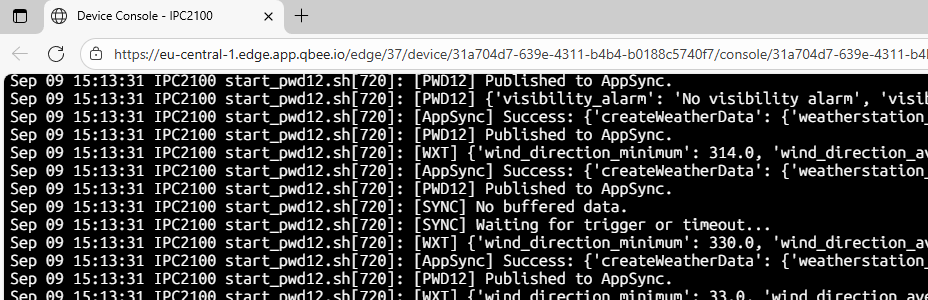
\includegraphics[width=0.9\textwidth]{images/qbee_logs.png}
  \caption{Example of live PWD12 sensor logs captured remotely through Qbee,
           showing parsed data, AppSync responses, and separate buffering events.}
  \label{fig:qbee-logs}
\end{figure}


\subsection{Cloud Data on AWS DynamoDB}

Once parsed and validated, sensor messages are uploaded to the cloud via AppSync and stored in an AWS DynamoDB table. Figure~\ref{fig:dynamodb-table} presents a snapshot of the table view, where each row corresponds to a single data record produced by the weather station. The key attributes visible in this view are the \texttt{created\_at} timestamp (in epoch format) and the \texttt{weatherstation\_id}, which uniquely identify when and where the measurement was taken. The \texttt{weather\_data} field, stored in JSON format, encapsulates the full set of parsed parameters such as visibility averages, present weather codes, precipitation intensity, and snow accumulation. This table therefore represents the chronological archive of all measurements transmitted by the PWD12 sensor, with each record aligned to the structure expected by downstream applications.

\begin{figure}[H]
  \centering
  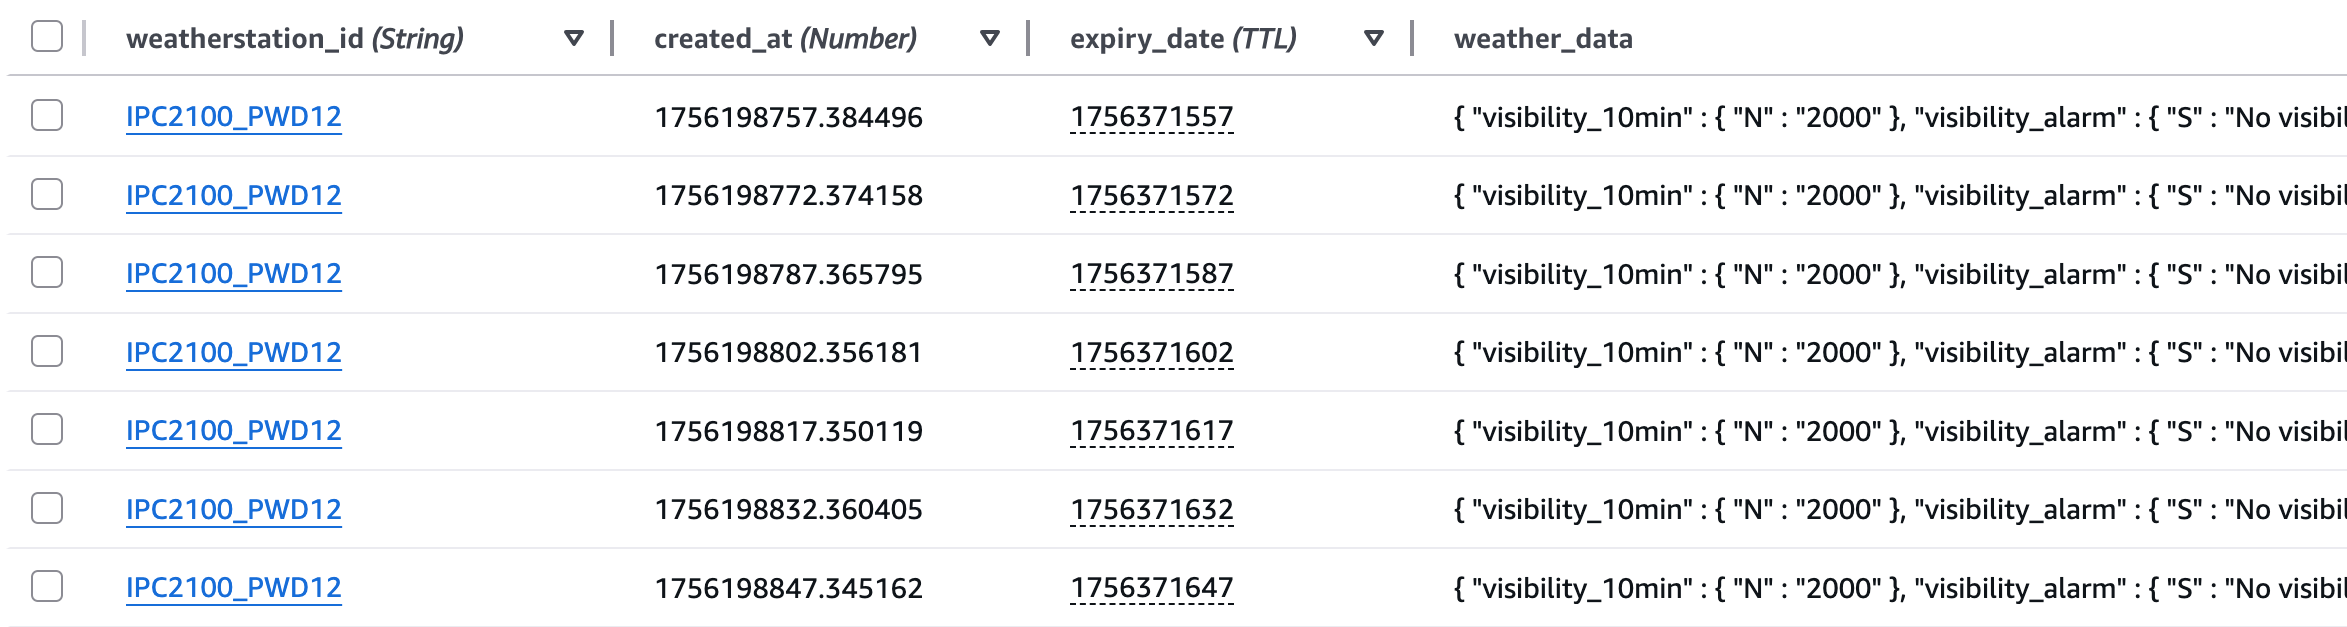
\includegraphics[width=\textwidth]{images/dynamodb_table.png}
  \caption{PWD12 sensor data stored in AWS DynamoDB. Each row corresponds to a structured measurement record with timestamp, station identifier, and JSON payload.}
  \label{fig:dynamodb-table}
\end{figure}

For clarity, Figure~\ref{fig:dynamodb-record} zooms into one specific record. This detailed view highlights how the parsed payload is stored in DynamoDB: the JSON string contains key-value pairs that mirror the structure defined in Section~\ref{sec:data_pipeline}. For example, the fields \texttt{visibility\_1min} and \texttt{visibility\_10min} provide rolling averages of measured visibility, while \texttt{present\_weather\_nws} and \texttt{present\_weather\_code\_inst} capture instantaneous and coded weather conditions. Precipitation values, such as \texttt{precip\_intensity} and \texttt{precip\_cumulative}, are also preserved. In addition, metadata such as the station identifier ensures that data from multiple deployed stations can be distinguished on the backend.

\begin{figure}[H]
  \centering
  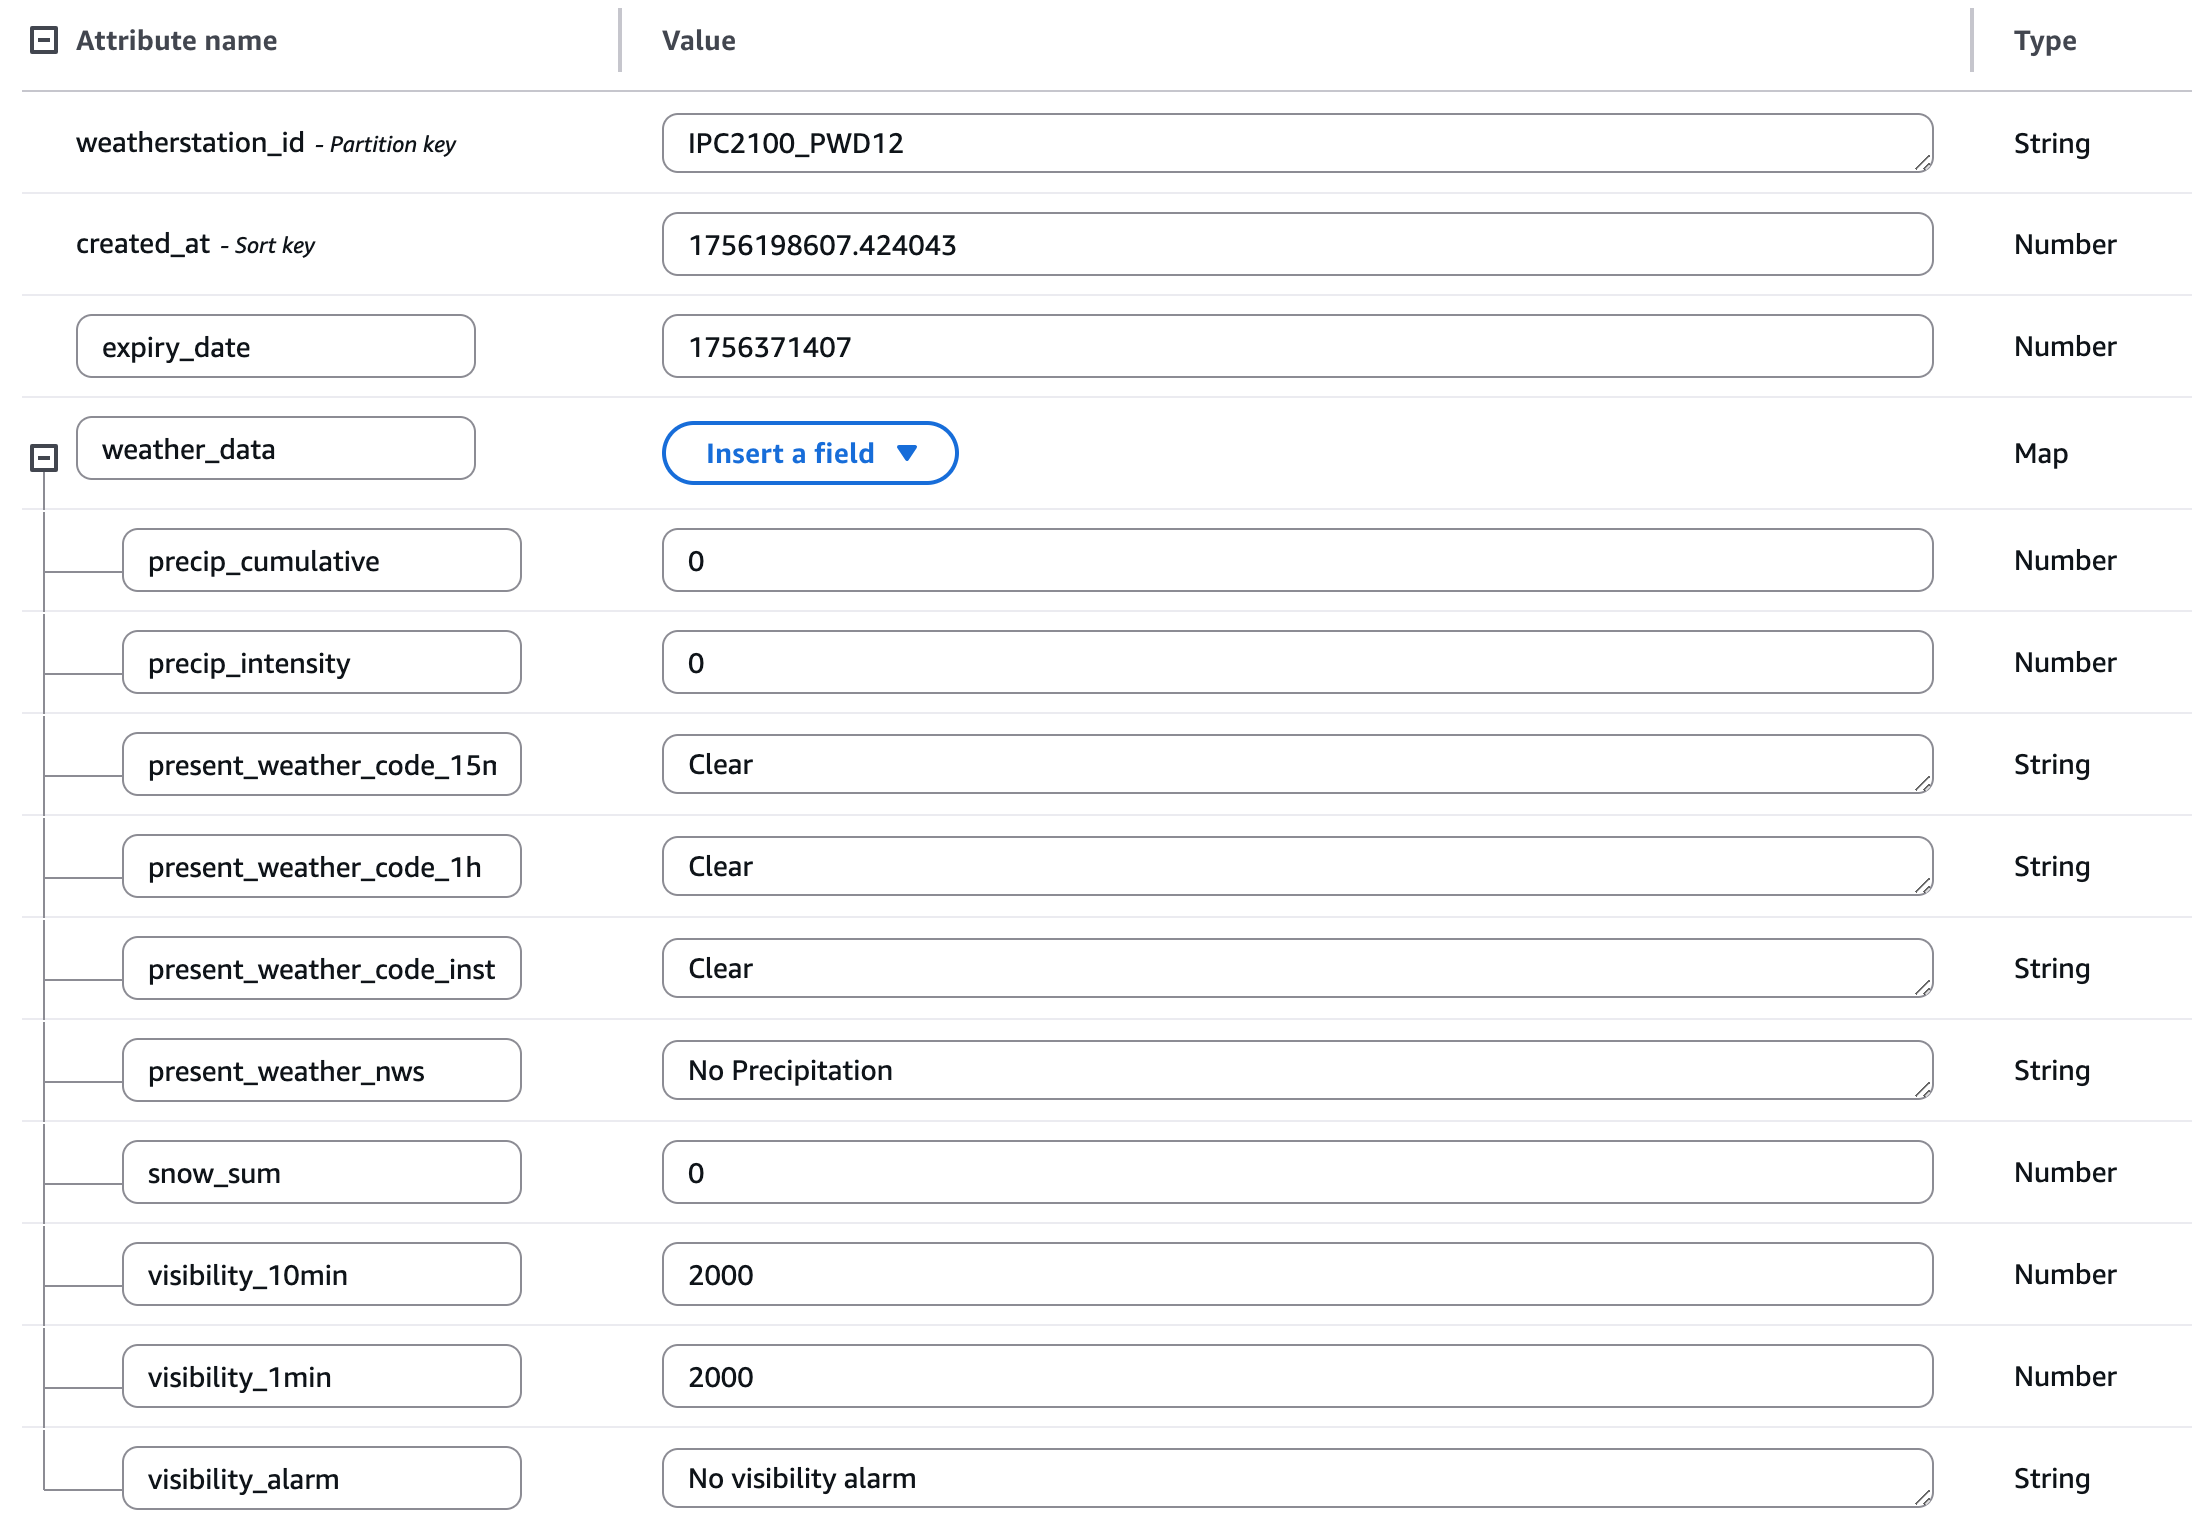
\includegraphics[width=0.85\textwidth]{images/dynamodb_record.png}
  \caption{Detailed view of a single PWD12 sensor record in DynamoDB.}
  \label{fig:dynamodb-record}
\end{figure}

Together, these two figures demonstrate the complete data persistence workflow: sensor messages generated by the PWD12 are parsed locally on the RevPi, buffered when connectivity is unavailable, and then ingested into DynamoDB in a structured format. The result is a reliable, queryable time series of weather data that can be consumed by higher-level services for monitoring, analytics, or flight planning. This confirms both the correctness of the parsing logic and the robustness of the cloud synchronization pipeline.

\subsection{Discussion of Results}

The screenshots illustrate that:
\begin{itemize}
    \item Sensor data is correctly read and parsed on the \gls{revpi}.
    \item Offline buffering and retry logic function as intended when connectivity is intermittent.
    \item Cloud synchronization to AWS AppSync and DynamoDB works reliably, with proper schema mapping and timestamp ordering.
\end{itemize}

These results confirm that the \gls{pwd12} integration provides operational visibility measurements in real-time, both locally and in the cloud, fulfilling the system design objectives.

\subsection{Field Validation and Bug Fixing}

To validate the integration in real-world conditions, the system was temporarily deployed on a rooftop installation in Konstanz. This short-term test allowed direct exposure of the sensors to outdoor weather, providing more realistic operating conditions compared to bench testing. 

During this deployment, several bugs were discovered, primarily related to parsing edge cases and intermittent communication errors. These were fixed iteratively, resulting in a more robust software pipeline capable of handling sensor noise and temporary data gaps. 

No pictures were recorded during this short-term rooftop test, but operational logs and observations confirmed the system’s functionality under real conditions. Representative log excerpts are shown in Figure~\ref{fig:field-validation}, highlighting successful message acquisition, parsing, and cloud transmission.

\begin{figure}[H]
  \centering
  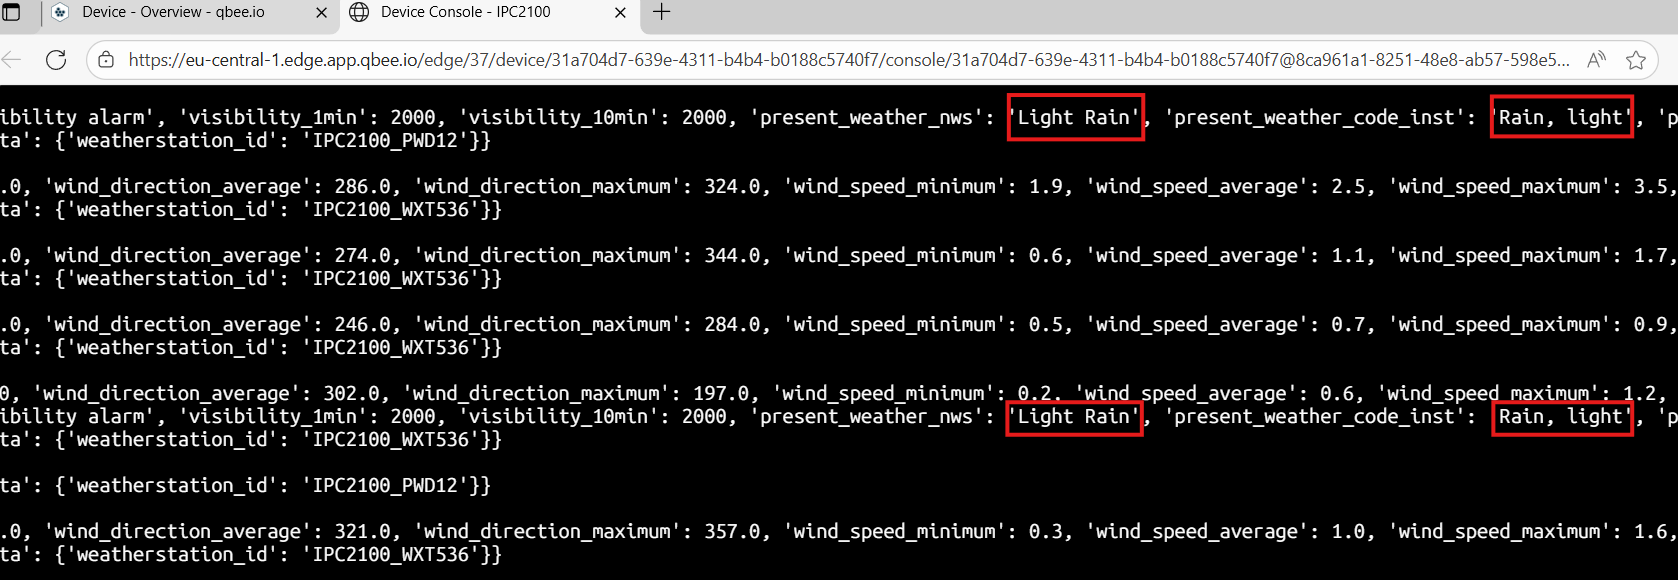
\includegraphics[width=\textwidth]{images/field_test_logs.png}
  \caption{Excerpts from live logs during the rooftop field test.}
  \label{fig:field-validation}
\end{figure}



\section*{Conclusion}

This chapter presented the complete integration of the Vaisala \gls{pwd12} sensor into the existing weather station system. Hardware adaptations enabled stable RS-485 communication, while modular Python components were developed for reading, parsing, and structuring sensor data. Robustness was ensured through local SQLite buffering with retry logic, and cloud synchronization was achieved via AppSync GraphQL mutations. Deployment under systemd provides long-term stability, security, and autonomous operation.





\cleardoublepage

\chapter*{General Conclusion}
\addcontentsline{toc}{chapter}{General Conclusion}

This thesis presented the design and implementation of an **IoT-based weather monitoring solution** that extends the capabilities of an existing weather station at Unisphere GmbH. 
The overall objective was to integrate visibility and present weather measurements while increasing the resilience of the system against temporary network disruptions.  

The work began with a study of the deployed infrastructure, which originally consisted of a single multisensor unit connected to a Revolution Pi industrial controller and synchronized with the cloud through AWS AppSync. 
While effective for parameters such as wind, temperature, humidity, and precipitation, this setup lacked both visibility monitoring and offline buffering, two features that are essential for reliable operation in the context of aviation and urban air mobility.  

To address these shortcomings, a new visibility sensor was examined in detail. 
Its measurement principle, installation constraints, and communication formats were analyzed, followed by bench tests that confirmed stable RS-485 operation at 9600~bps. 
A parsing logic was implemented to convert raw ASCII messages into structured JSON records aligned with the cloud schema. 
This ensured that data generated locally could be seamlessly integrated with Unisphere’s existing cloud services.  

Integration into the operational weather station required hardware and software adaptations. 
On the hardware side, the sensor was connected via a dedicated serial interface, with only power and RS-485 lines wired through an M12 connector. 
On the software side, modular Python components were developed to separate sensor reading, message parsing, and data serialization. 
These processes were executed under \texttt{systemd} to guarantee autonomous operation, automatic restart on failure, and secure long-term deployment.  

A critical contribution of this work was the addition of a local SQLite buffer. 
This mechanism stores data whenever connectivity is lost, retries synchronization once the network is restored, and guarantees the temporal order of measurements without duplication. 
Validation confirmed that several hundred entries could be buffered and recovered successfully, demonstrating a significant improvement in reliability compared to the previous version of the system.  

The complete workflow was validated through live Qbee logs and DynamoDB records, which confirmed successful acquisition, parsing, buffering, and synchronization of sensor data. 
Rooftop tests provided further evidence that the system functions correctly under real environmental conditions, with continuous acquisition and cloud delivery confirmed over several days of operation.  

Beyond these results, several perspectives open the way for future developments. 
At the cloud level, the GraphQL schema could be extended to support batch ingestion, improving efficiency for high-frequency deployments. 
A formal monitoring and alerting layer would strengthen operational reliability by enabling proactive maintenance. 
At the hardware level, additional sensors such as ceilometers could be integrated to enrich the range of meteorological parameters. 
Finally, scaling the solution across multiple stations would reinforce Unisphere’s U-Space weather services and provide reliable, localized data for flight planning and traffic management.  

In conclusion, this work delivered a resilient and extensible IoT weather monitoring system that enhances measurement coverage and ensures robust data availability. 
The results demonstrate the feasibility of integrating advanced sensors with industrial controllers, local buffering, and cloud synchronization in a modular framework. 
Such solutions are key enablers for safe and efficient operations in aviation and emerging urban air mobility environments.  

%\appendix

%\chapter{Code}


\phantomsection
\addcontentsline{toc}{chapter}{Bibliography}
\printbibliography

\cleardoublepage
\thispagestyle{empty}
\begin{center}
    \begin{tabular}{ m{2.5cm} m{10cm} m{2.5cm} }
        
\includegraphics[width=2.5cm]{images/insat.jpg} &
        \centering
        \begin{minipage}[c]{\linewidth}
            \centering
            {\small \textbf{REPUBLIC OF TUNISIA}}\\[0.15cm]
            {\small Ministry of Higher Education and Scientific Research}\\[0.15cm]
            {\small University of Carthage}\\[0.15cm]
            {\small National Institute of Applied Sciences and Technology}
        \end{minipage}
        &
        
\includegraphics[width=2.5cm]{images/unicar.png} \\
    \end{tabular}
\end{center}


\noindent\rule{\textwidth}{0.4pt}
\vspace{0.5cm}
% ------------------- English Abstract -------------------

{\textbf{Design and Implementation of a Comprehensive \acrshort{oee} Framework for an Automated Transport System}}\\[-0.5cm]
\noindent\rule{\textwidth}{0.4pt}
{\textbf{Abstract}}


\small
This graduation project presents an Overall Equipment Effectiveness (\acrshort{oee}) framework adapted to autonomous yard-logistics operations. The approach redefines Availability, Performance, and Quality for variable transport missions and integrates Operational Design Domain (\acrshort{odd}) constraints. A canonical data model and ingestion pipeline were developed to harmonise telemetry, manual logs, and weather data. The framework was implemented at transfer level and extended with mission-phase diagnostics. Industrial data demonstrated the calculation chain, while controlled synthetic scenarios validated the consistency and sensitivity of the implemented metrics.

\textbf{Keywords:} \acrshort{oee}, autonomous vehicle, yard logistics, \acrshort{odd}, canonical data model, mission-phase diagnostics


\vspace{0.5cm}

% ------------------- French Abstract -------------------


{\textbf{Conception et implémentation d’un cadre complet de TRS pour un système de transport automatisé}}\\ [-1cm]

\noindent\rule{\textwidth}{0.4pt}

{\textbf{Résumé}}


\begin{french}
\small
Ce projet présente un cadre de Taux de Rendement Synthétique (TRS) adapté aux opérations de transport autonome en environnement logistique. L’approche adapte la Disponibilité, la Performance et la Qualité aux missions variables et intègre les contraintes \acrshort{odd}. Un modèle de données canonique et une chaîne d’intégration ont été développés pour harmoniser les données télémétriques, les journaux manuels et les données météorologiques. Le cadre est appliqué au niveau des transferts et complété par une analyse des phases de mission.

\textbf{Mots-clés :} TRS, véhicule autonome, logistique de parc, \acrshort{odd}, modèle de données canonique, phases de mission
\end{french}


\vspace{0.5cm}

% ------------------- Arabic Abstract (native XeTeX RTL) -------------------
\artext{{\Large\bfseries تصميم وتنفيذ إطار شامل للفعالية الإجمالية للمعدات لنظام نقل آلي}}
\vspace{-0.3cm}
\noindent\rule{\textwidth}{0.4pt}

\artext{{\bfseries ملخص}}

\small
\artext{يقدّم هذا المشروع إطارًا للفعالية الإجمالية للمعدات (\acrshort{oee}) مكيّفًا مع عمليات النقل الذاتي في الساحات اللوجستية. يعتمد الإطار على تكييف مفاهيم الإتاحة والأداء والجودة مع طبيعة مهام النقل المتغيّرة، مع دمج قيود مجال التشغيل التصميمي (\acrshort{odd}). كما تم تطوير نموذج بيانات موحّد ومسار لمعالجة ودمج بيانات القياس الآلي والسجلات اليدوية والبيانات الجوية. طُبّق الإطار على مستوى عمليات النقل، مع إضافة طبقة تشخيصية على مستوى مراحل المهمة لتحديد مواقع الخسائر بشكل أدق. واستُخدمت البيانات الصناعية لإظهار سلسلة الحساب، بينما استُخدمت سيناريوهات اصطناعية مضبوطة للتحقق من اتساق المؤشرات وحساسيتها.}

\artext{{\bfseries الكلمات المفتاحية:} الفعالية الإجمالية للمعدات، المركبات الذاتية، لوجستيات الساحات، \acrshort{odd}، نموذج البيانات، مراقبة الأداء، مراحل المهمة}



\end{document}
